\documentclass[t,aspectratio=169]{beamer}
\usepackage[T2A]{fontenc}
\usepackage[utf8]{inputenc}
\usepackage[russian,english]{babel}
\usepackage{graphicx}
\usepackage{commath}
\usepackage{tikz}
\usepackage{tikz-feynman}
\usepackage{tikz-3dplot}
\usetikzlibrary{arrows,automata,backgrounds,calendar,chains,matrix,mindmap,
    patterns,petri,shadows,shapes.geometric,shapes.misc,spy,trees,calc}
\usepackage{verbatim}
\usepackage{listings}

%%% Some definitions for math
\usepackage{amsmath}
\usepackage{bbm}

\setbeamertemplate{navigation symbols}{}
\setbeamertemplate{footline}[frame number]

\usepackage{comment}
\usepackage{url}
\usepackage{mathtools}
\usefonttheme[onlymath]{serif}
\graphicspath{{./images/}}
\title{Физика}
\subtitle {Введение}
\institute[TUM E18]{Technical University of Munich\\
Department of Physics, E18}
\author[Андрей Рабусов~\url{a.rabusov@tum.de}]{\texorpdfstring{Андрей Рабусов \newline\url{a.rabusov@tum.de}}{Андрей Рабусов}}

\date{13 Апреля 2022}


\newcommand{\backupbegin}{
\newcounter{finalframe}
\setcounter{finalframe}{\value{framenumber}}
}
\newcommand{\backupend}{
\setcounter{framenumber}{\value{finalframe}}
}
\begin{document}
\pdfinfo{
/Author (Andrei Rabusov)
/Title  (physics)
/Subject (intro)
}

\begin{frame}
\maketitle
\end{frame}
\begin{frame}{Содержание}
\tableofcontents[sectionstyle=show,subsectionstyle=show]
\end{frame}
\section{Введение}
\begin{frame}
    \frametitle{Сферы высказываний}
    \begin{columns}
        \begin{column}{0.5\textwidth}
            В аксиоматике социологии выделяют различные автономные сферы
            человеческого действия по принципам:
            \begin{itemize}[<+->]
                \item Свой язык
                \item Своя логика
                \item Своя рациональность
                \item Свой способ производства высказываний и действий
            \end{itemize}
        \end{column}
        \begin{column}{0.5\textwidth}
            Замкнутые системы согласно этой аксиоматике:
            \begin{itemize}[<+->]
                \item Философия
                \item Религия
                \item Искусство
                \item Политика
                \item Наука
            \end{itemize}
        \end{column}
    \end{columns}
\end{frame}

\begin{frame}
    \frametitle{Замкнутые системы}
    \only<1->{
        Философия: познание наиболее базовых принципов изучения мира, человека,
        и отношений между людьми
    }
    \only<2->{
        \par\vspace{0.3cm}
        Религия (обычно): отношение к непознаваемому
    }
    \par\vspace{0.3cm}
    \only<3->{
        Искусство: образное осмысление действительности
    }
    \only<4->{
        \par\vspace{0.3cm}
        Политика: совершение активных действий для изменения или консервации
        текущего положения дел
    }
    \only<5->{
        \par\vspace{0.3cm}
        Наука: познание мира
    }
\end{frame}


\begin{frame}
    \frametitle{Наука}
    \only<1->{
        \par\vspace{0.3cm}
        Математика: наука об отношениях между формальными объектами
    }
    \only<2->{
        \par\vspace{0.3cm}
        Лингвистика: наука о языках
    }
    \only<3->{
        \par\vspace{0.3cm}
        Социология: наука об отношениях между группами людей
    }
    \only<4->{
        \par\vspace{0.3cm}
        Психология: наука о психической деятельности людей и
        групп людей
    }
    \only<5->{
        \par\vspace{0.3cm}
        Химия: наука о веществе на молекулярном уровне
    }
    \only<6->{
        \par\vspace{0.3cm}
        Биология: наука о живой материи
    }
    \only<7->{
        \par\vspace{0.3cm}
        Музыкознание: наука о музыке
    }
\end{frame}

\section{Физика элементарных частиц}
\begin{frame}{Table of section content}
    \tableofcontents[currentsection, subsectionstyle=show/show/hide]
\end{frame}
\subsection{Частицы}
\begin{frame}
    \begin{figure}
        \begin{centering}
            \includegraphics[width=0.7\textwidth]{sm}
        \end{centering}
    \end{figure}
\end{frame}

\subsection{Ускорители}
\begin{frame}
    \begin{columns}
        \begin{column}{0.5\textwidth}
            \begin{figure}
                \begin{centering}
                    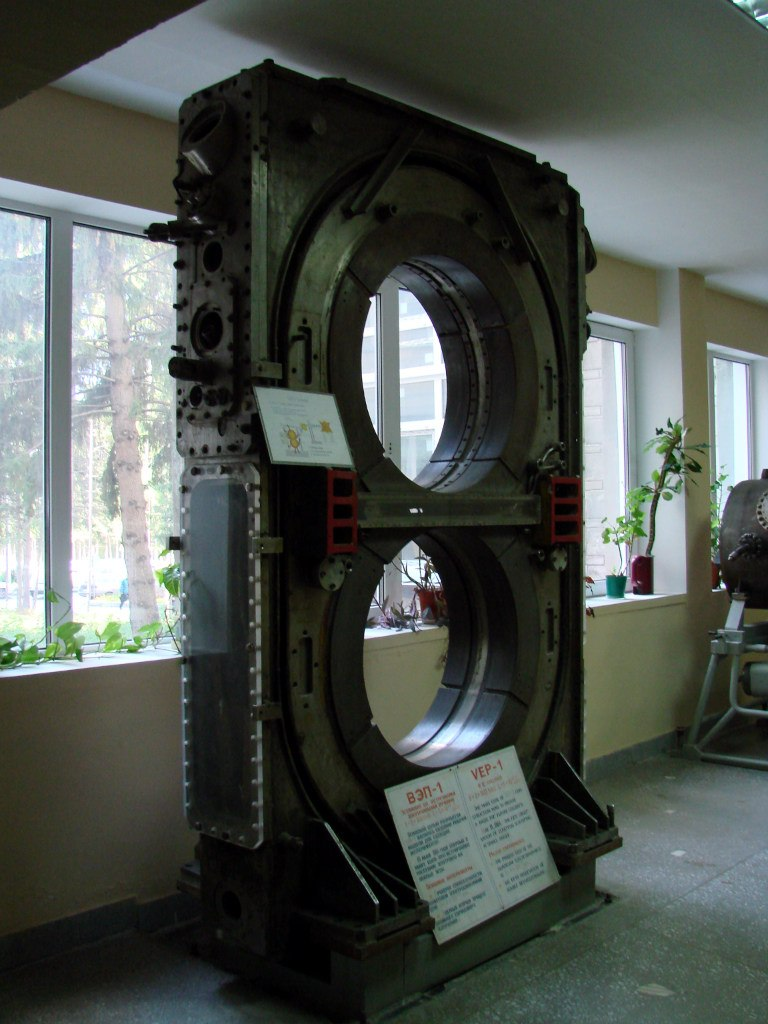
\includegraphics[width=0.7\textwidth]{vepp1}
                \end{centering}
            \end{figure}
        \end{column}
        \begin{column}{0.5\textwidth}
            \begin{figure}
                \begin{centering}
                    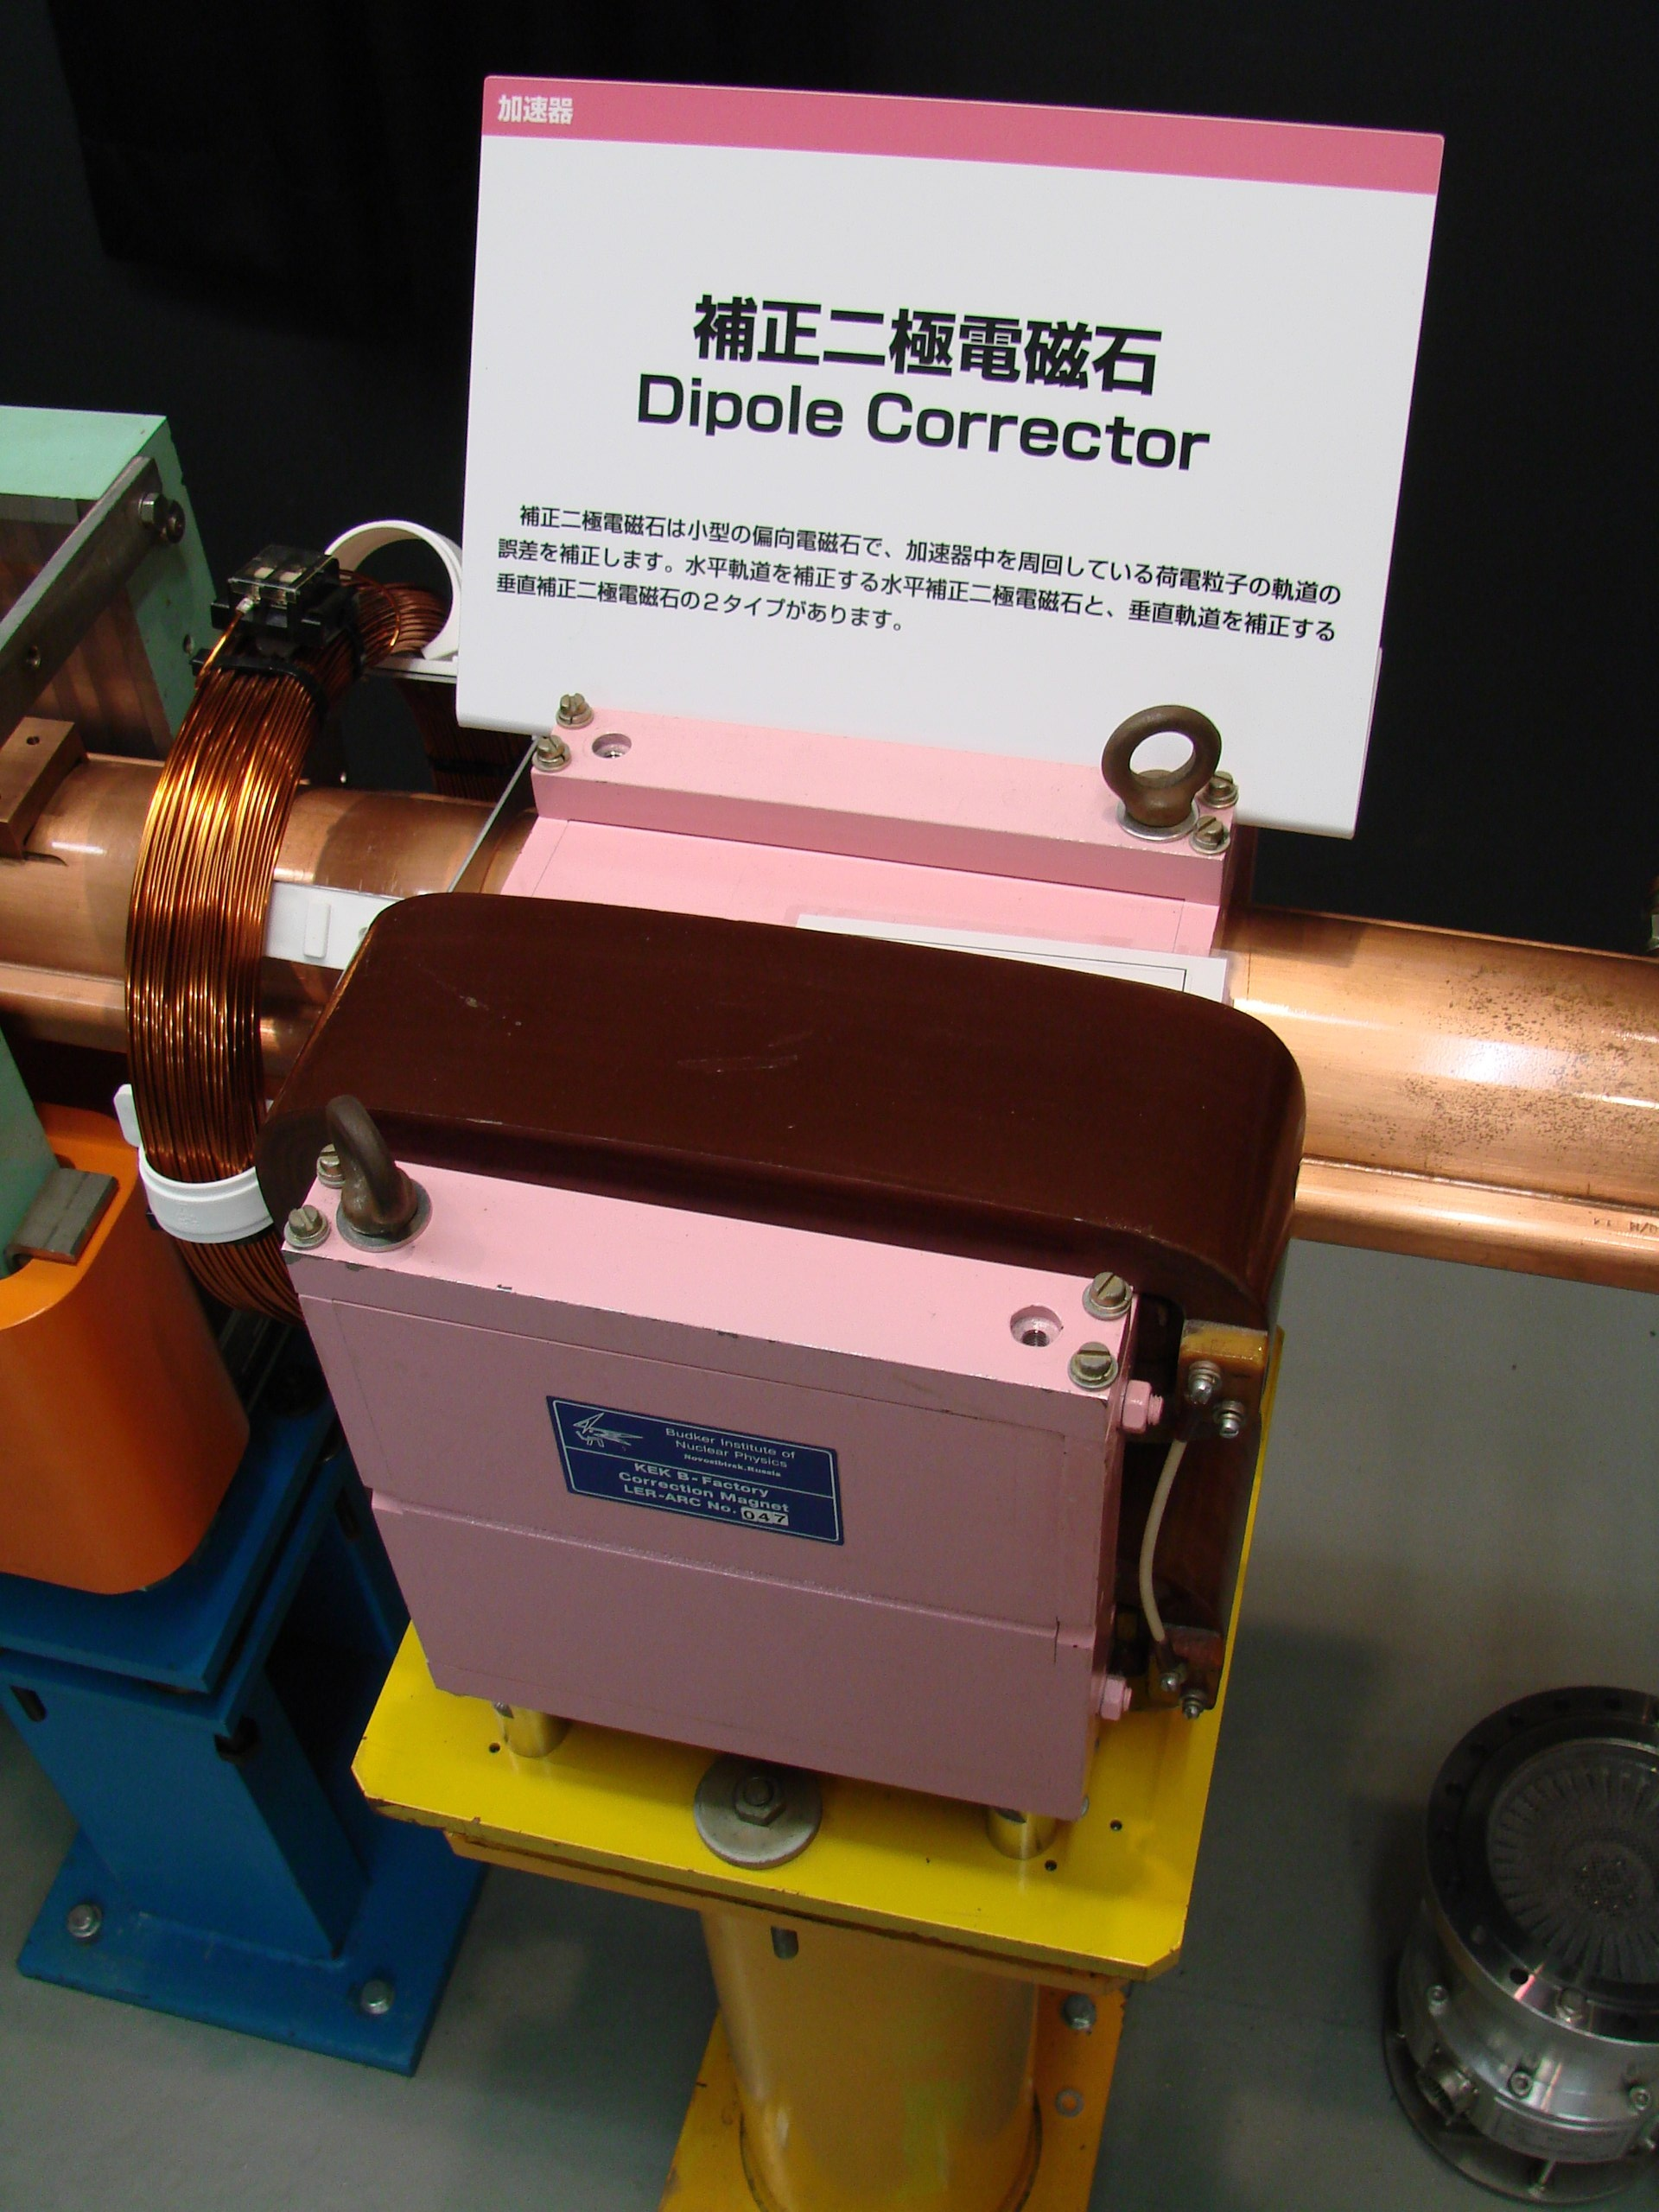
\includegraphics[width=0.7\textwidth]{dipole}
                \end{centering}
            \end{figure}
        \end{column}
    \end{columns}
\end{frame}


\begin{frame}
    \begin{figure}
        \begin{centering}
            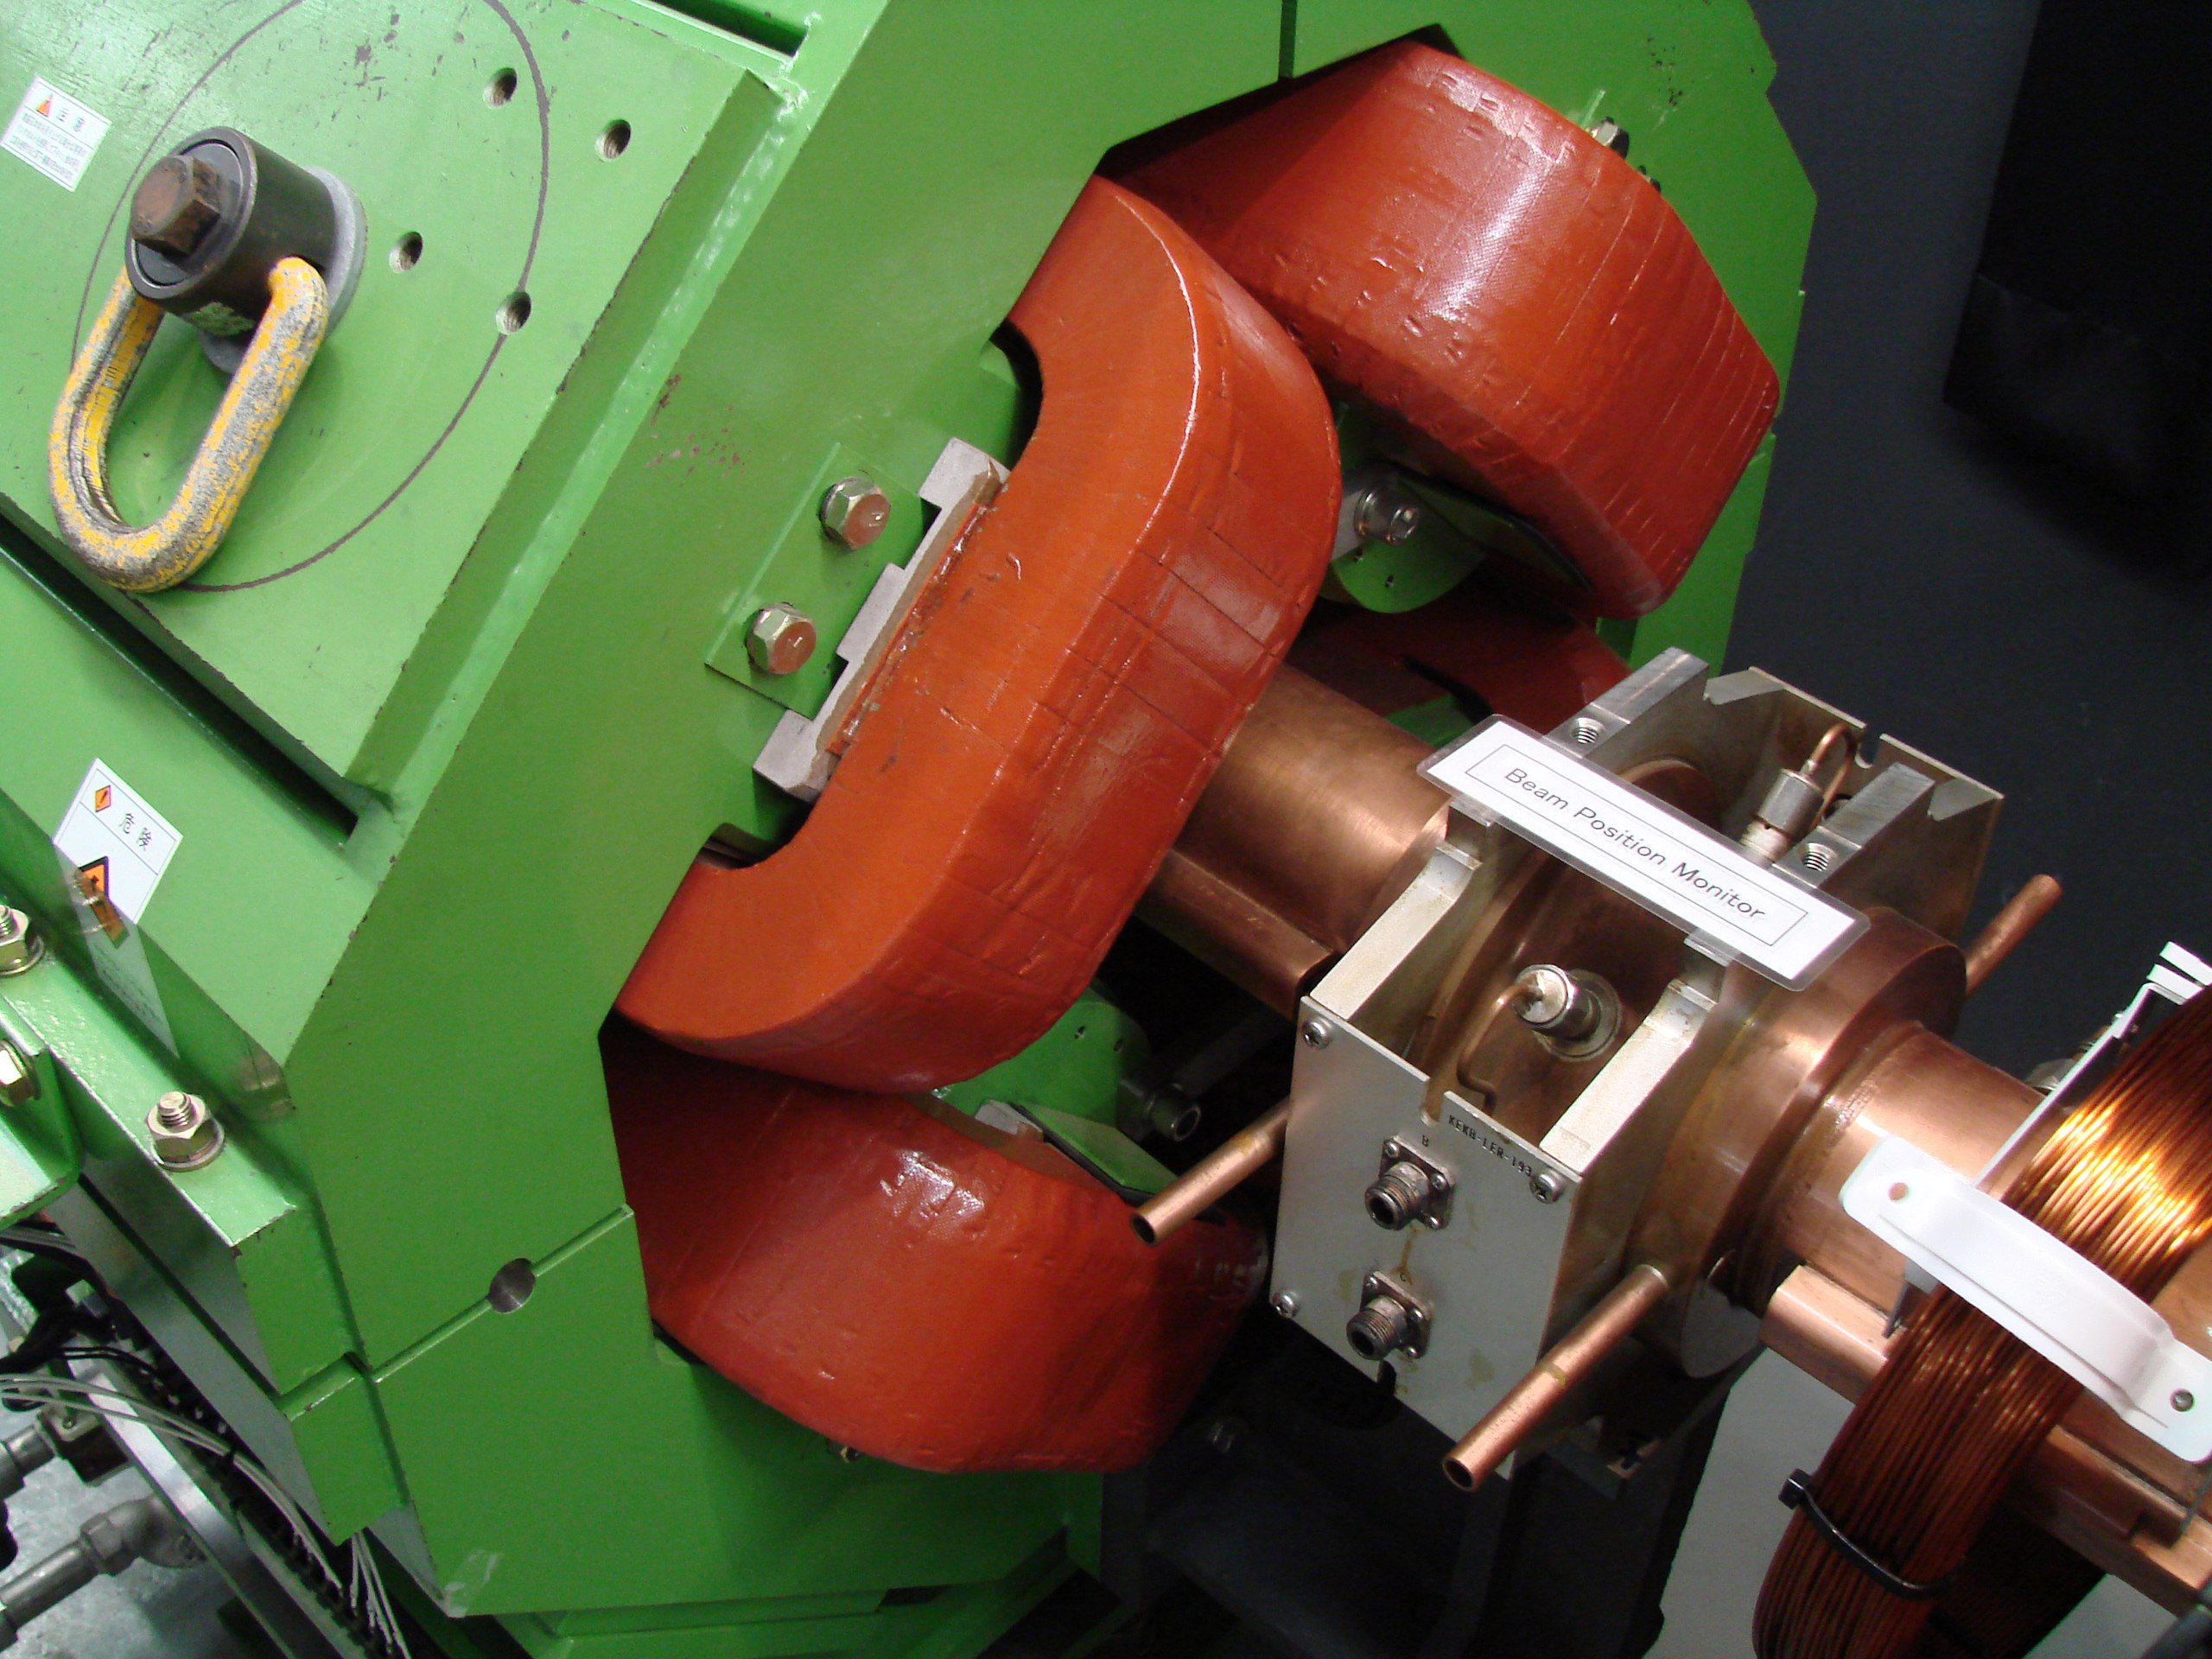
\includegraphics[width=0.7\textwidth]{quadrupole}
        \end{centering}
    \end{figure}
\end{frame}
\begin{frame}
    \begin{figure}
        \begin{centering}
            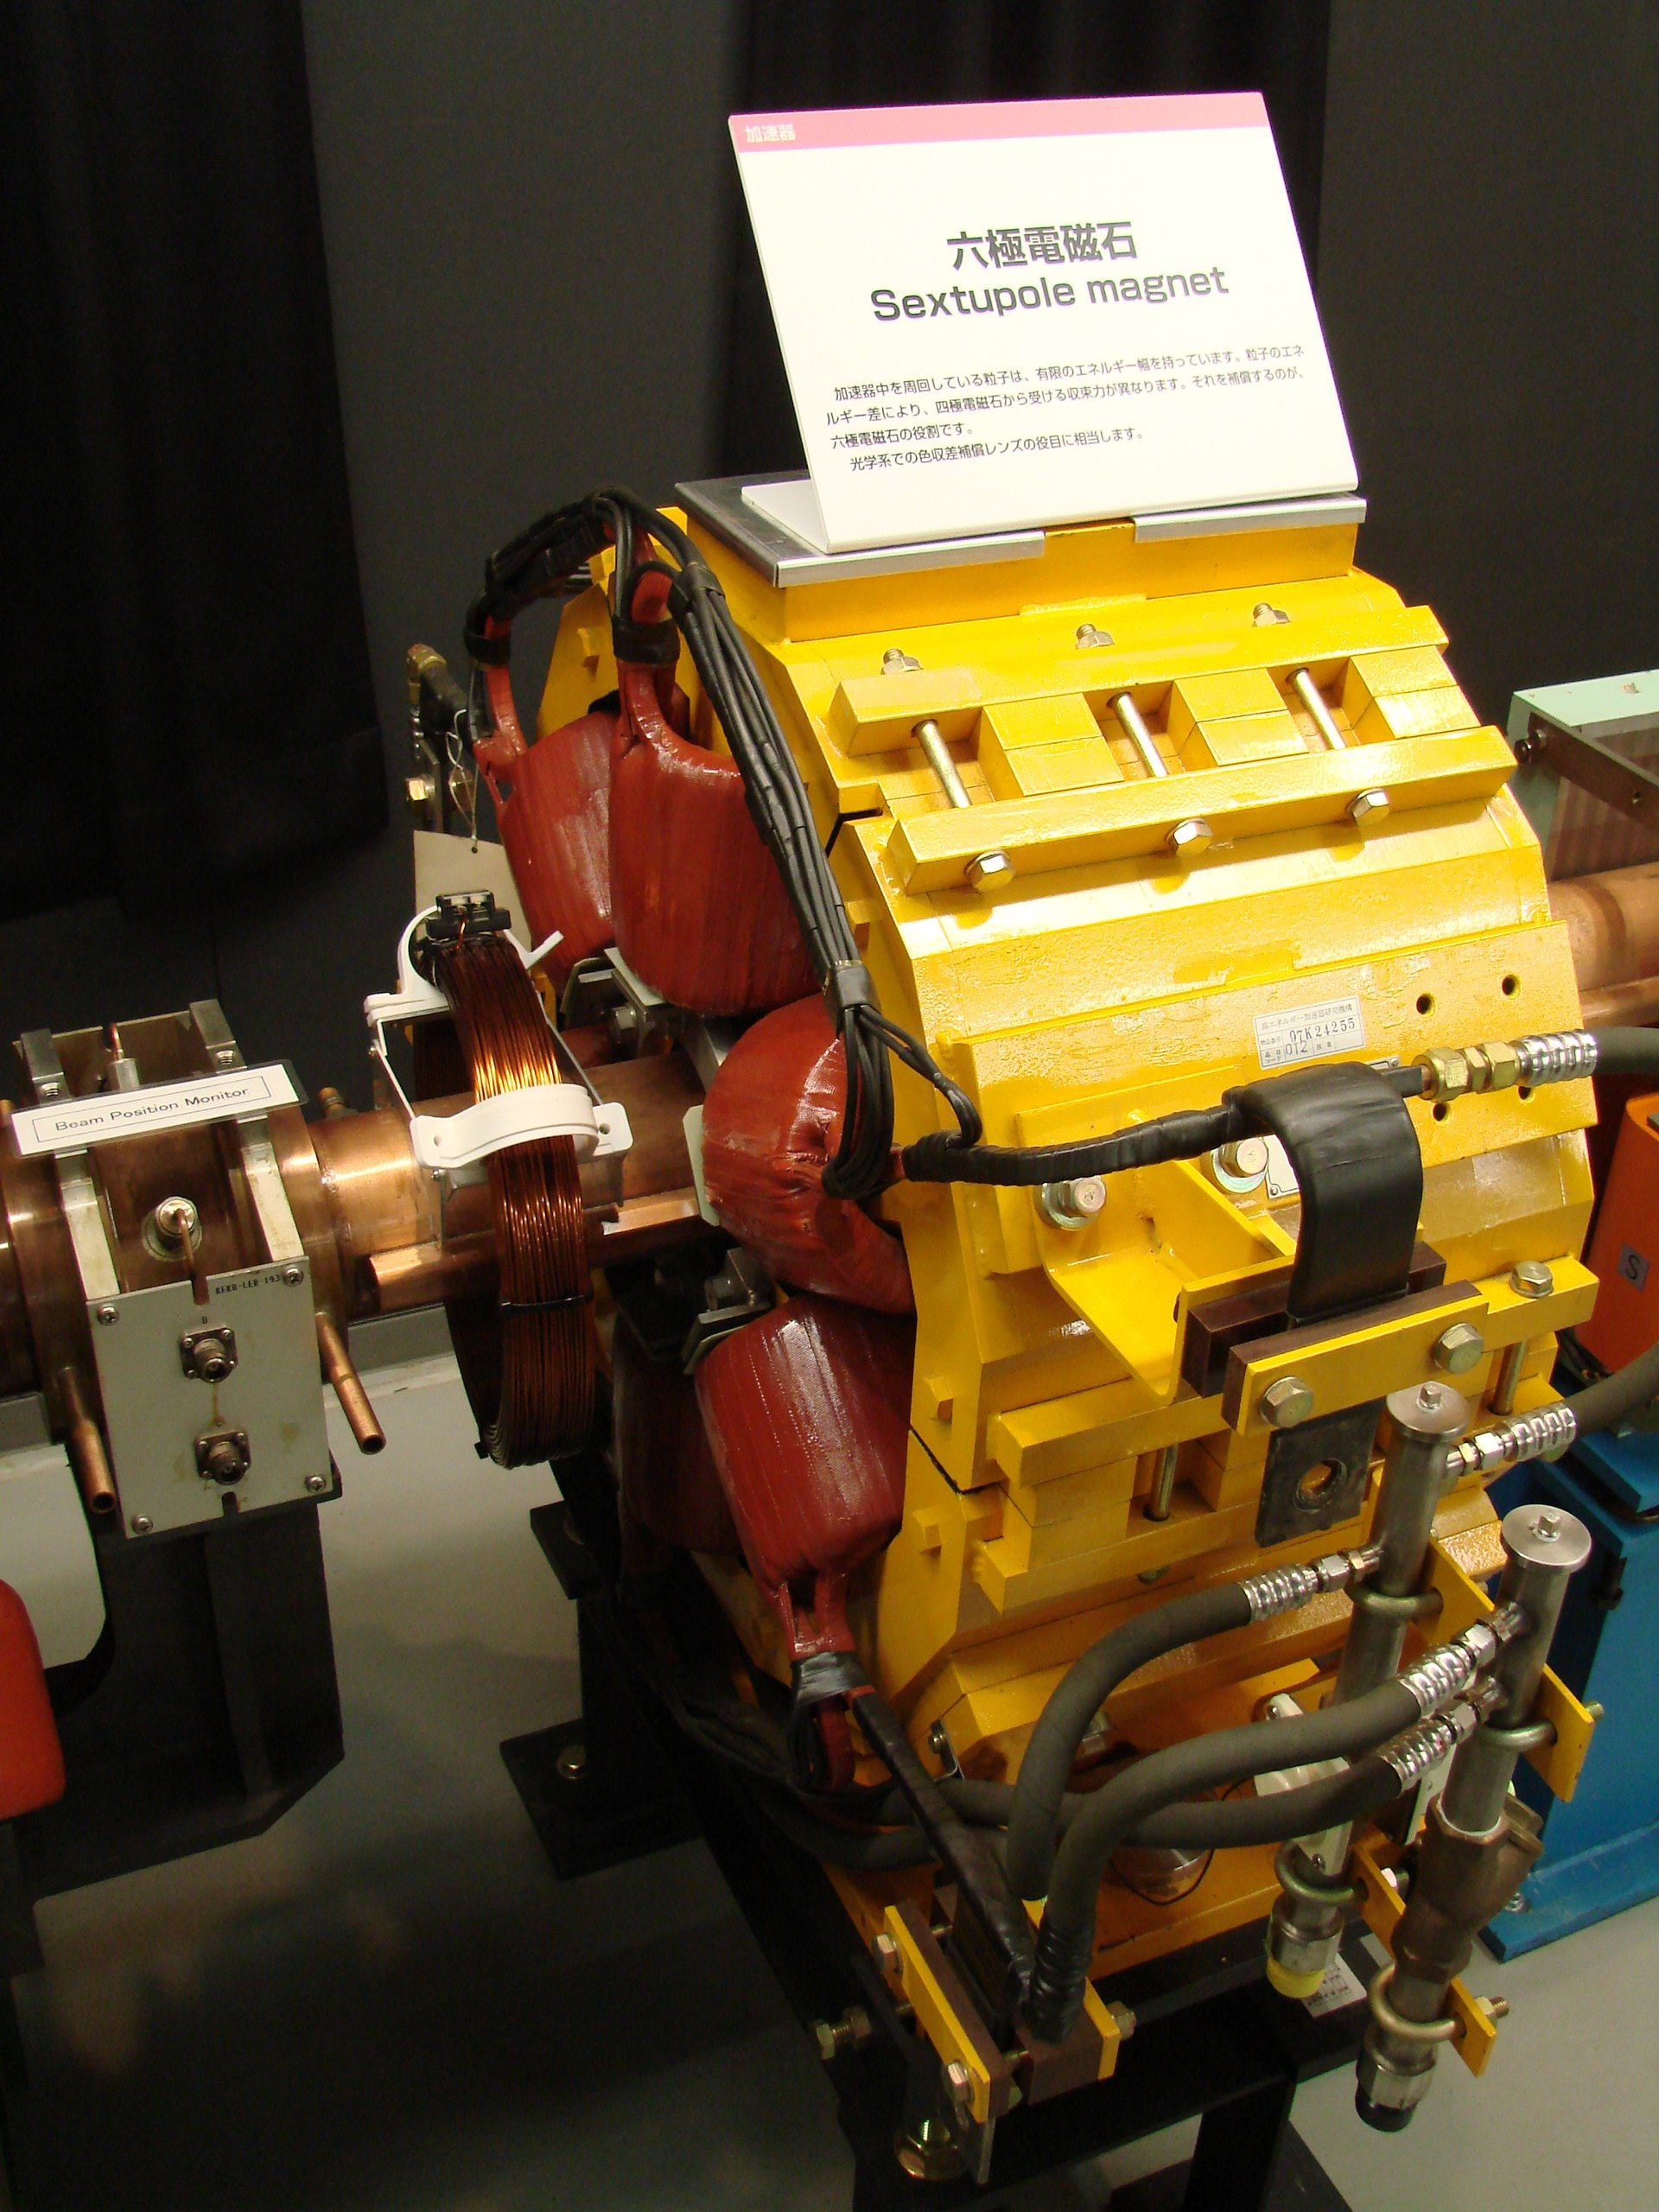
\includegraphics[width=0.7\textwidth]{sextupole}
        \end{centering}
    \end{figure}
\end{frame}

\begin{frame}
    \frametitle{Электрон-позитронный коллайдер}
    \begin{figure}
        \begin{centering}
            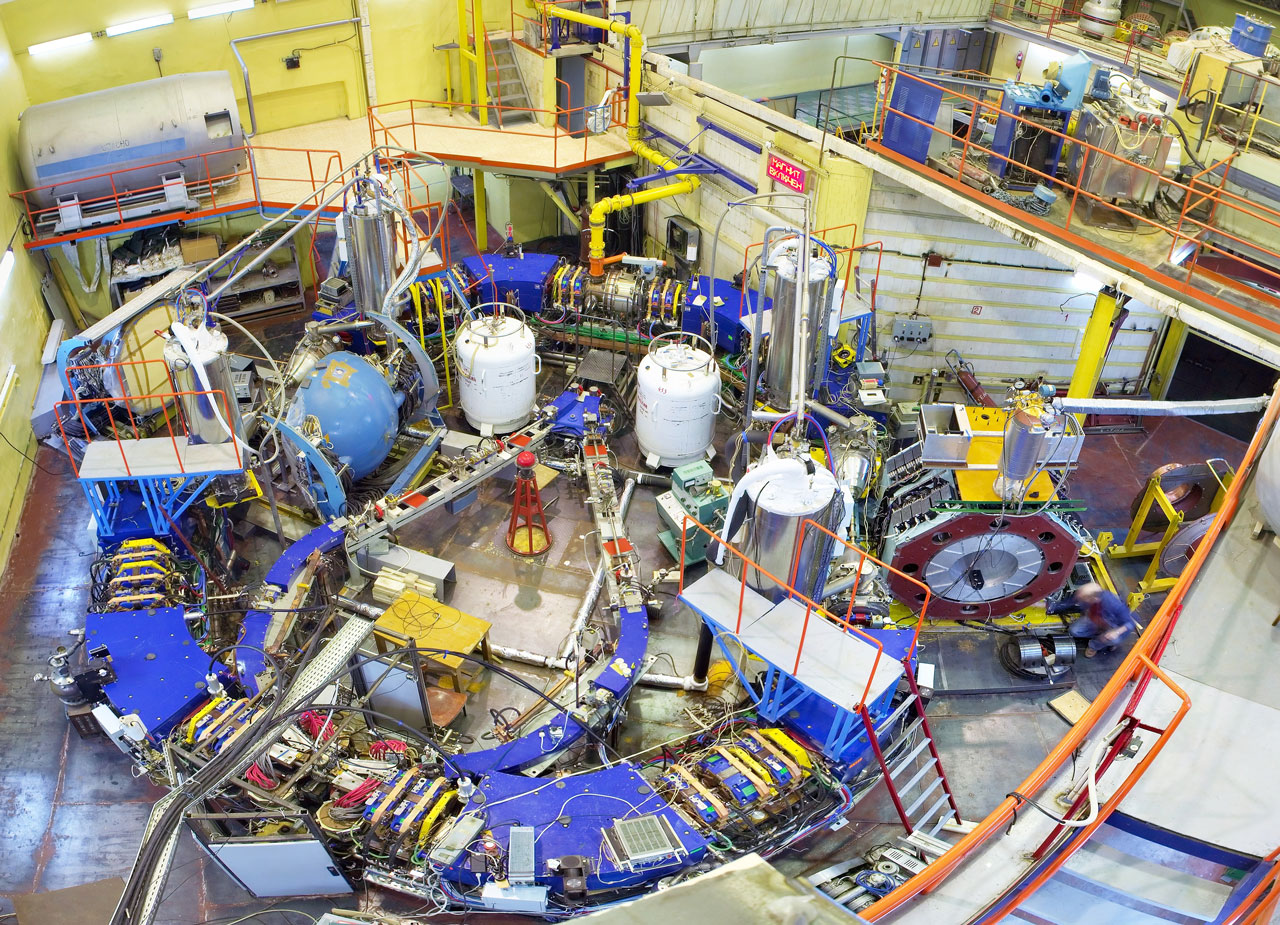
\includegraphics[width=0.7\textwidth]{vepp2}
        \end{centering}
    \end{figure}
\end{frame}

\subsection{Детекторы}
\begin{frame}
    \frametitle{Сферический детектор}
    \begin{figure}
        \begin{centering}
            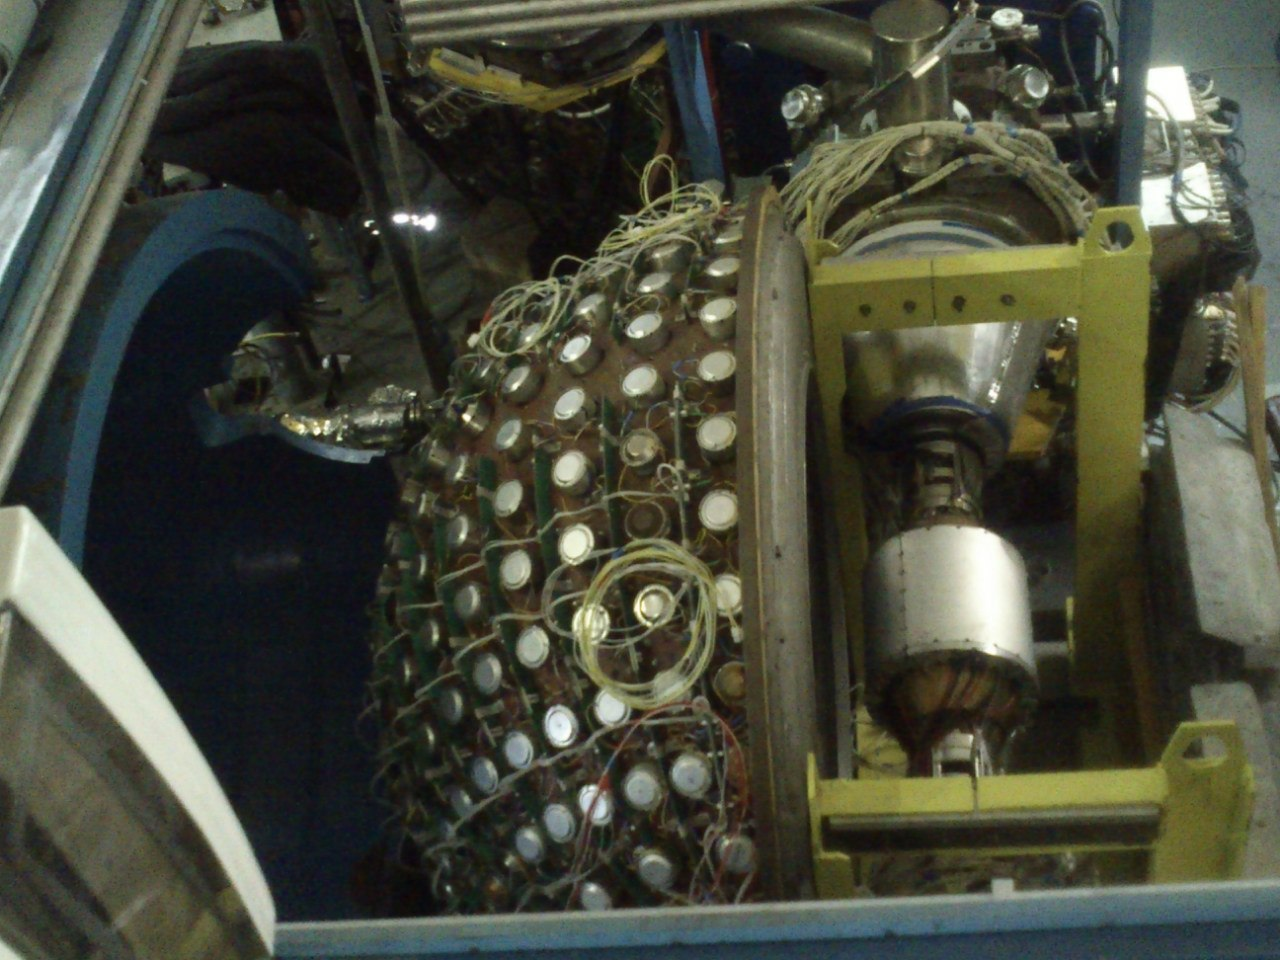
\includegraphics[width=0.7\textwidth]{snd}
        \end{centering}
    \end{figure}
\end{frame}
\begin{frame}
    \frametitle{Сферический детектор}
    \begin{figure}
        \begin{centering}
            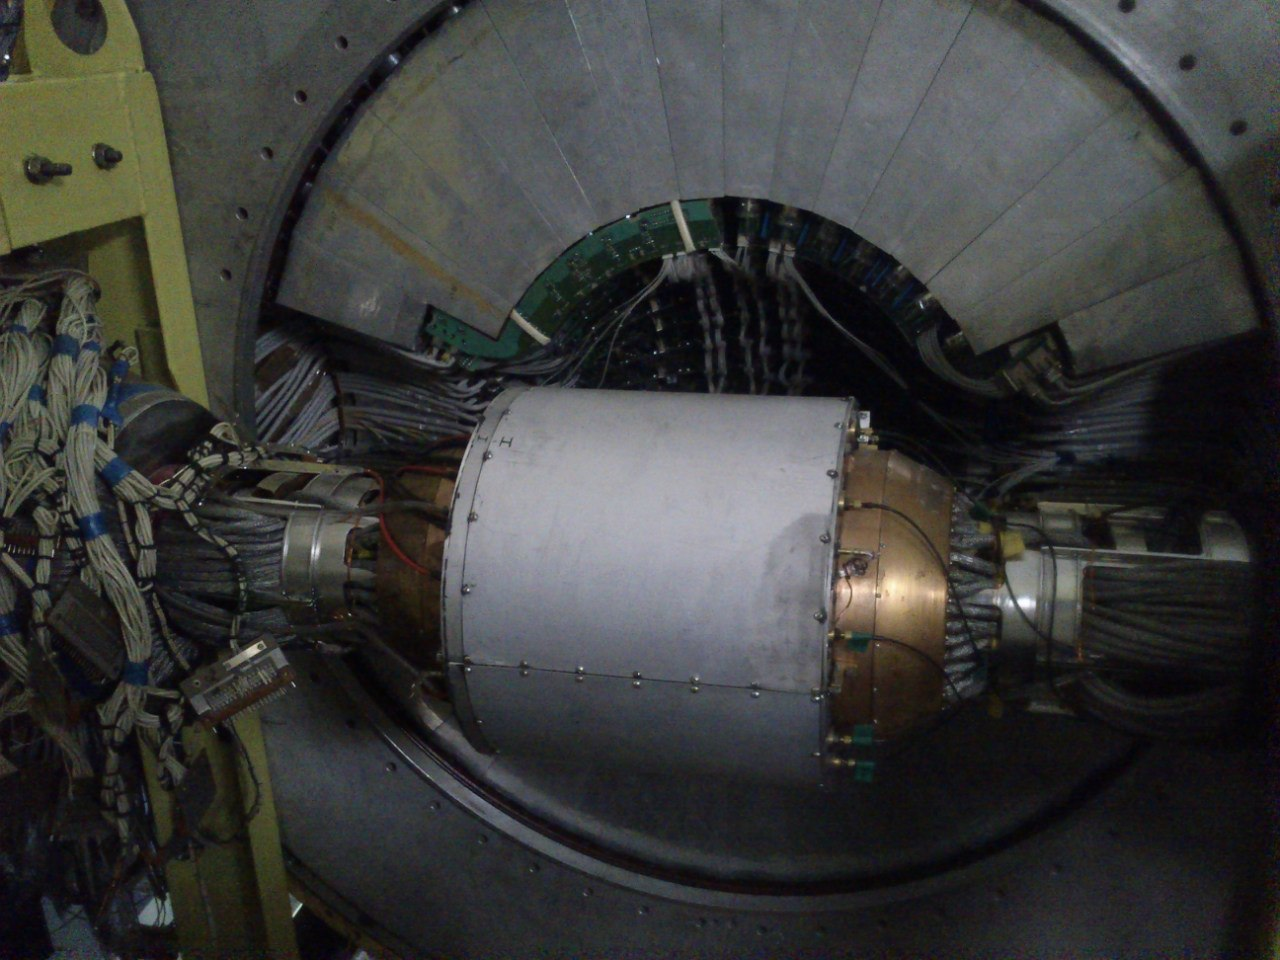
\includegraphics[width=0.7\textwidth]{snd-1st-half}
        \end{centering}
    \end{figure}
\end{frame}
\begin{frame}
    \frametitle{Сферический детектор}
    \begin{figure}
        \begin{centering}
            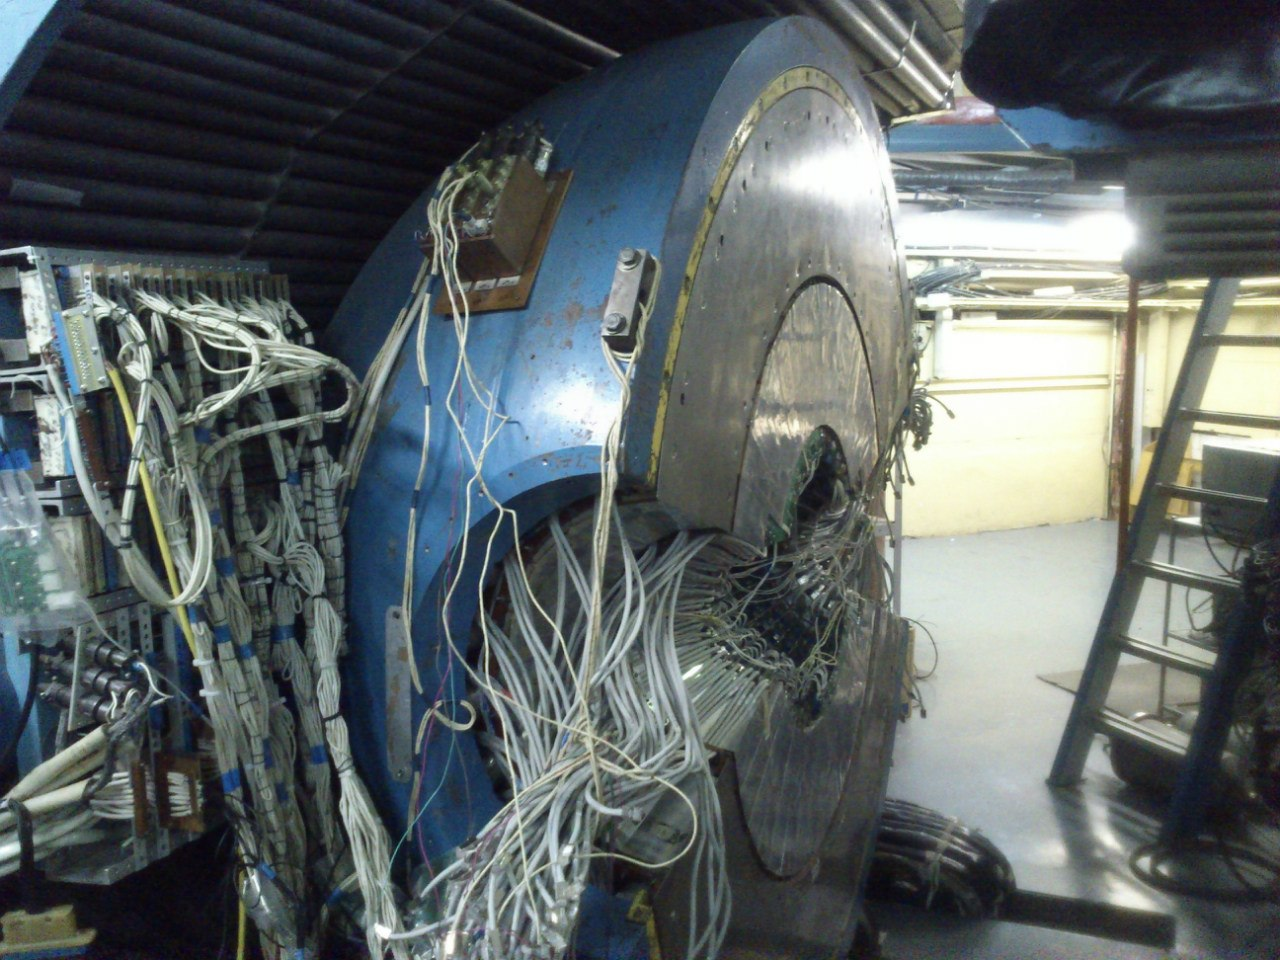
\includegraphics[width=0.7\textwidth]{snd-2nd-half}
        \end{centering}
    \end{figure}
\end{frame}

\subsection{B-фабрика}
\begin{frame}
    \begin{figure}
    {\LARGE Японская фабрика B-мезонов}
    \end{figure}
\end{frame}
\begin{frame}
    \frametitle{Точки выхода на поверхность}
    \begin{figure}
        \begin{centering}
            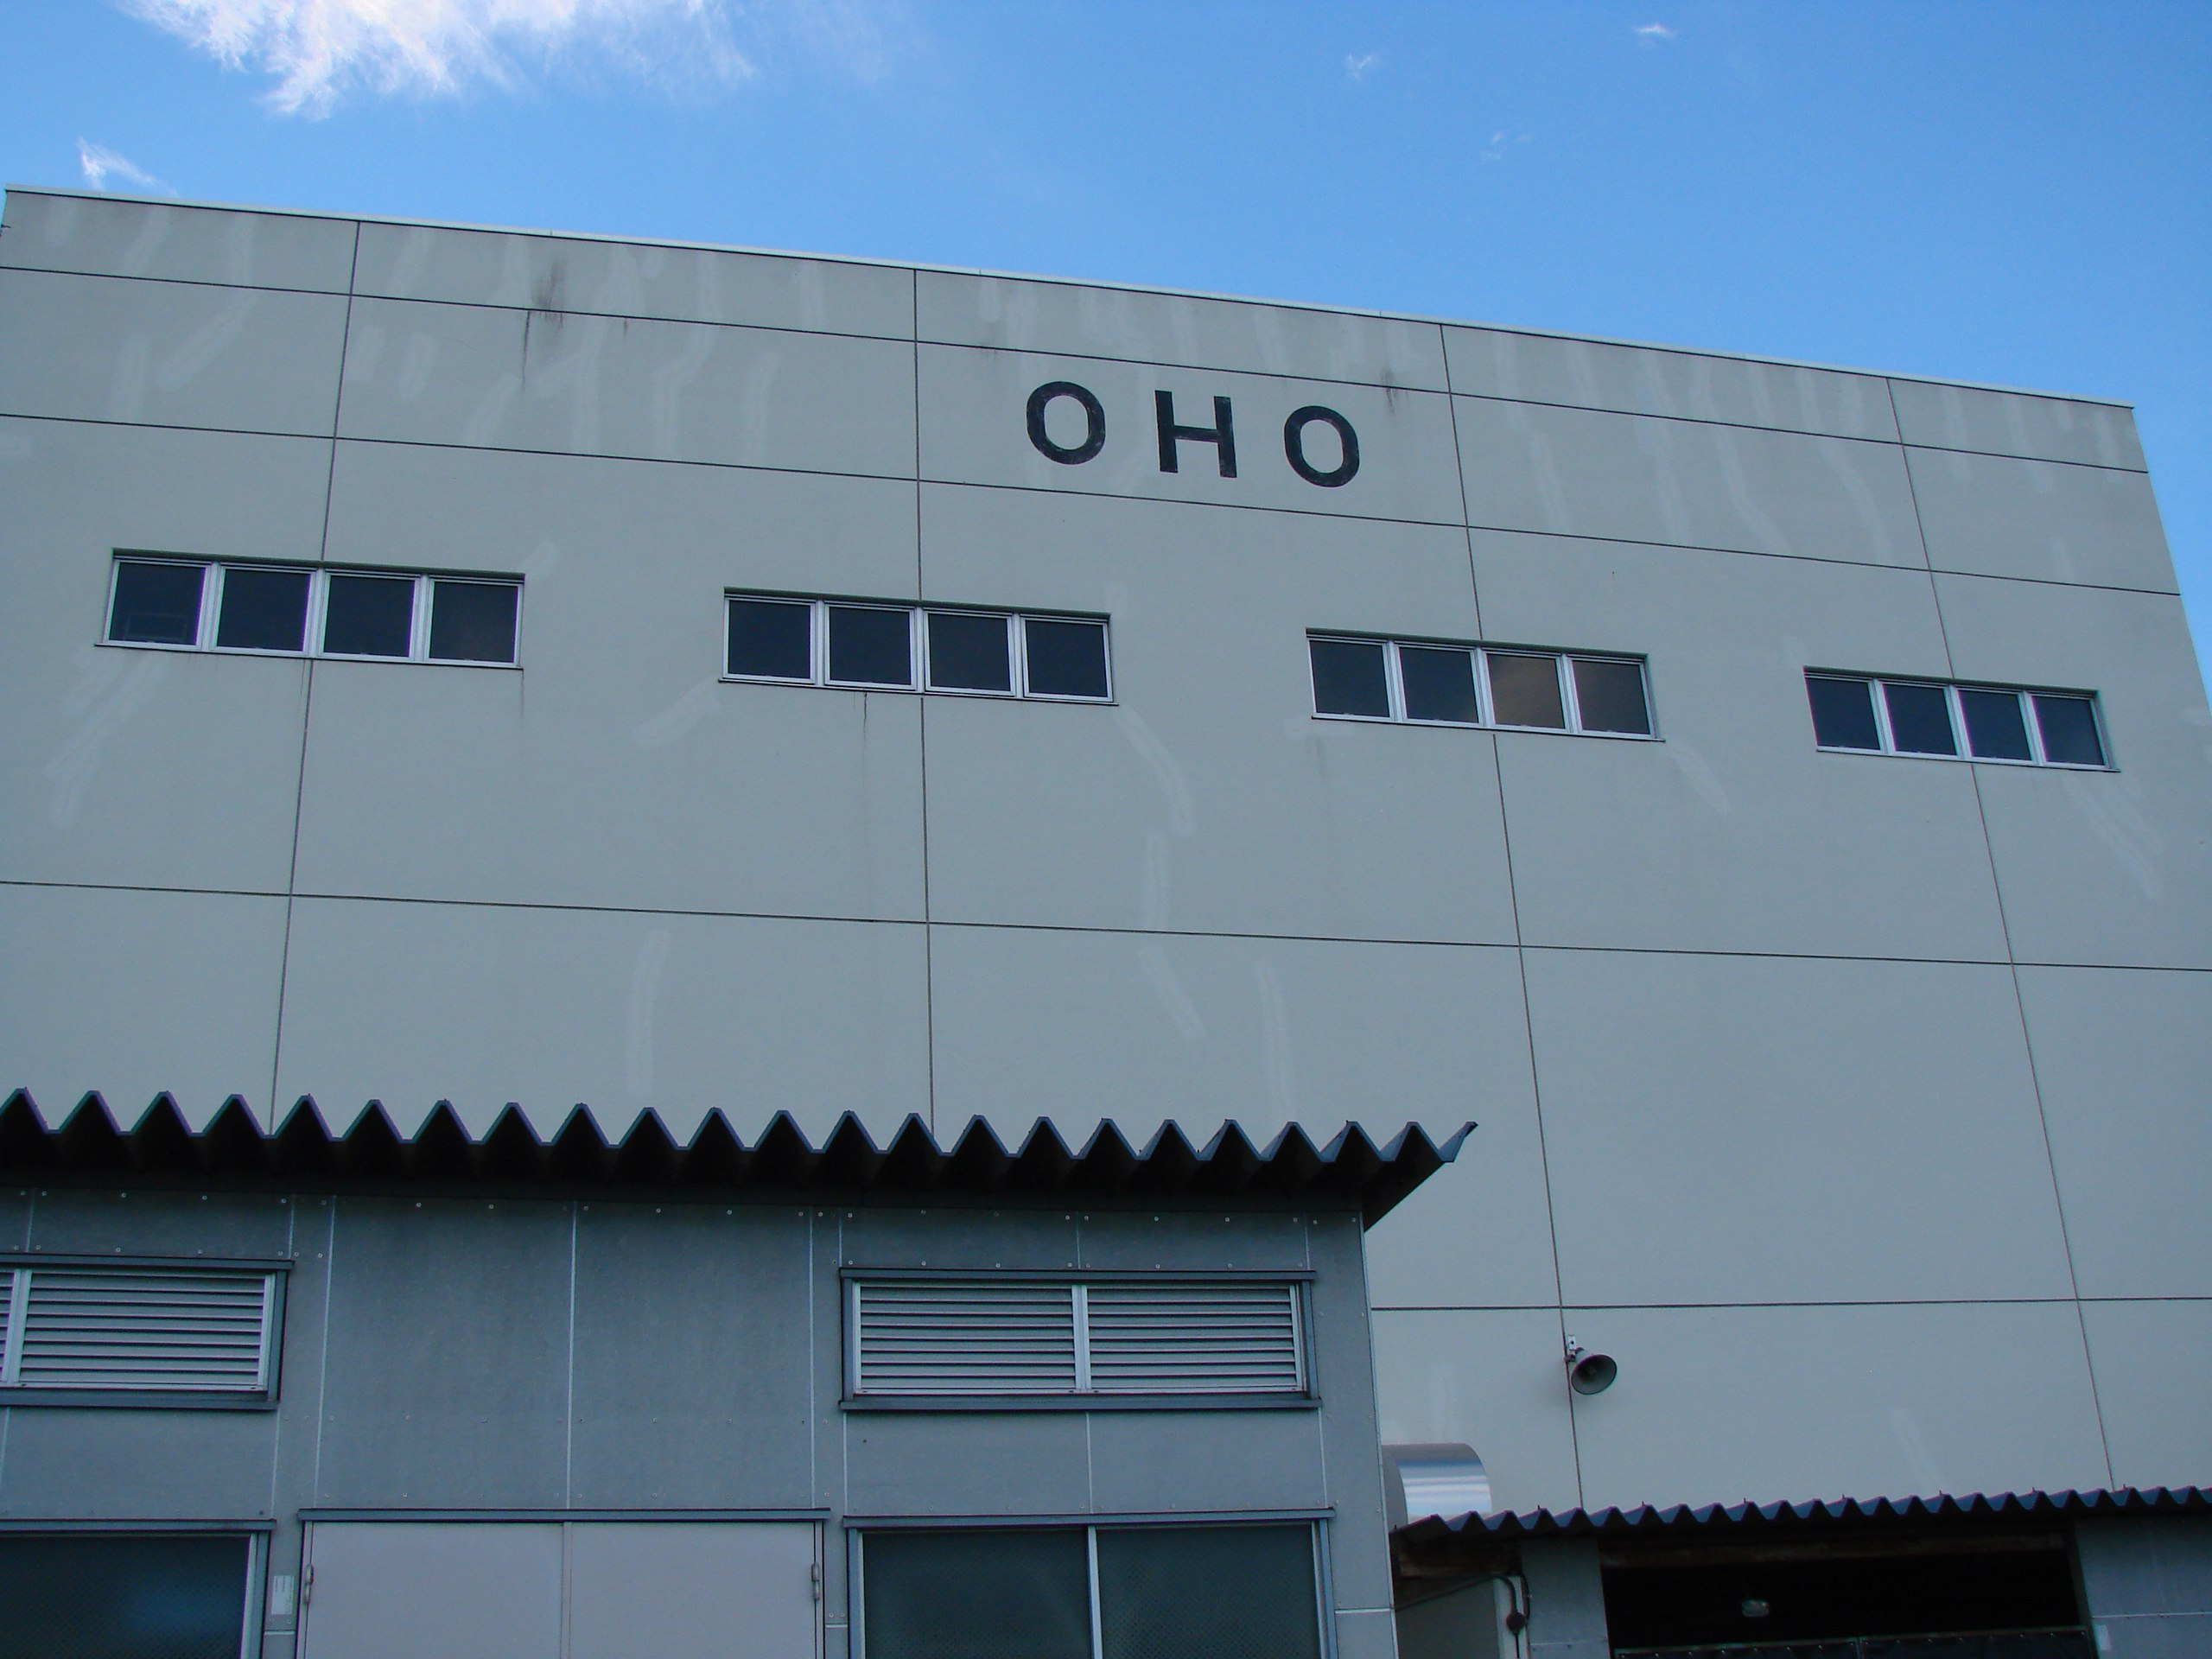
\includegraphics[width=0.7\textwidth]{oho}
        \end{centering}
    \end{figure}
\end{frame}
\begin{frame}
    \frametitle{Точки выхода на поверхность: детектор}
    \begin{figure}
        \begin{centering}
            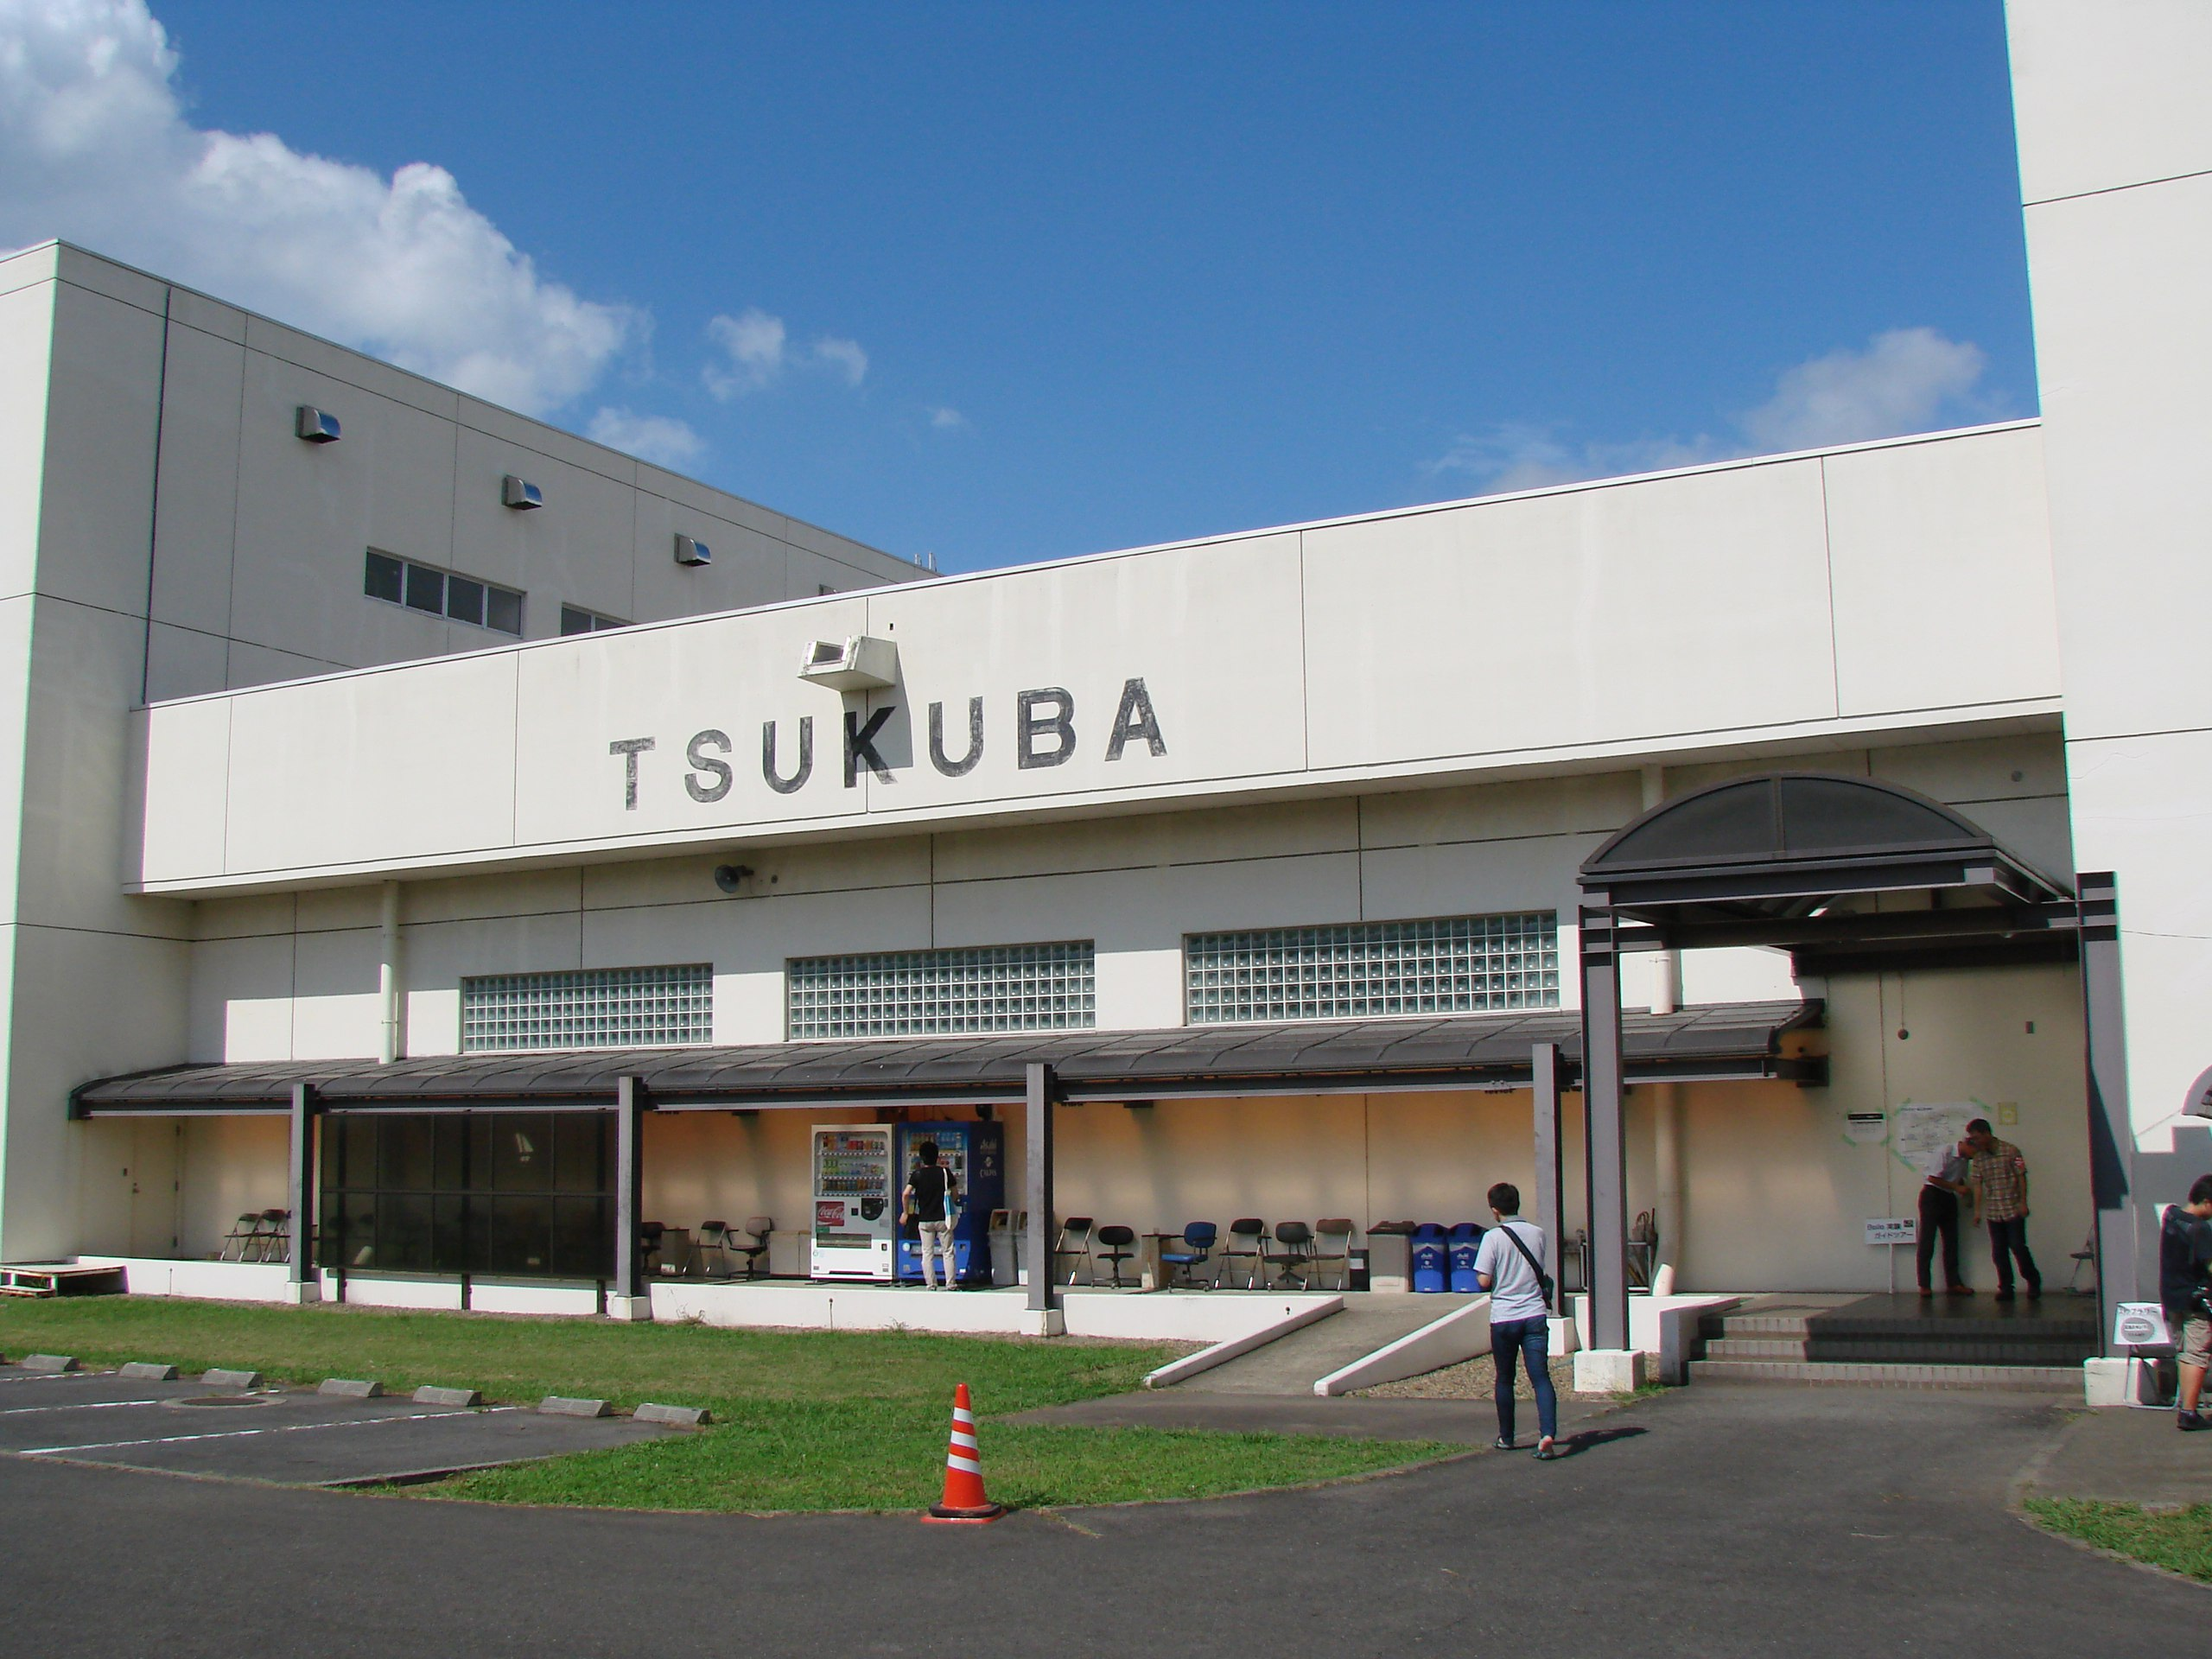
\includegraphics[width=0.7\textwidth]{tsukuba}
        \end{centering}
    \end{figure}
\end{frame}
\begin{frame}
    \frametitle{Детектор Белль 2 под землёй}
    \begin{figure}
        \begin{centering}
            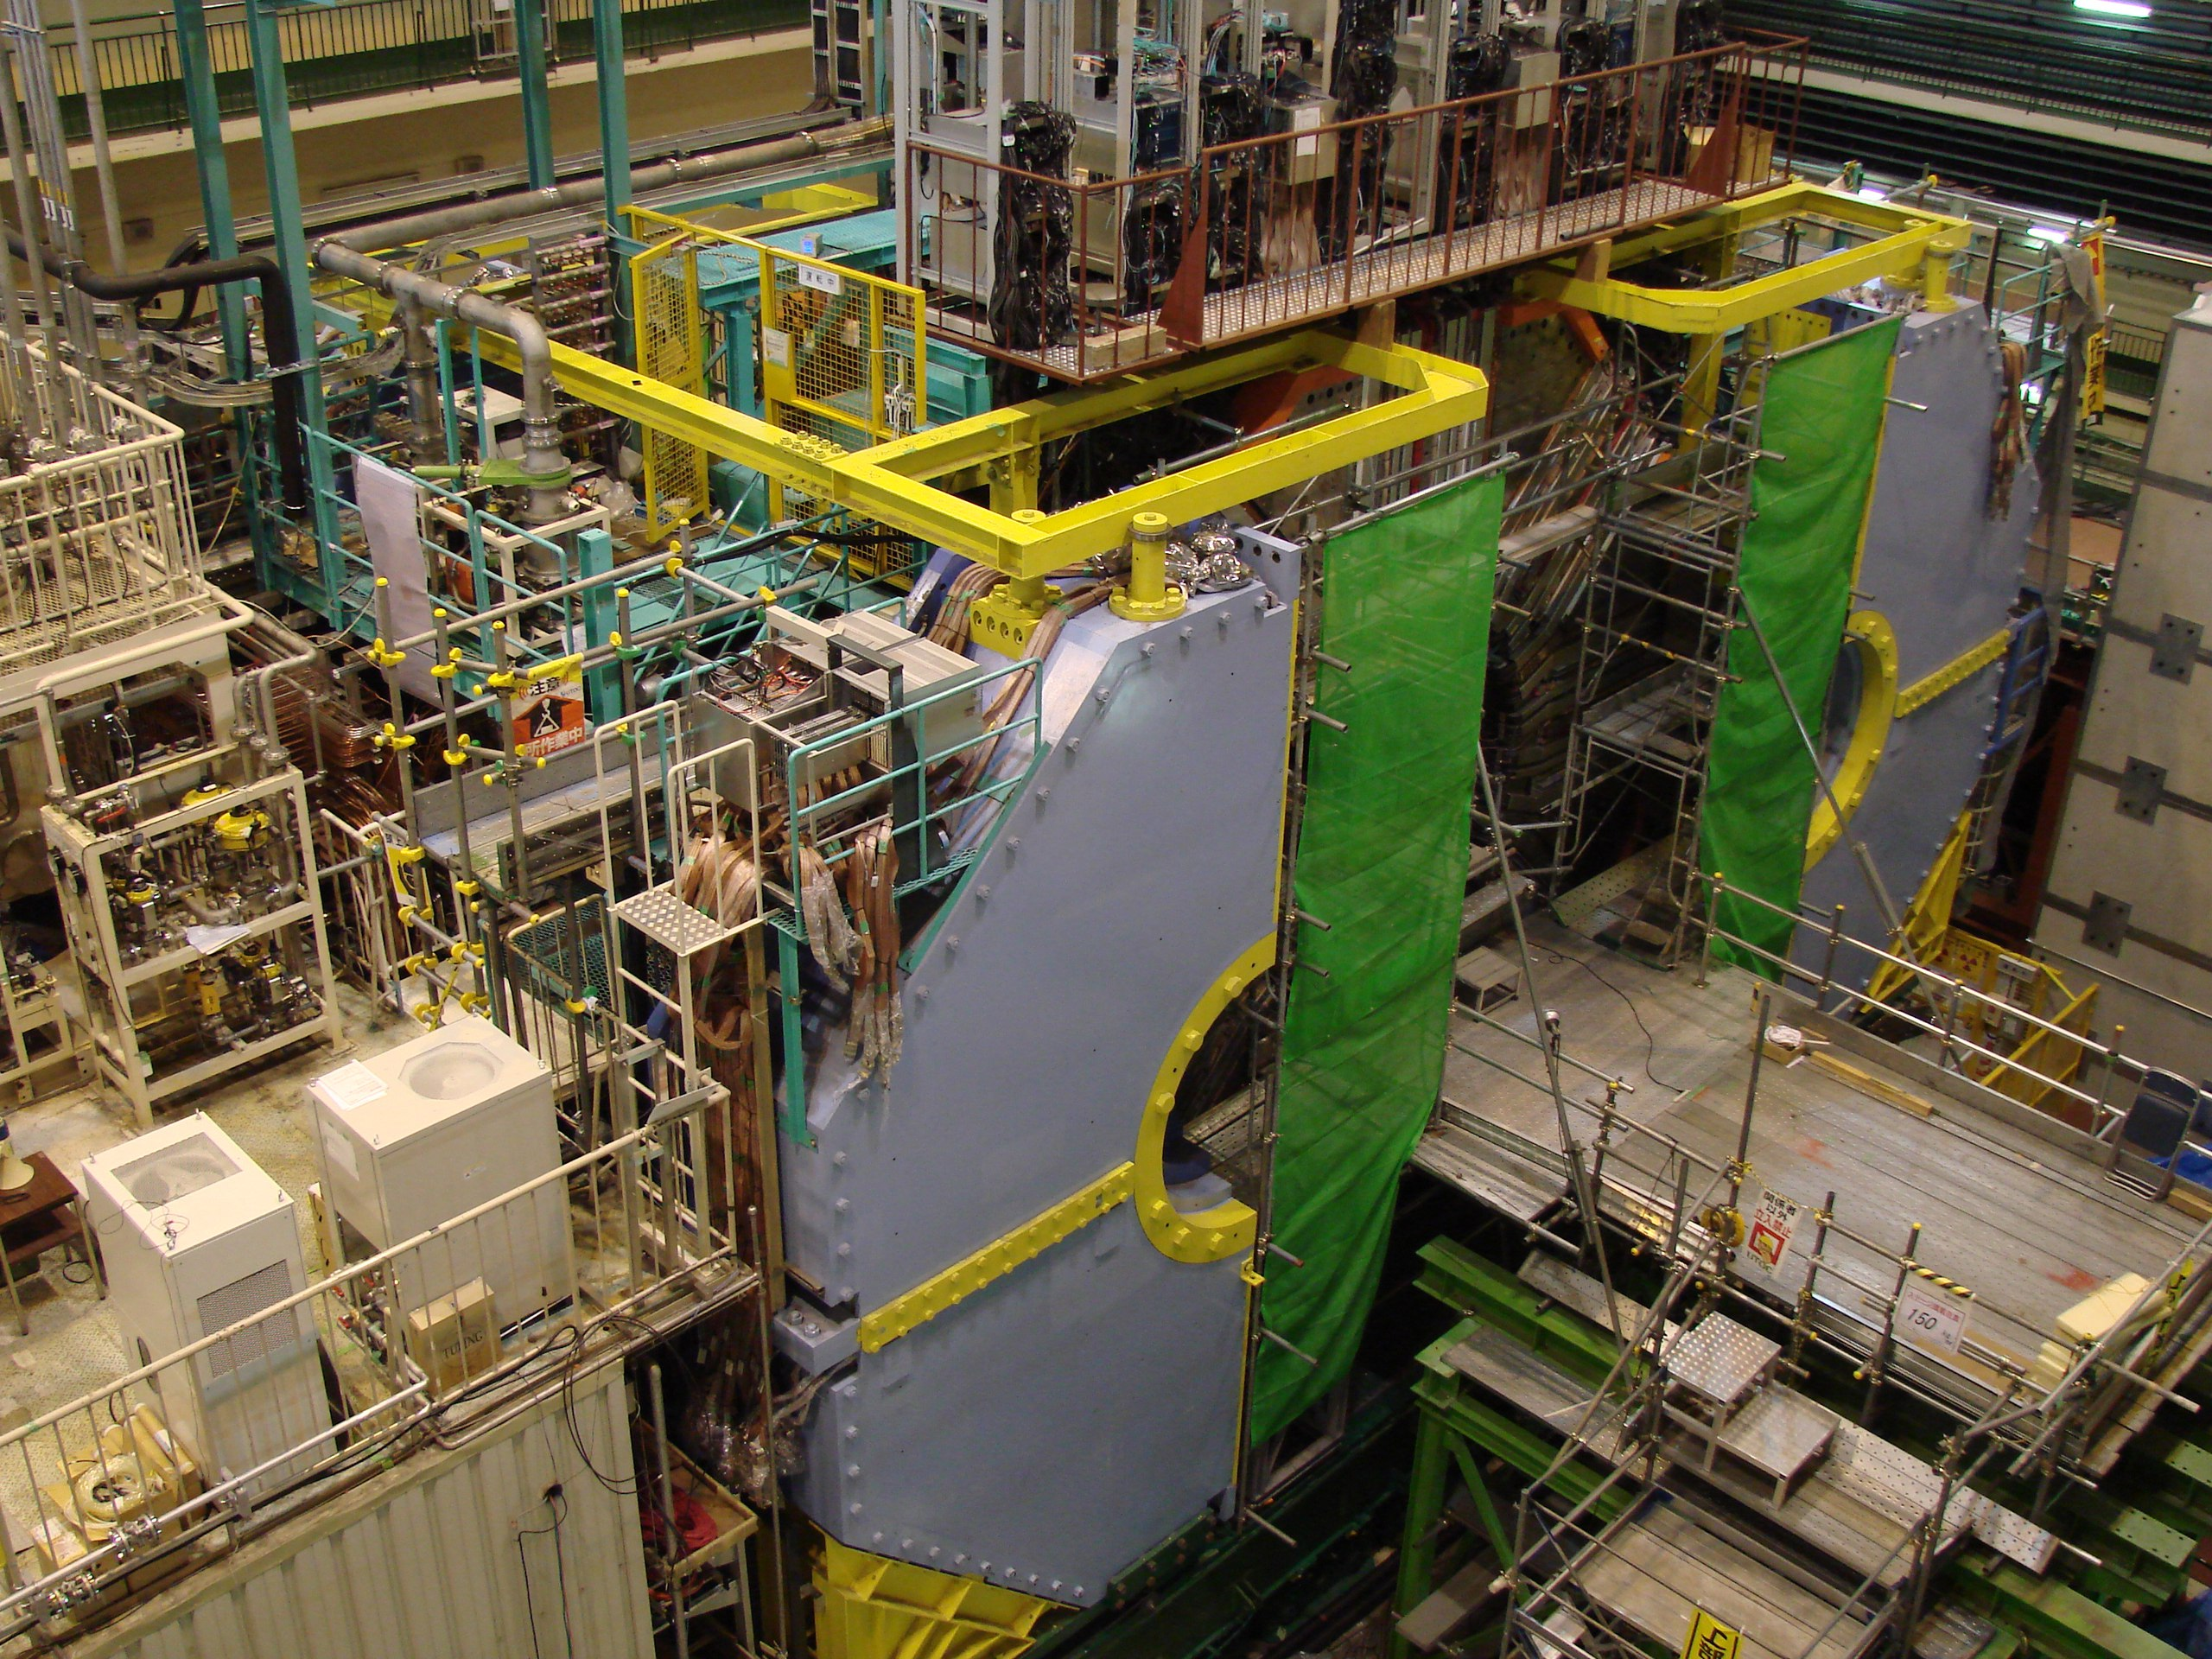
\includegraphics[width=0.7\textwidth]{belle2}
        \end{centering}
    \end{figure}
\end{frame}
\begin{frame}
    \frametitle{Детектор Белль 2 под землёй}
    \begin{figure}
        \begin{centering}
            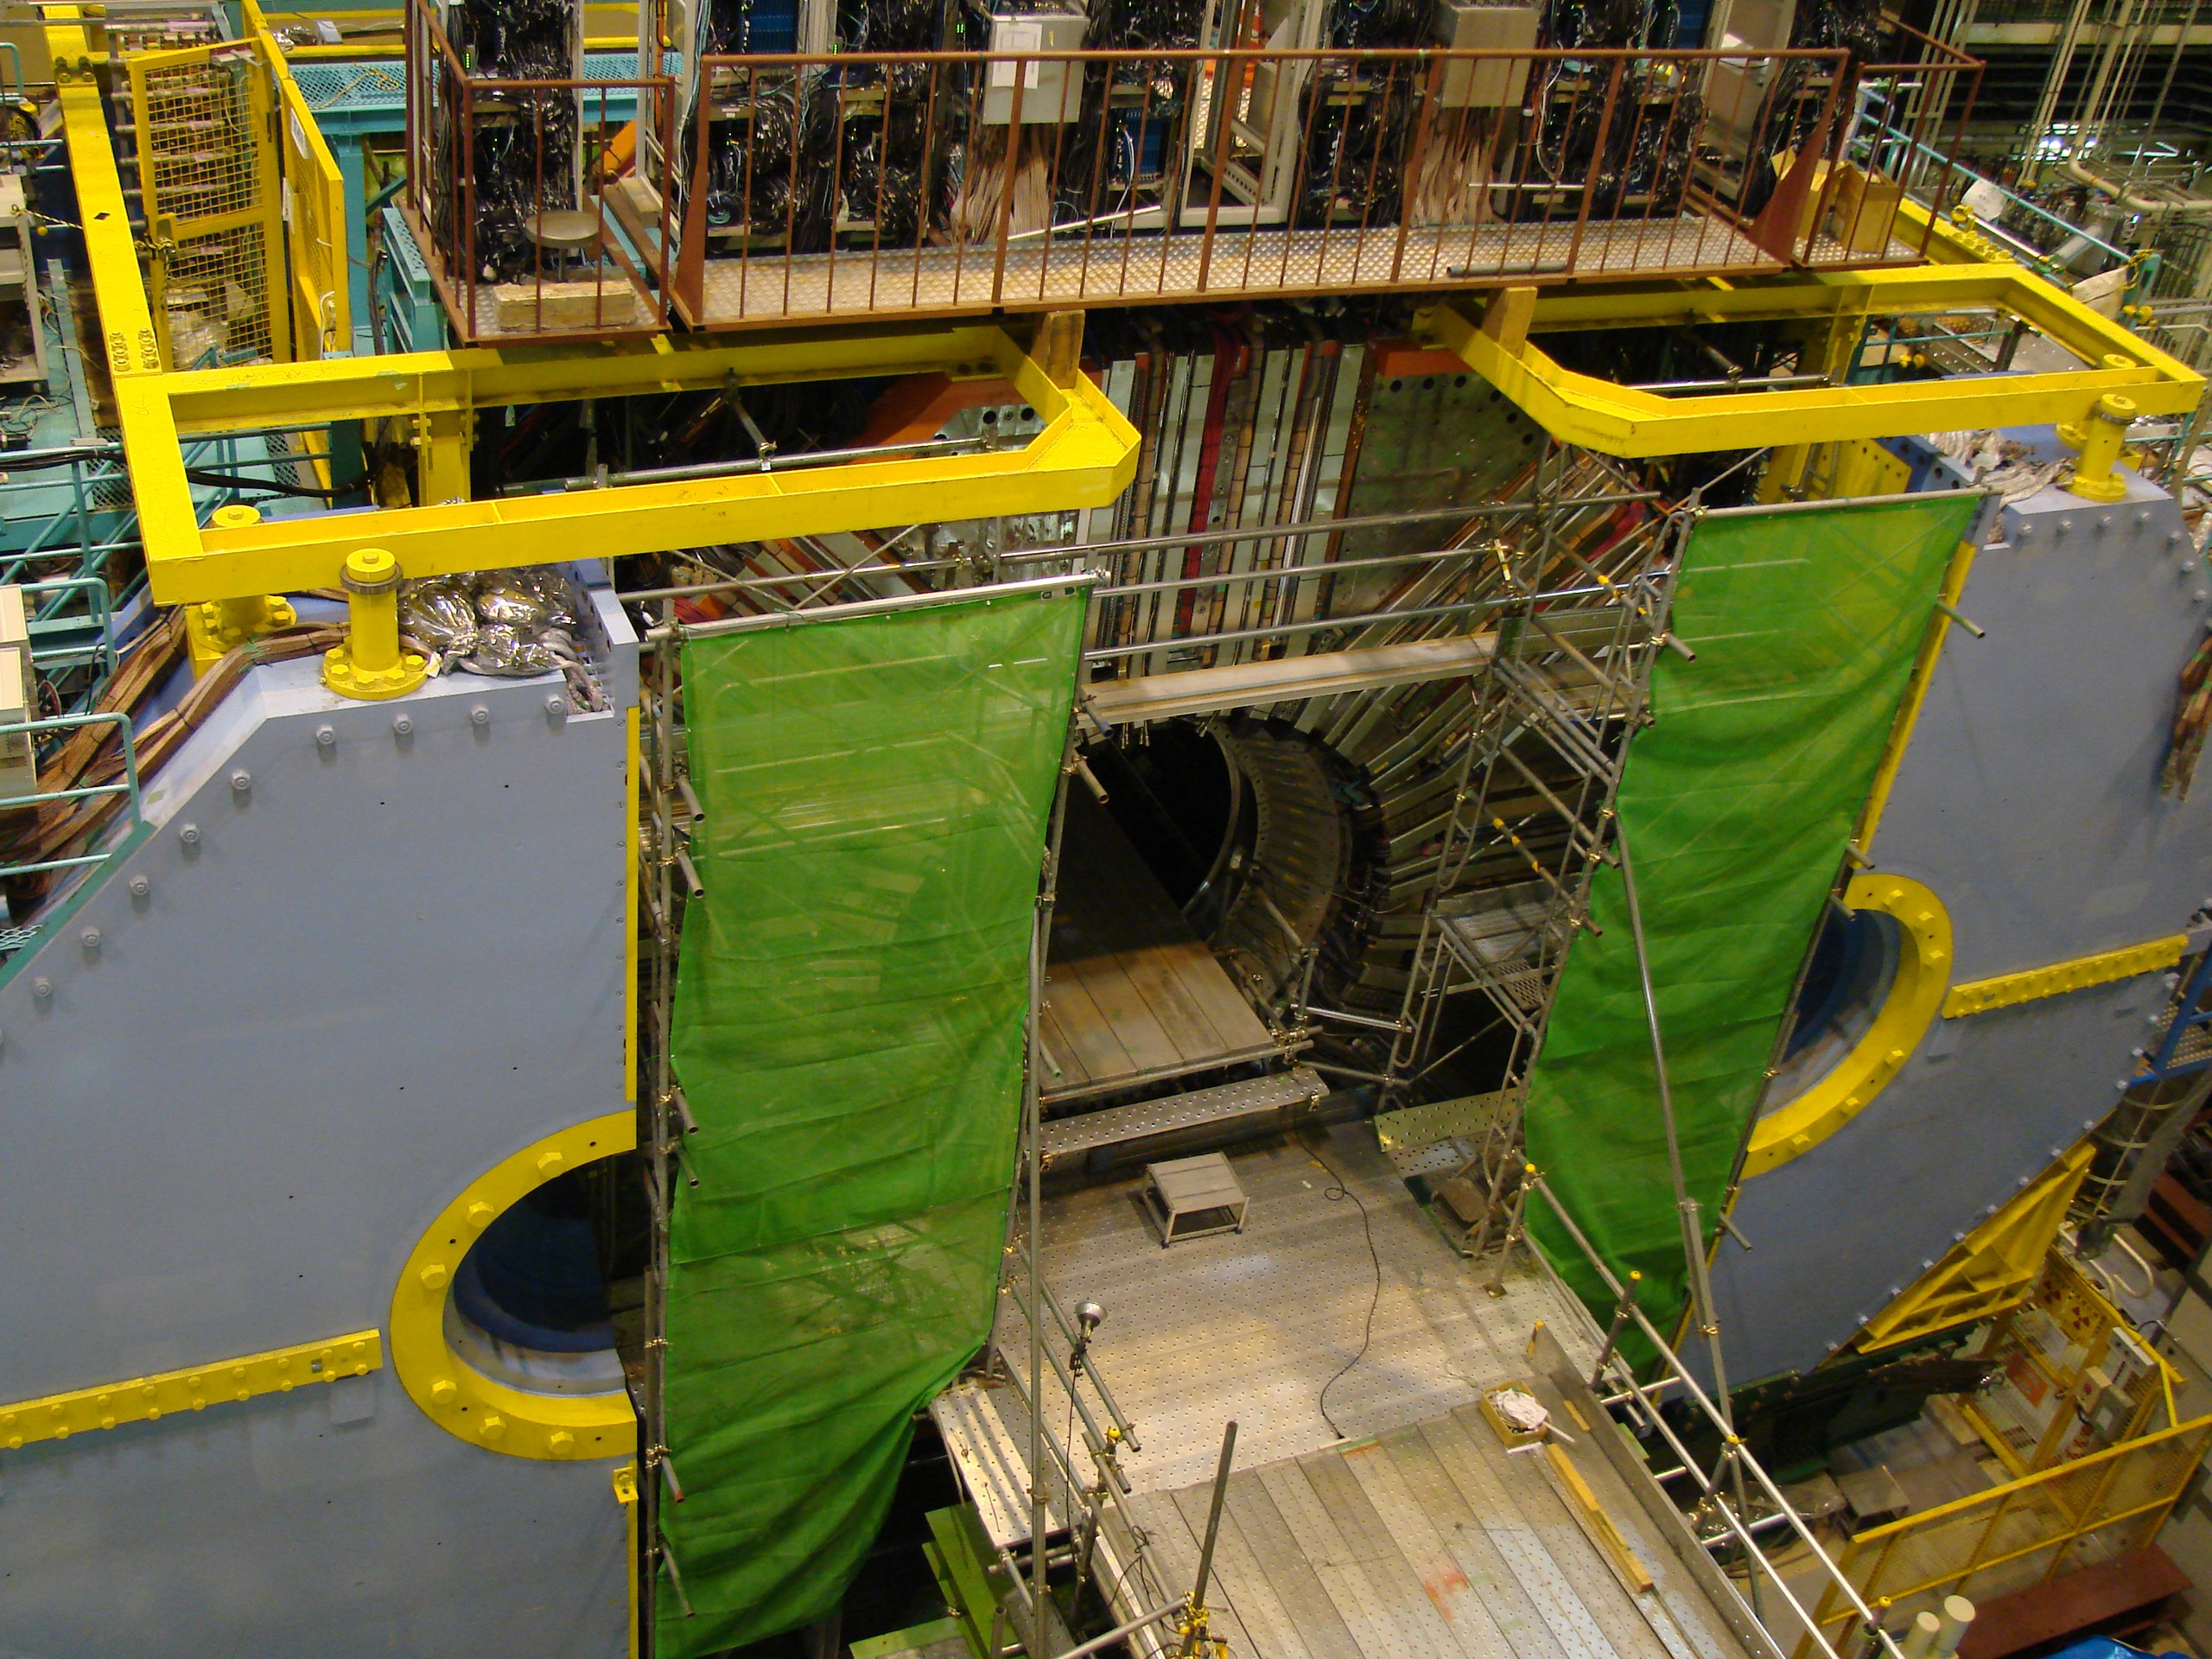
\includegraphics[width=0.7\textwidth]{belle2center}
        \end{centering}
    \end{figure}
\end{frame}
\begin{frame}
    \begin{figure}
        \begin{centering}
            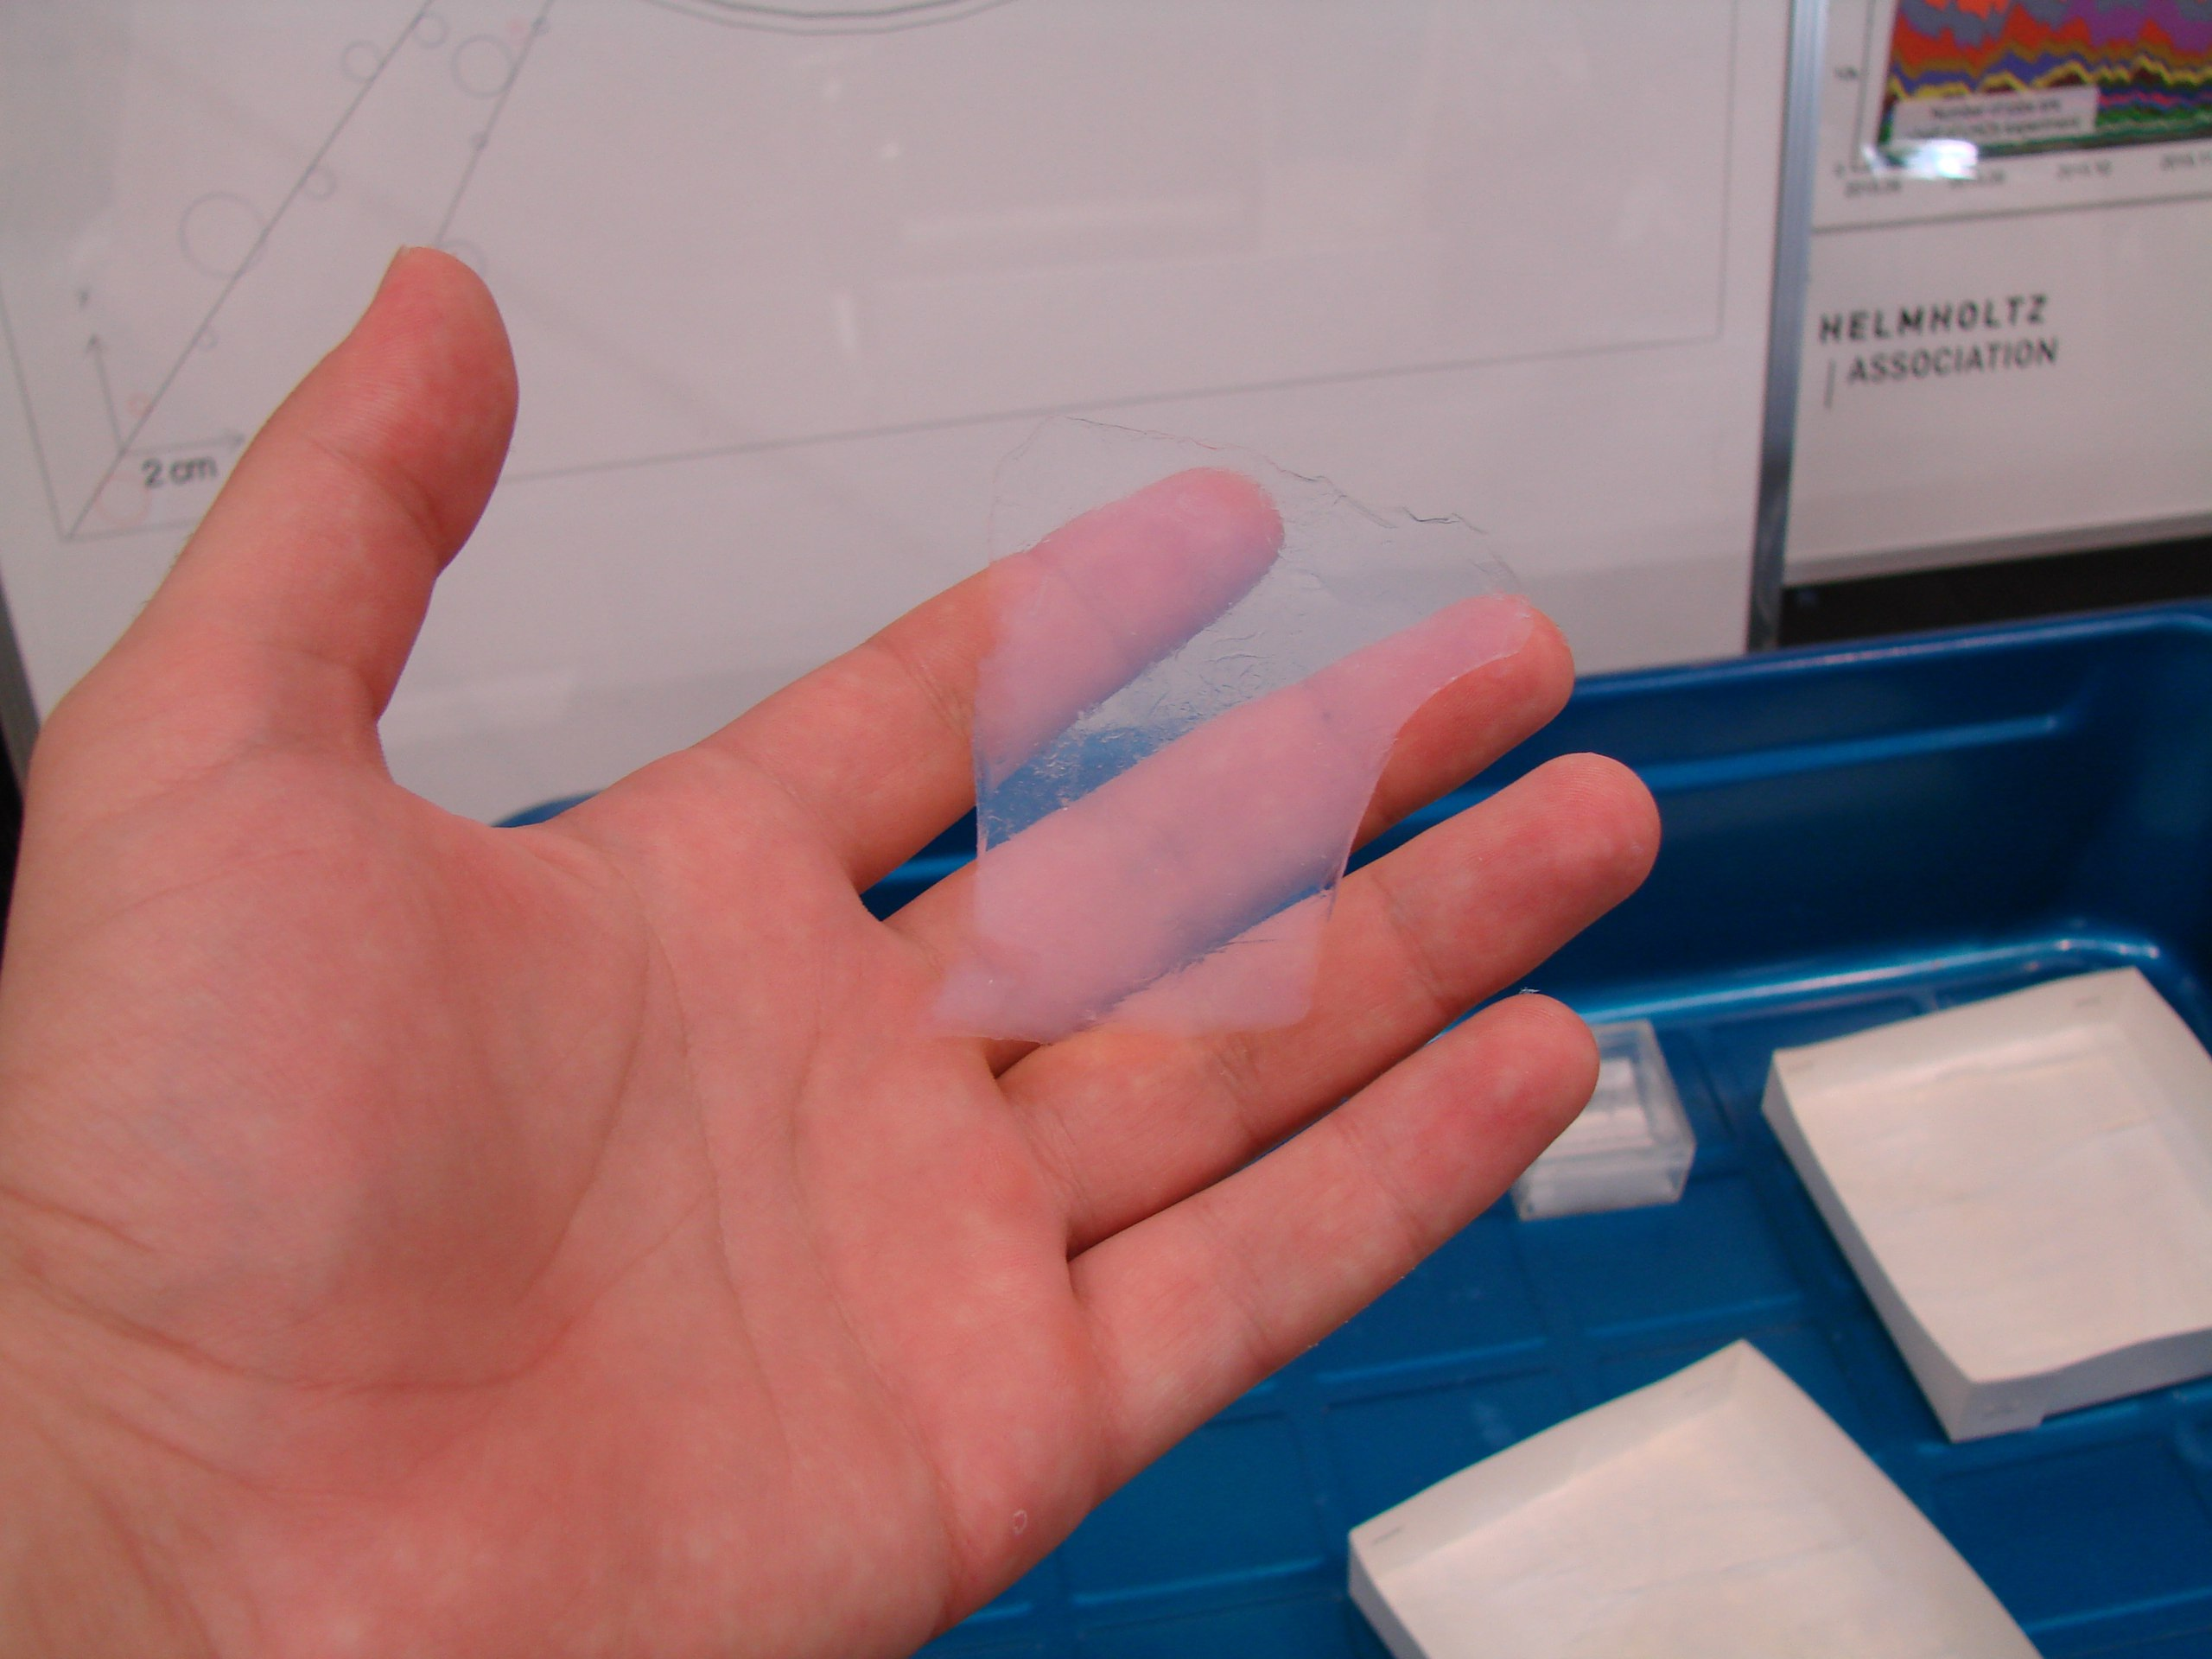
\includegraphics[width=0.7\textwidth]{aerogel}
        \end{centering}
    \end{figure}
\end{frame}
\begin{frame}
    \begin{figure}
        \begin{centering}
            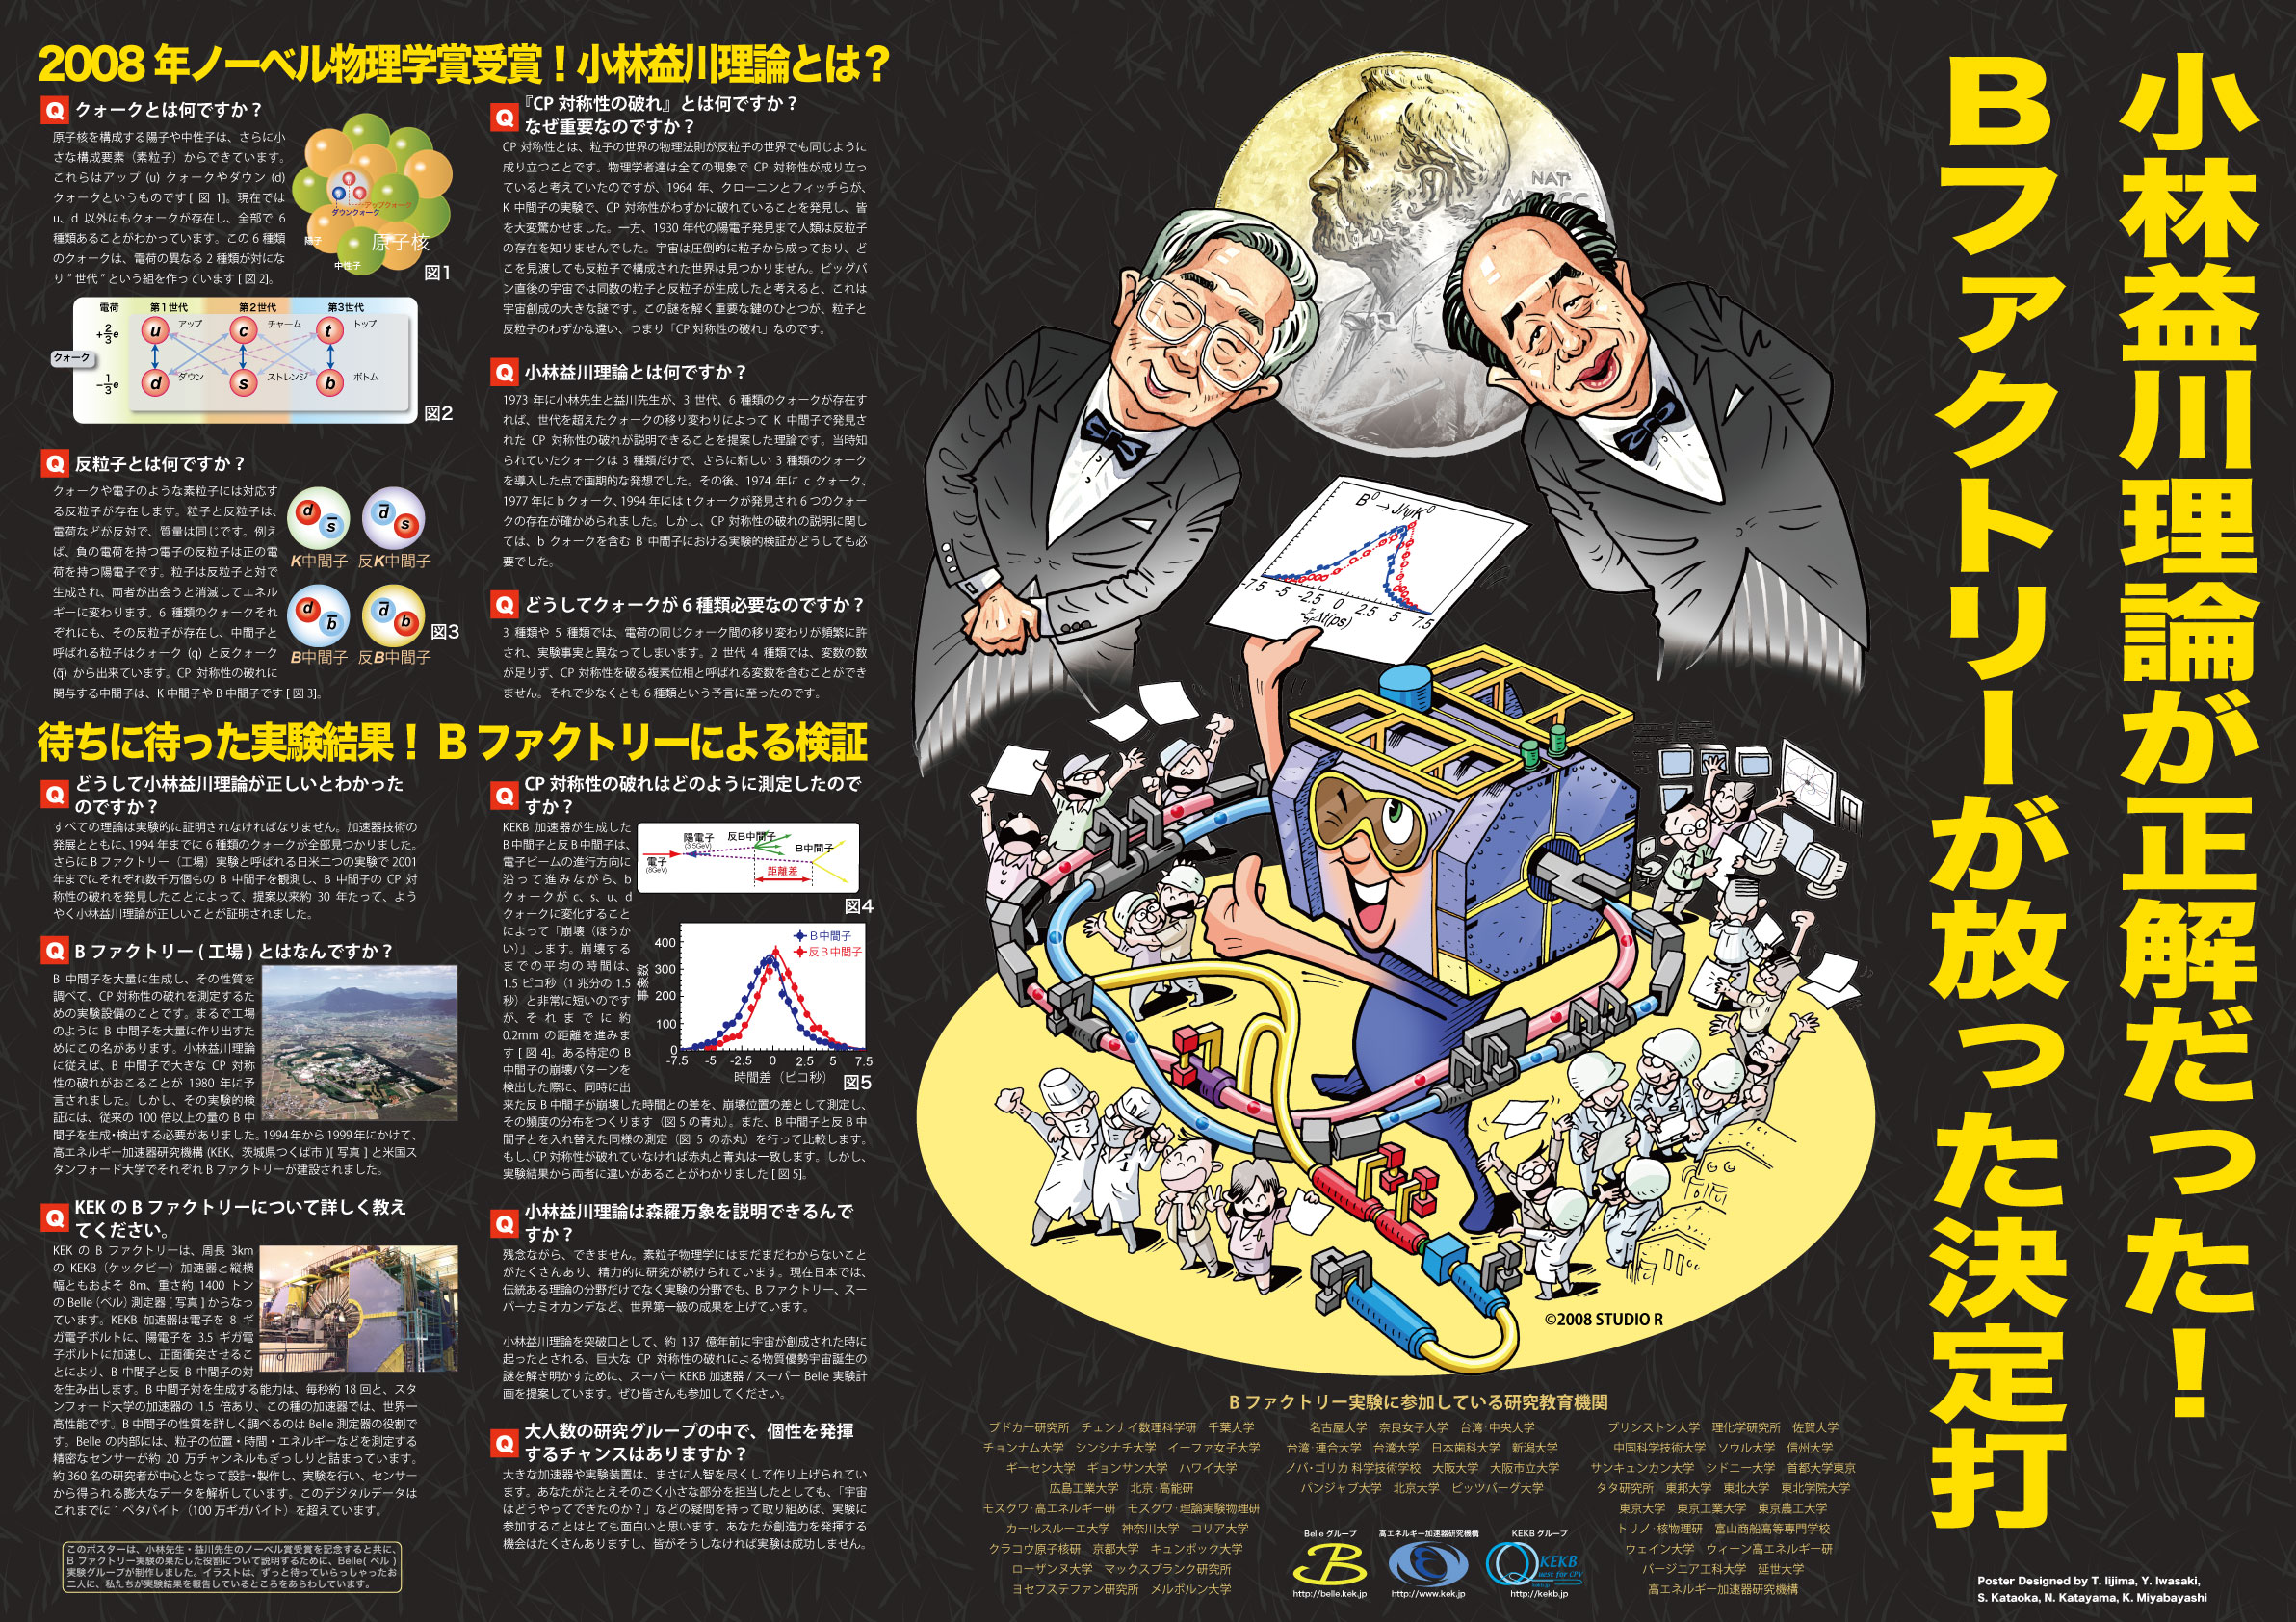
\includegraphics[width=0.95\textwidth]{KM-poster}
        \end{centering}
    \end{figure}
\end{frame}



\subsection{LHC}
\begin{frame}
    {\LARGE Большой адронный коллайдер}
\end{frame}
\begin{frame}
    \frametitle{Большой адронный коллайдер где-то рядом}
    \begin{figure}
        \begin{centering}
            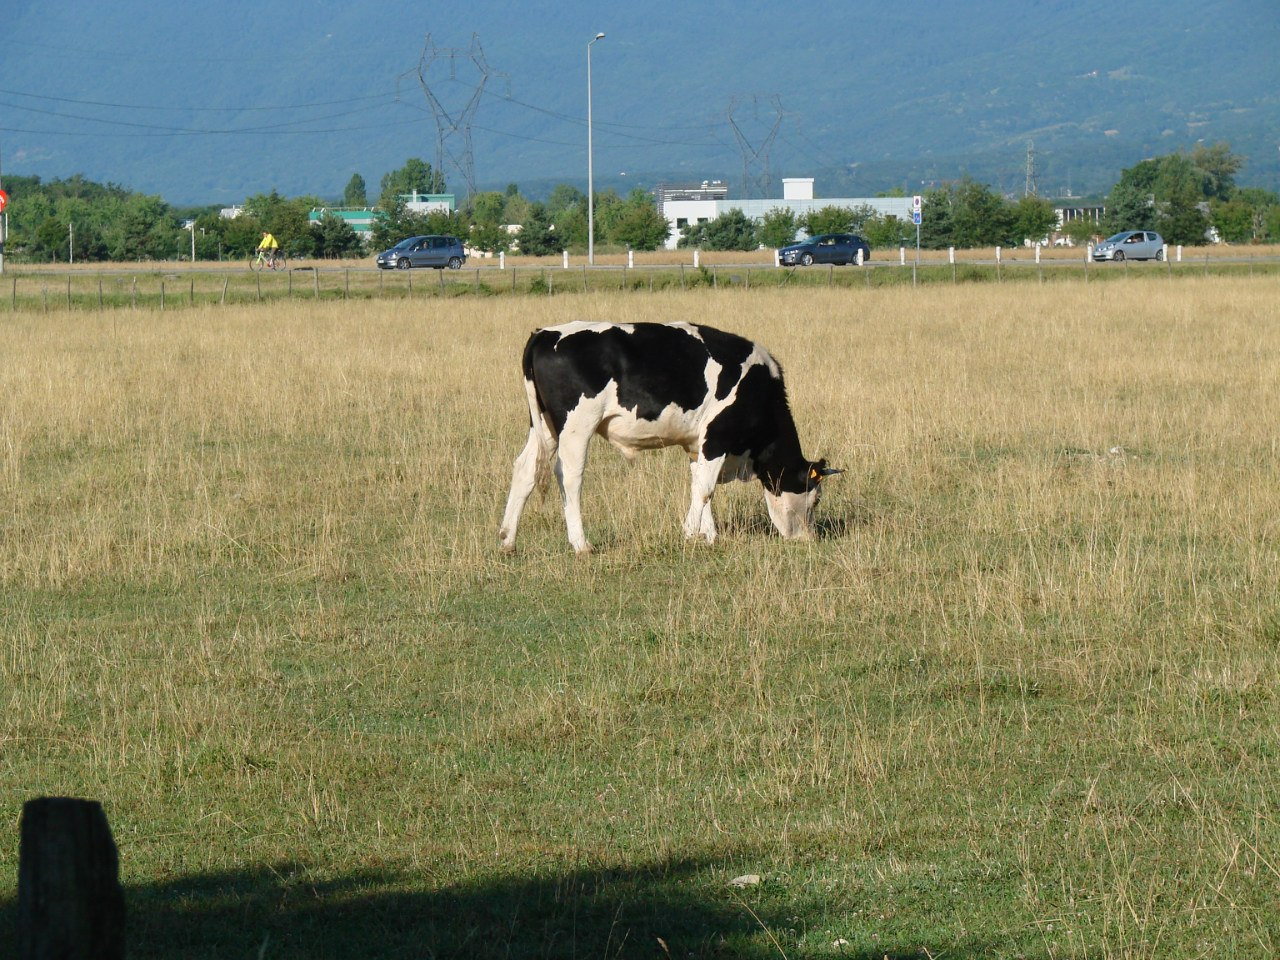
\includegraphics[width=0.7\textwidth]{lhc-top}
        \end{centering}
    \end{figure}
\end{frame}
\begin{frame}
    \begin{figure}
        \begin{centering}
            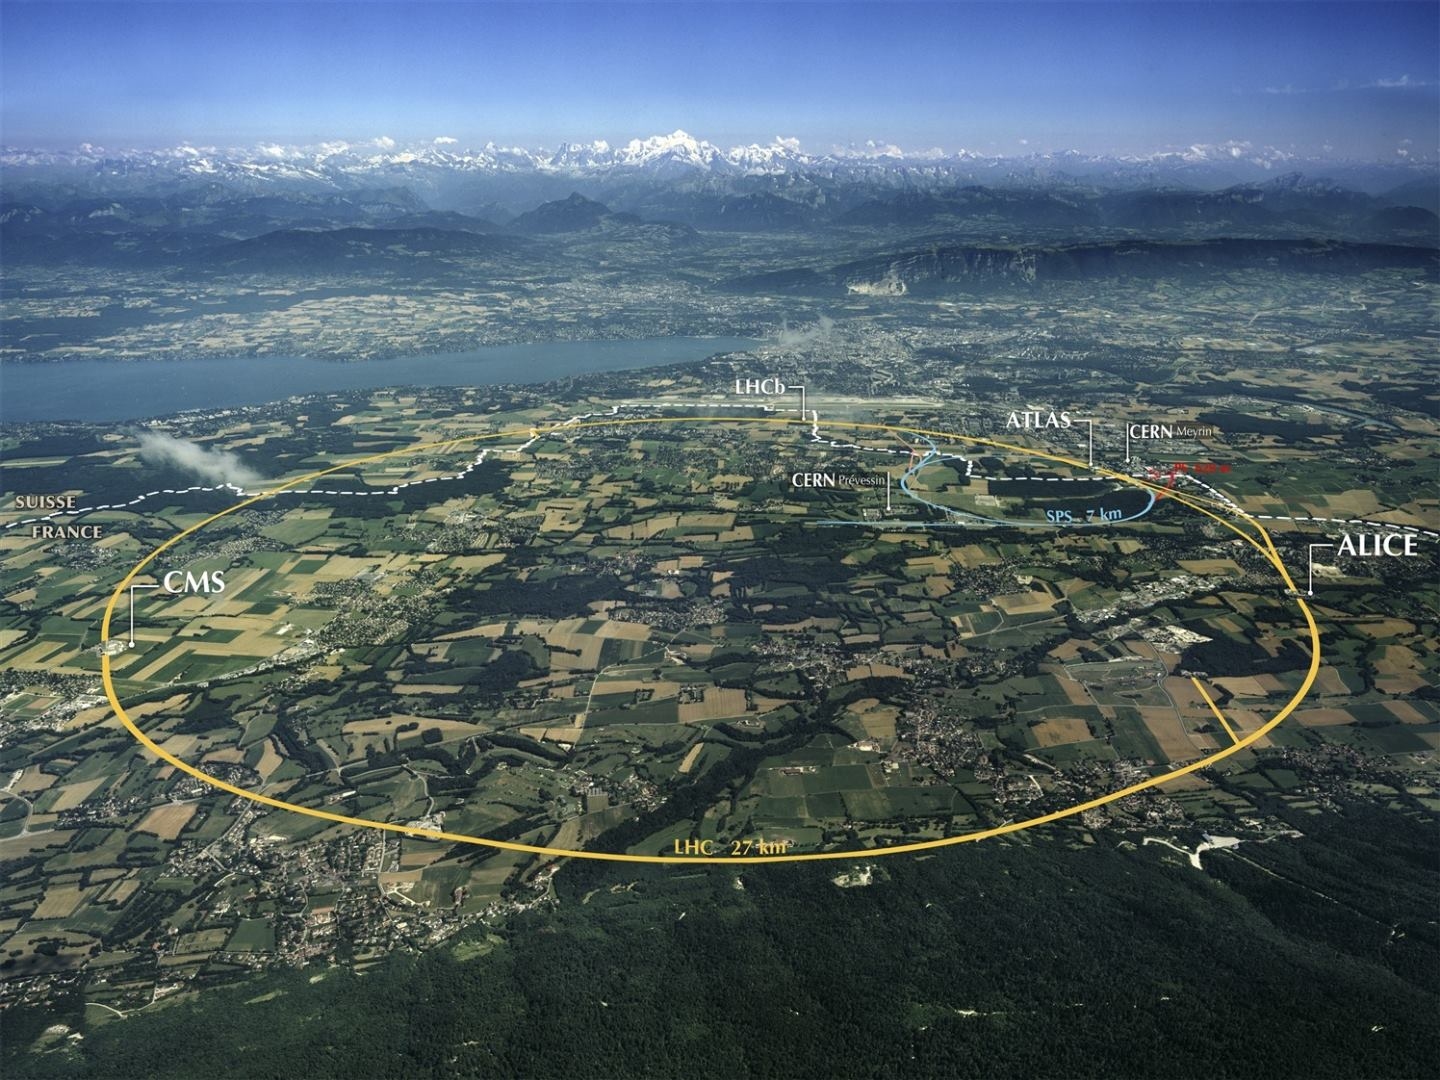
\includegraphics[width=0.7\textwidth]{lhc}
        \end{centering}
    \end{figure}
\end{frame}
\begin{frame}
    \begin{figure}
        \begin{centering}
            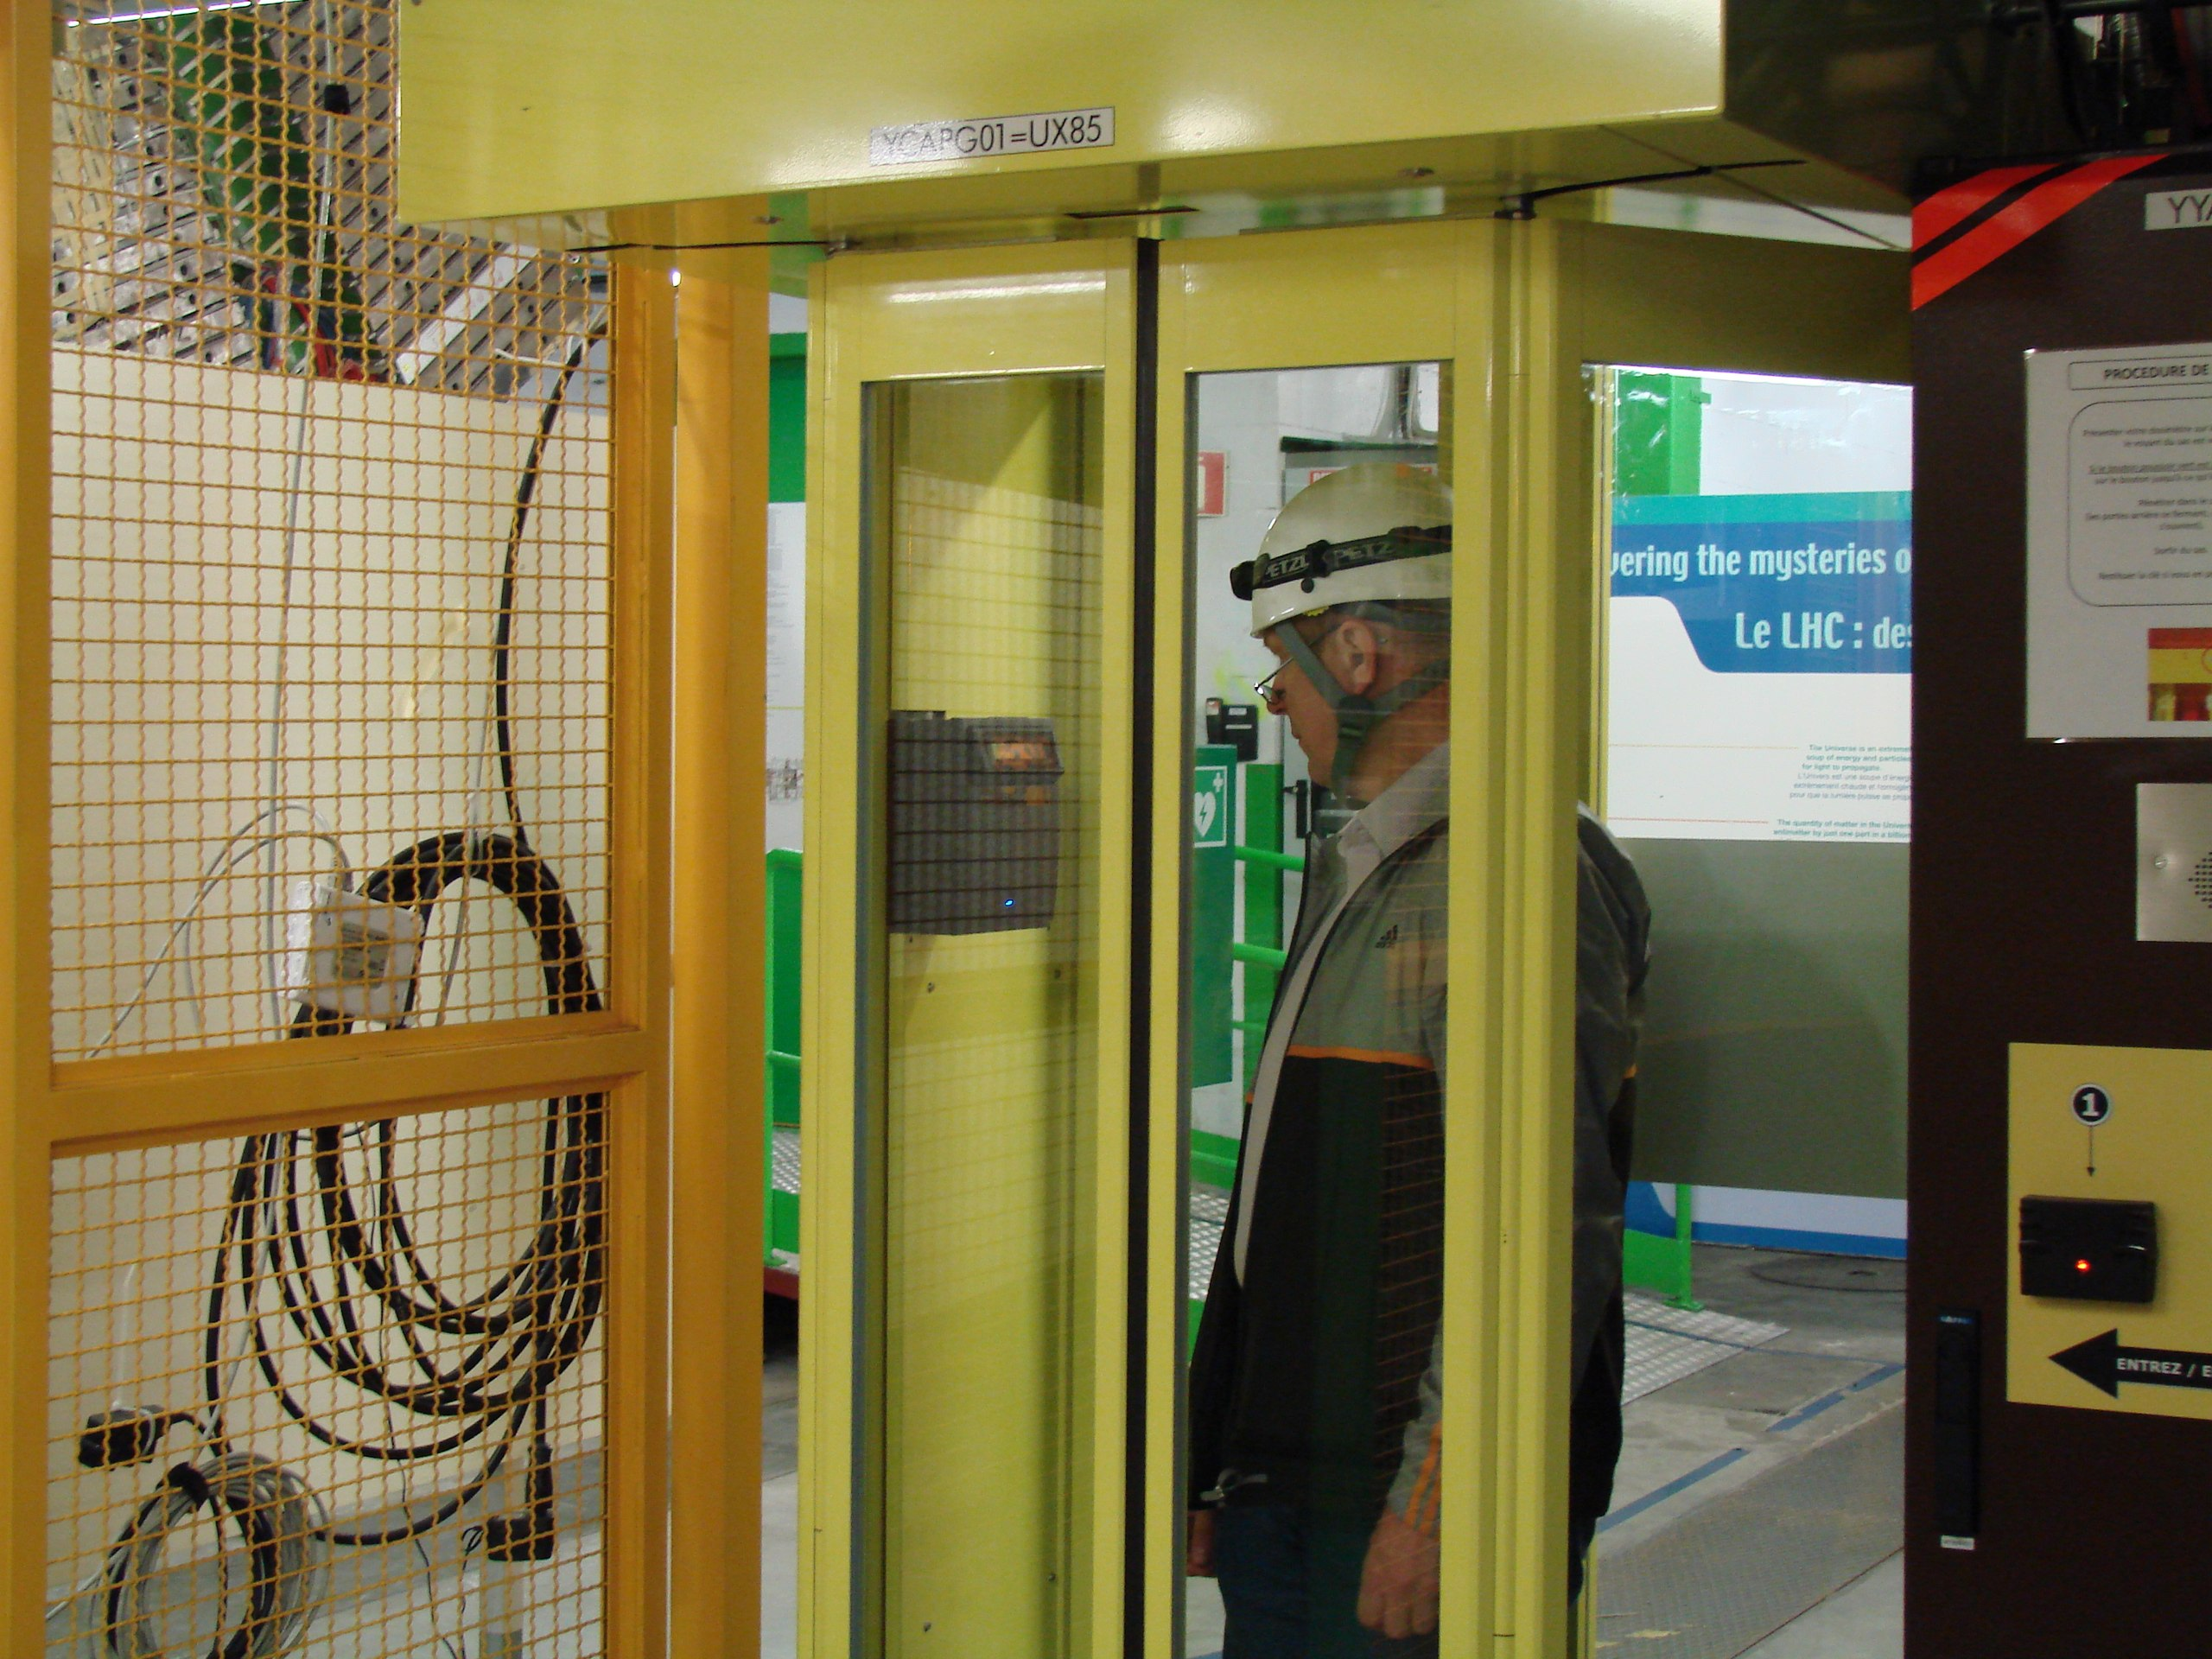
\includegraphics[width=0.7\textwidth]{eye-scan}
        \end{centering}
    \end{figure}
\end{frame}
\begin{frame}
    \frametitle{Транспорт для коллайдера}
    \begin{figure}
        \begin{centering}
            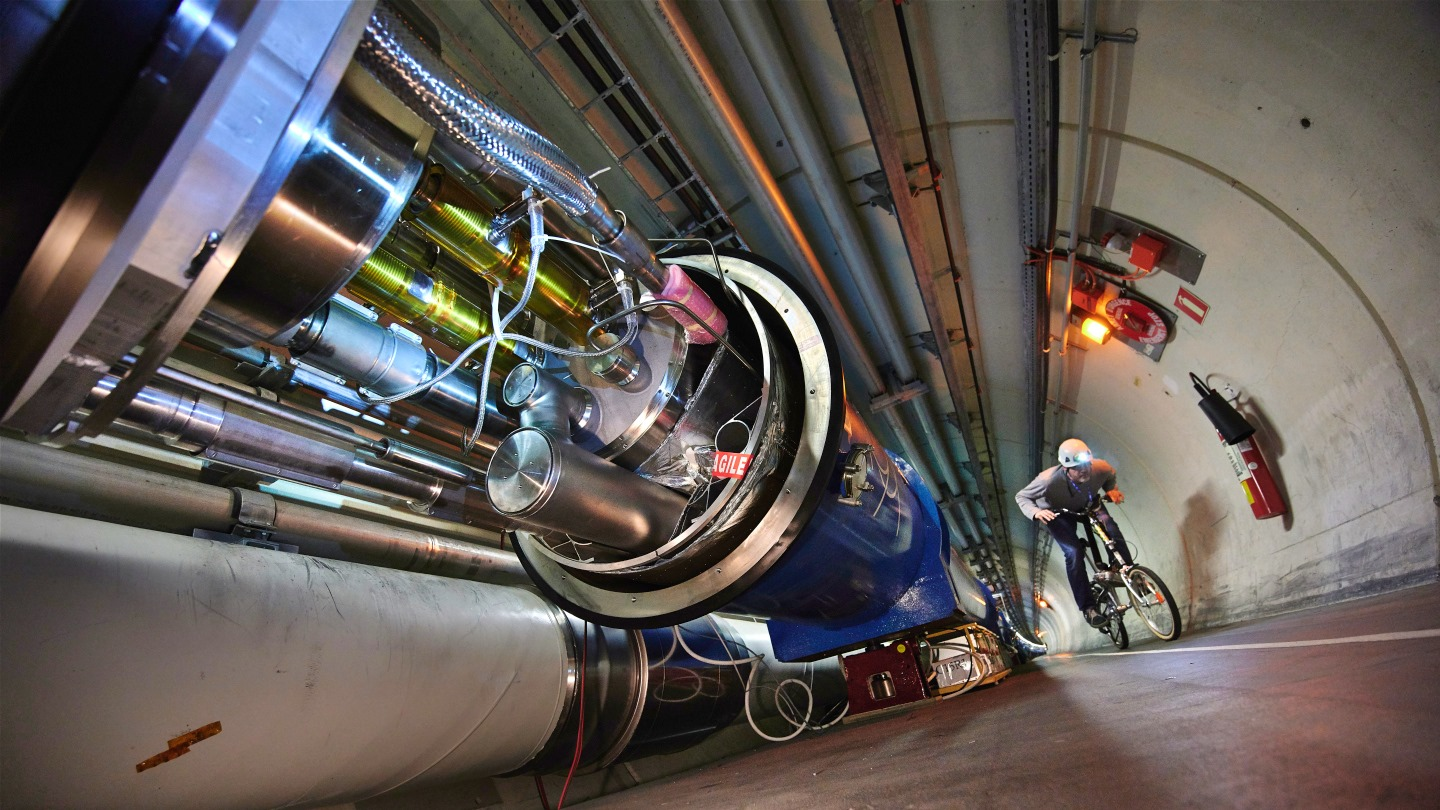
\includegraphics[width=0.85\textwidth]{lhc-bike}
        \end{centering}
    \end{figure}
\end{frame}
\begin{frame}
    \begin{figure}
        \begin{centering}
            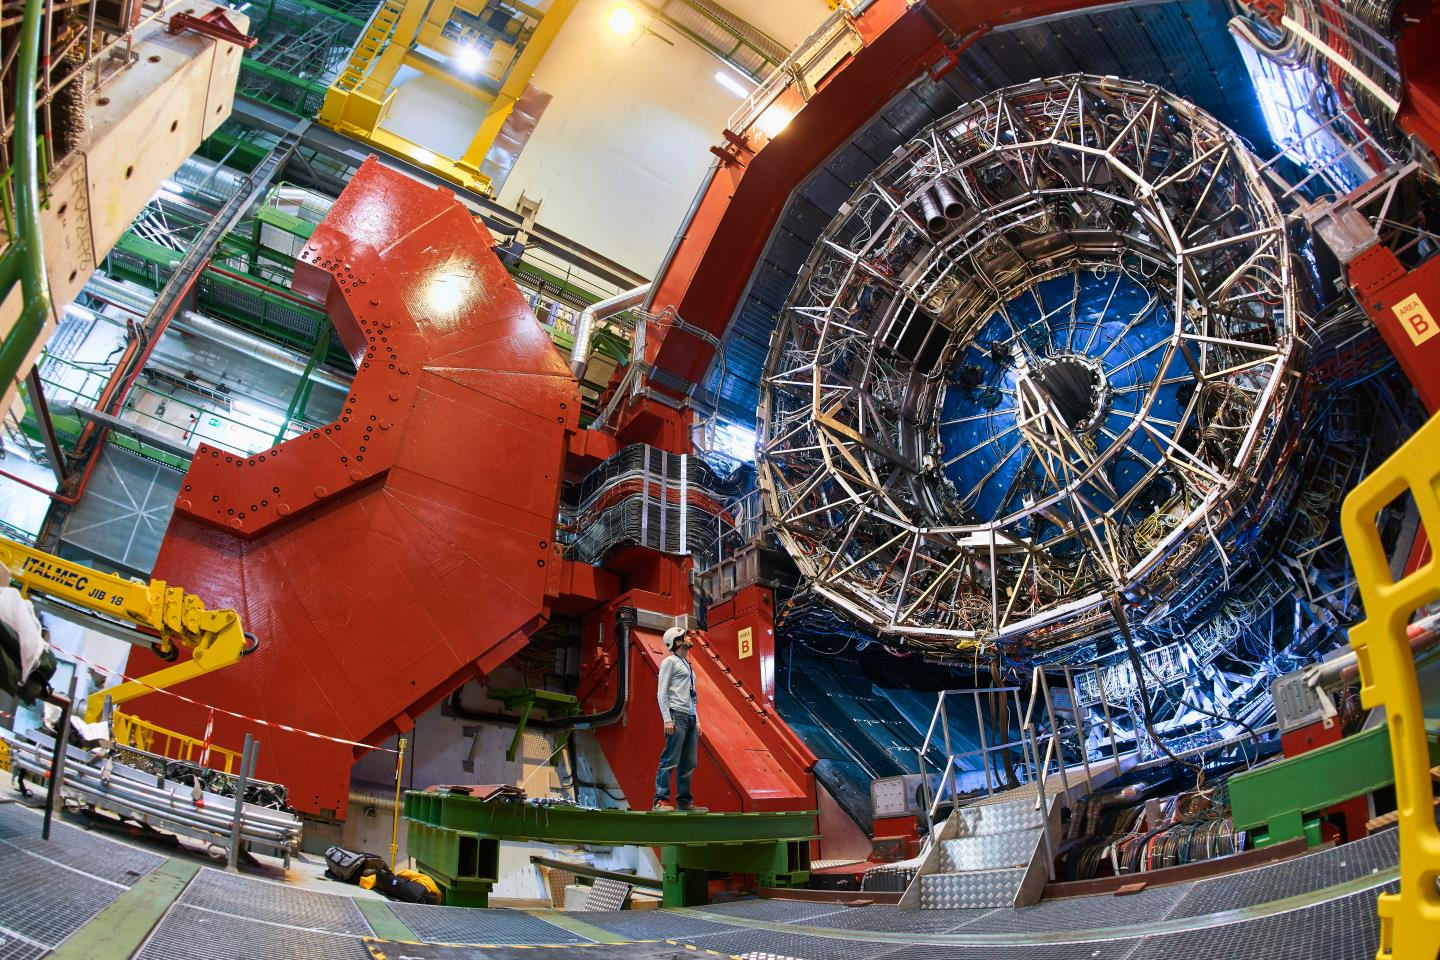
\includegraphics[width=0.8\textwidth]{alice}
        \end{centering}
    \end{figure}
\end{frame}
\begin{frame}
    \begin{figure}
        \begin{centering}
            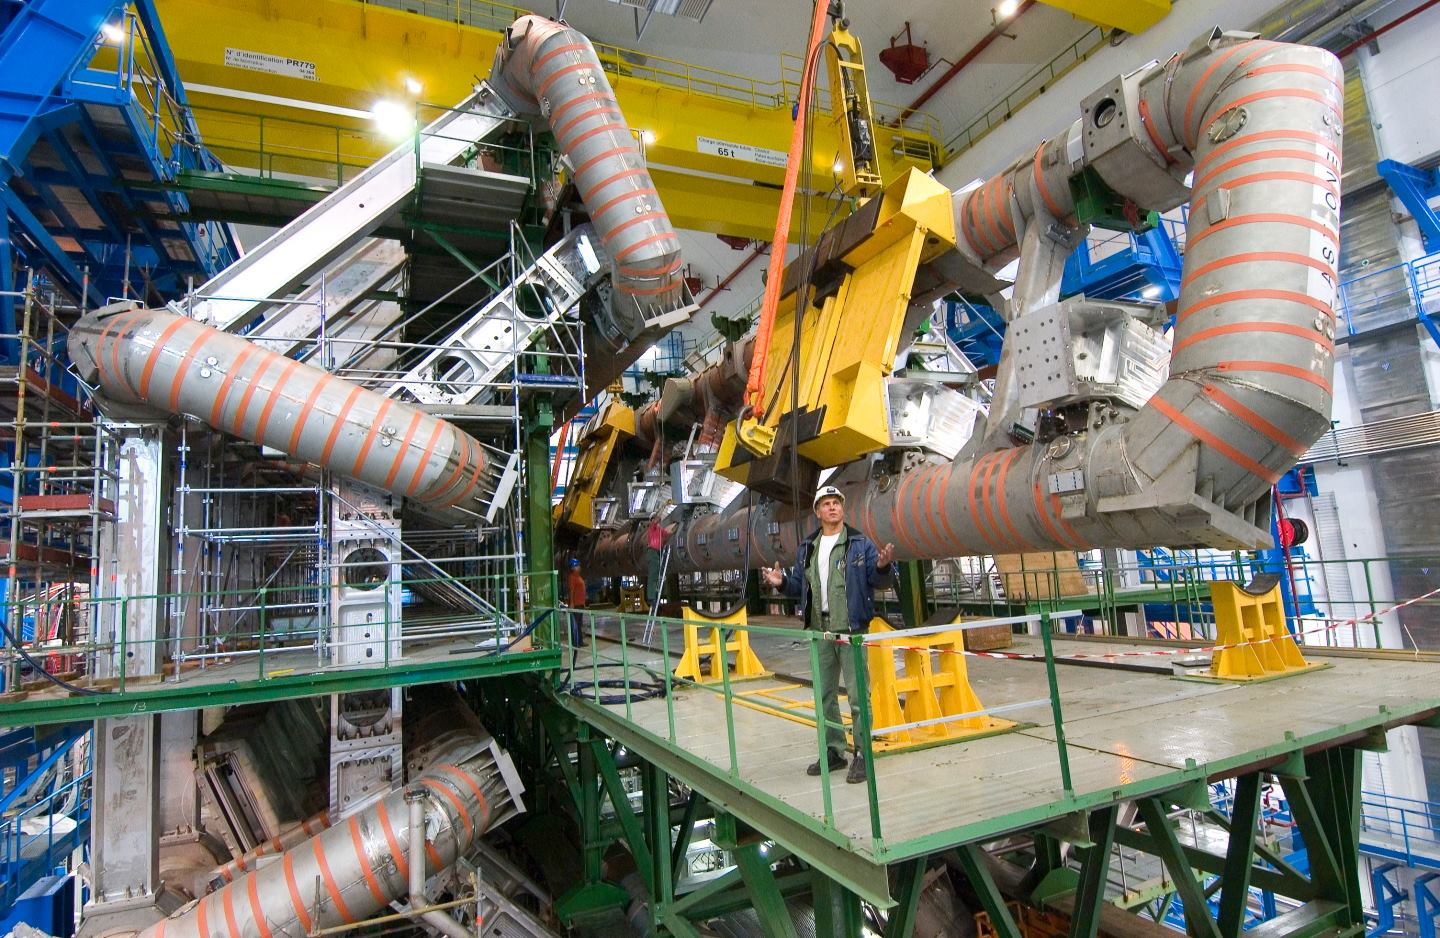
\includegraphics[width=0.8\textwidth]{atlas}
        \end{centering}
    \end{figure}
\end{frame}
\begin{frame}
    \begin{figure}
        \begin{centering}
            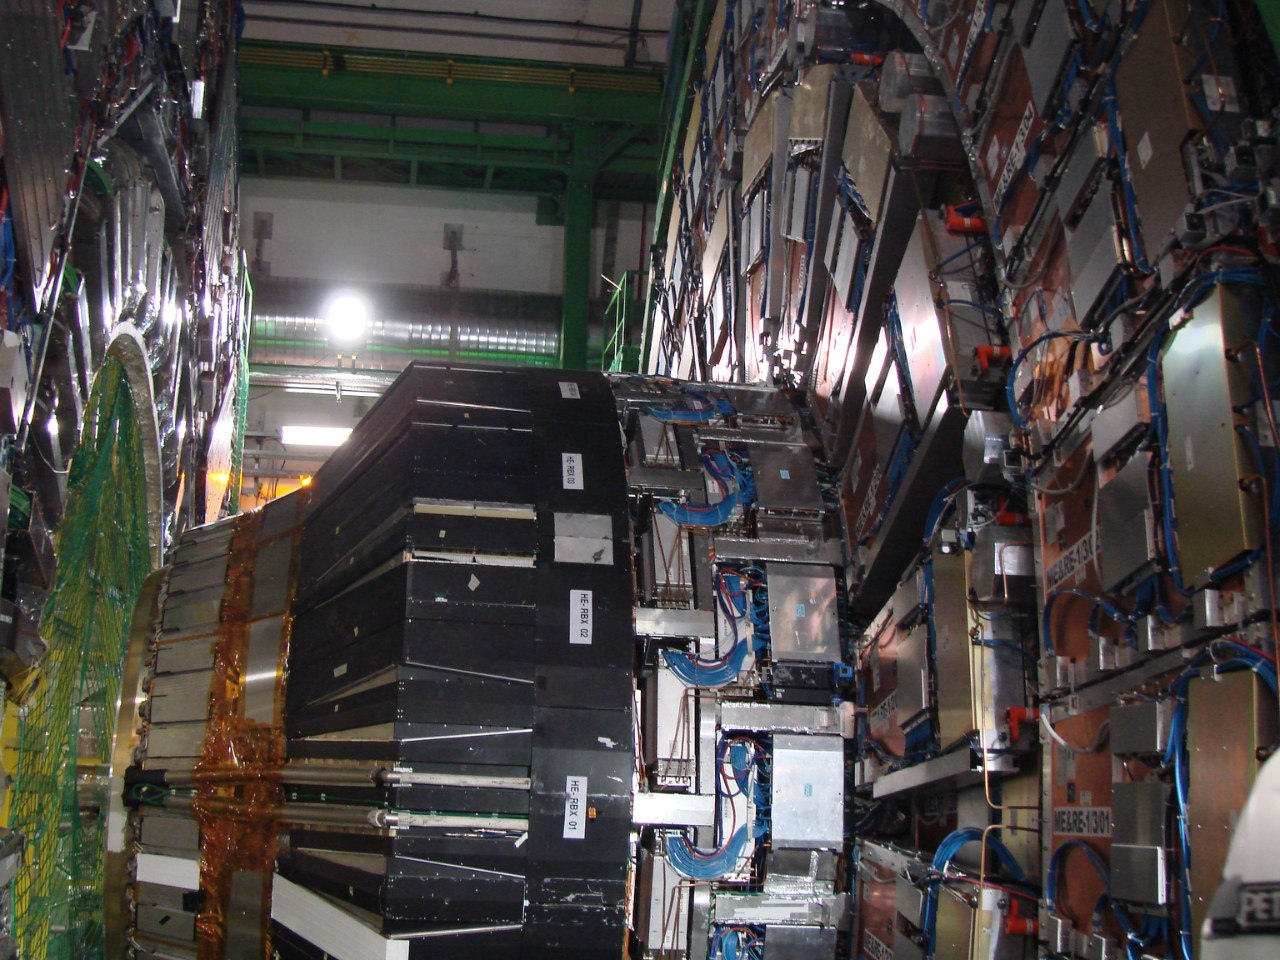
\includegraphics[width=0.8\textwidth]{cms}
        \end{centering}
    \end{figure}
\end{frame}
\begin{frame}
    \begin{figure}
        \begin{centering}
            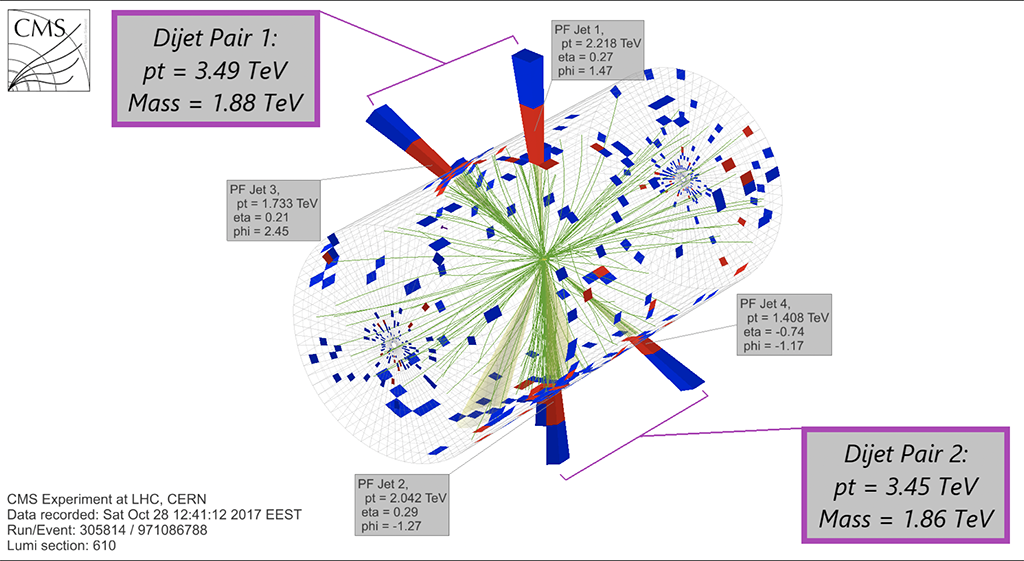
\includegraphics[width=0.9\textwidth]{cms-ed}
        \end{centering}
    \end{figure}
\end{frame}
\begin{frame}
    \begin{figure}
        \begin{centering}
            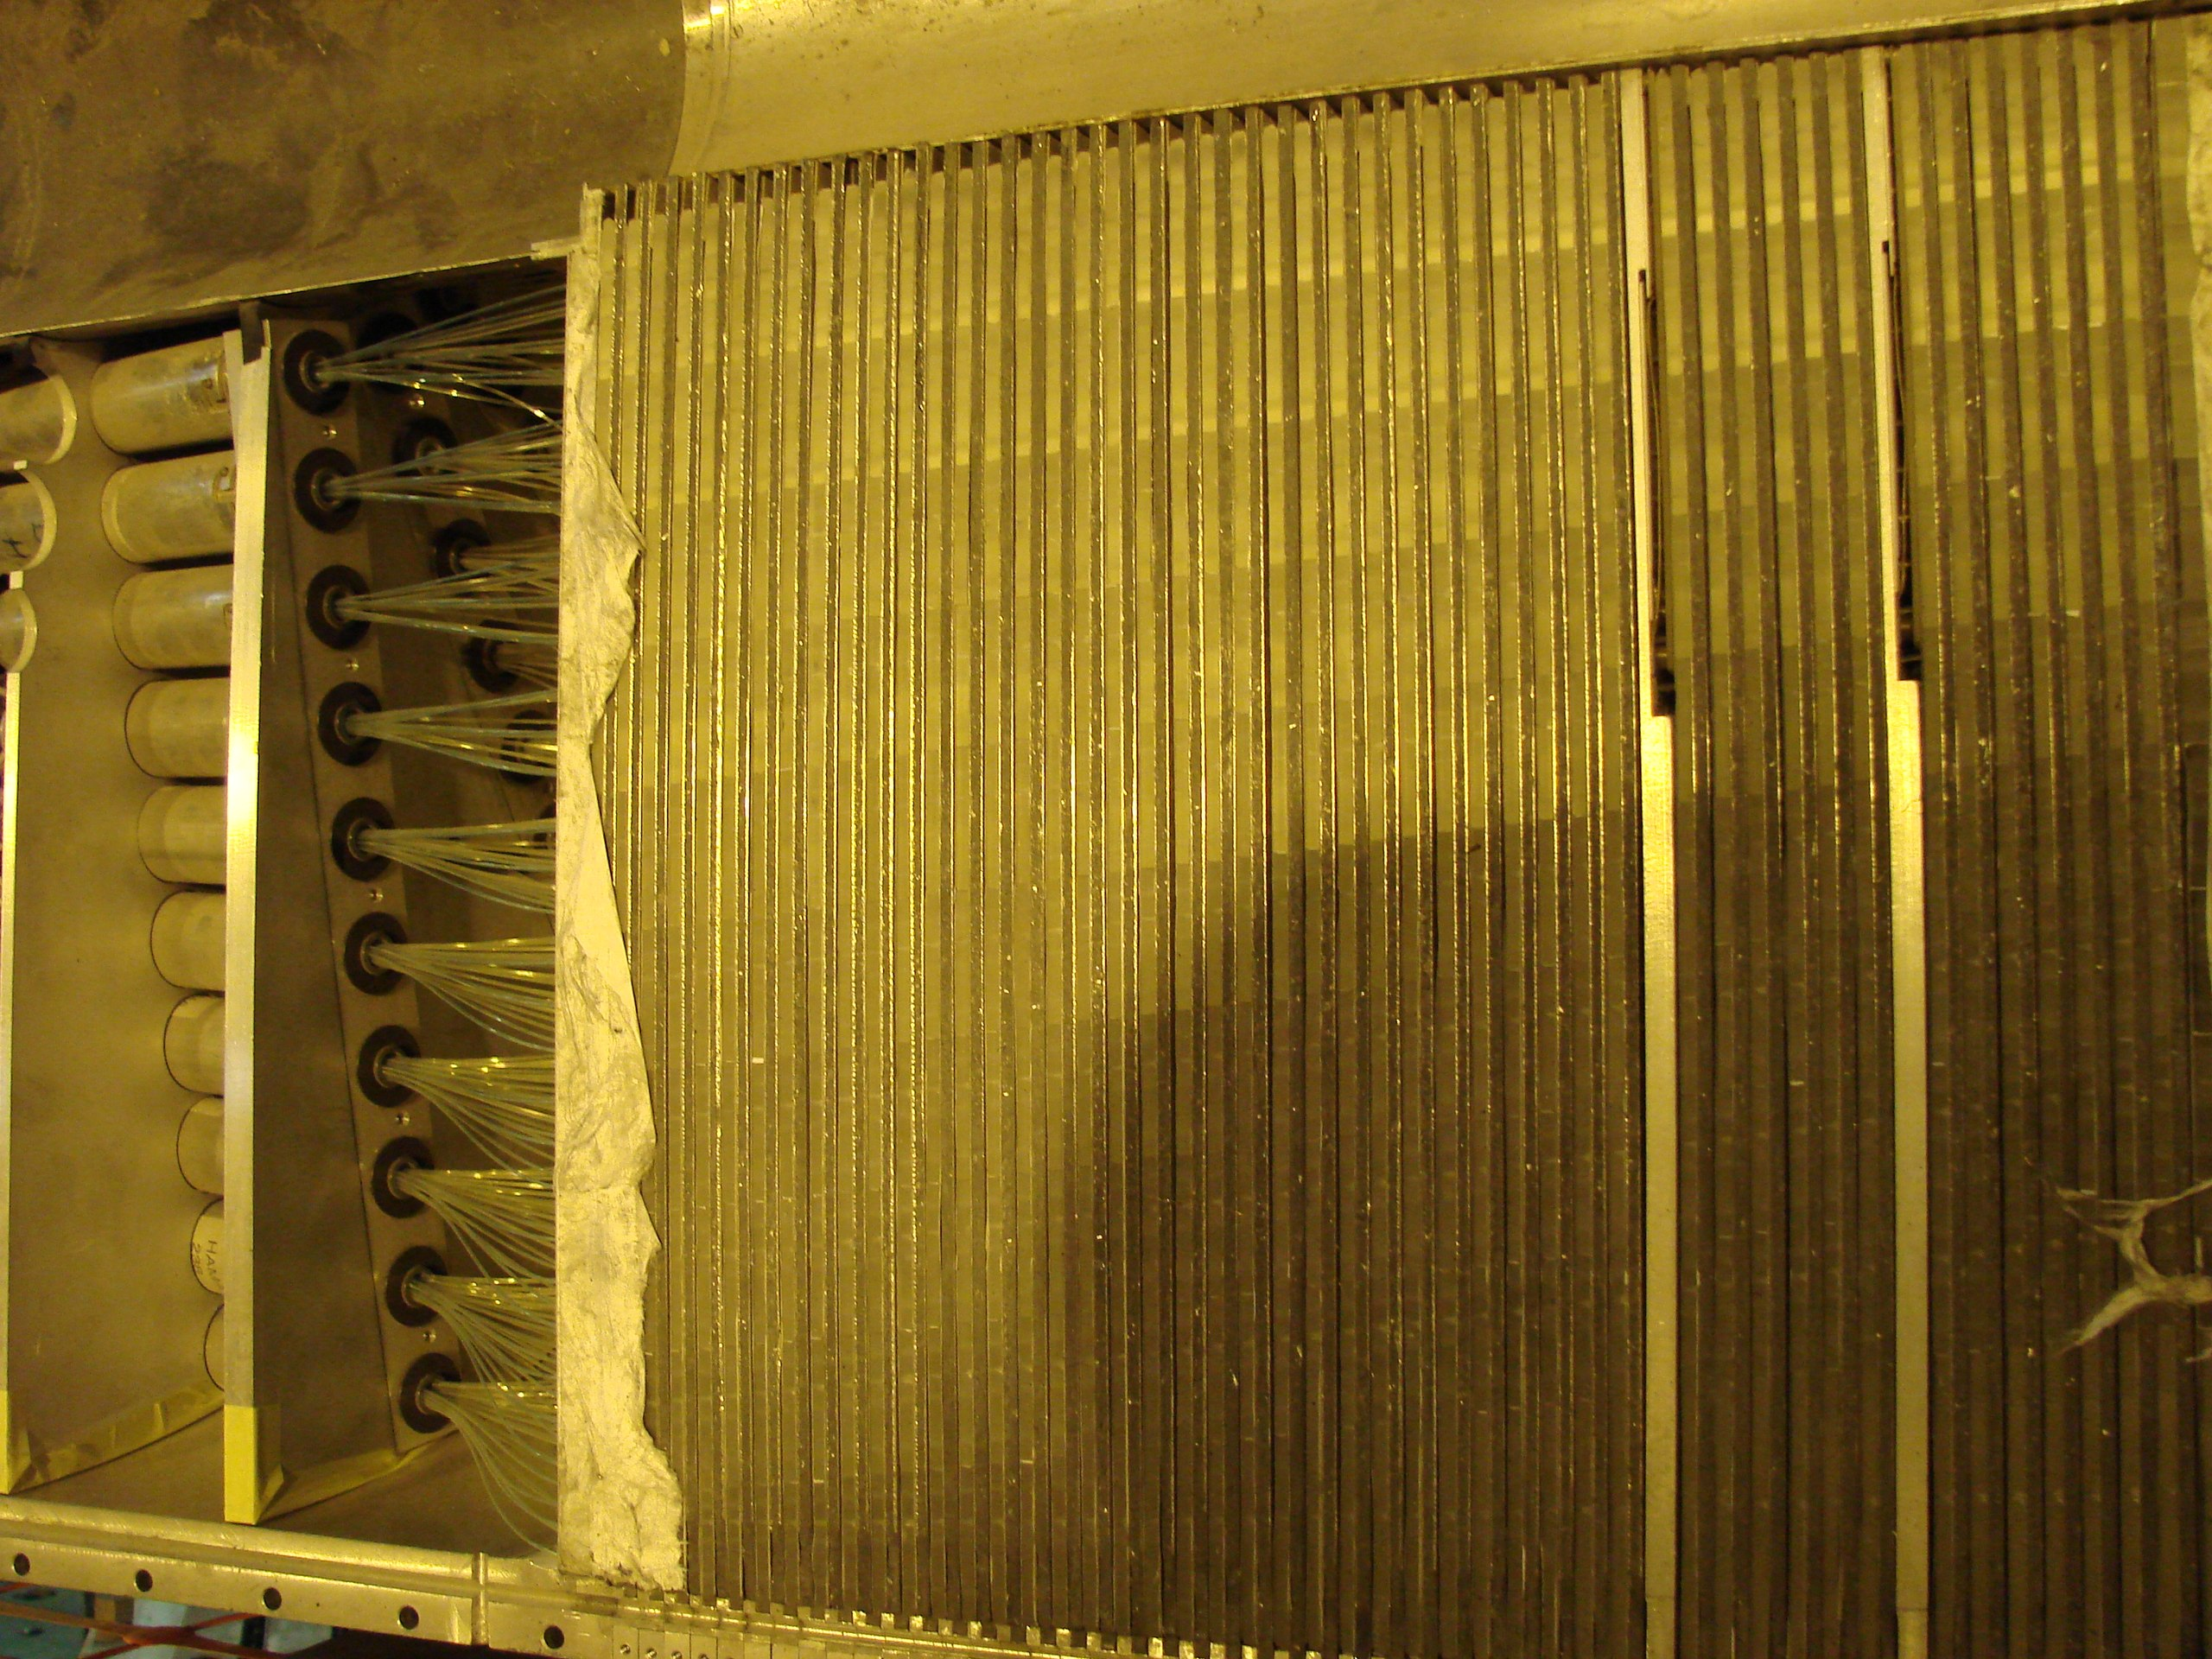
\includegraphics[width=0.7\textwidth]{hcal}
        \end{centering}
    \end{figure}
\end{frame}
\begin{frame}
    \begin{figure}
        \begin{centering}
            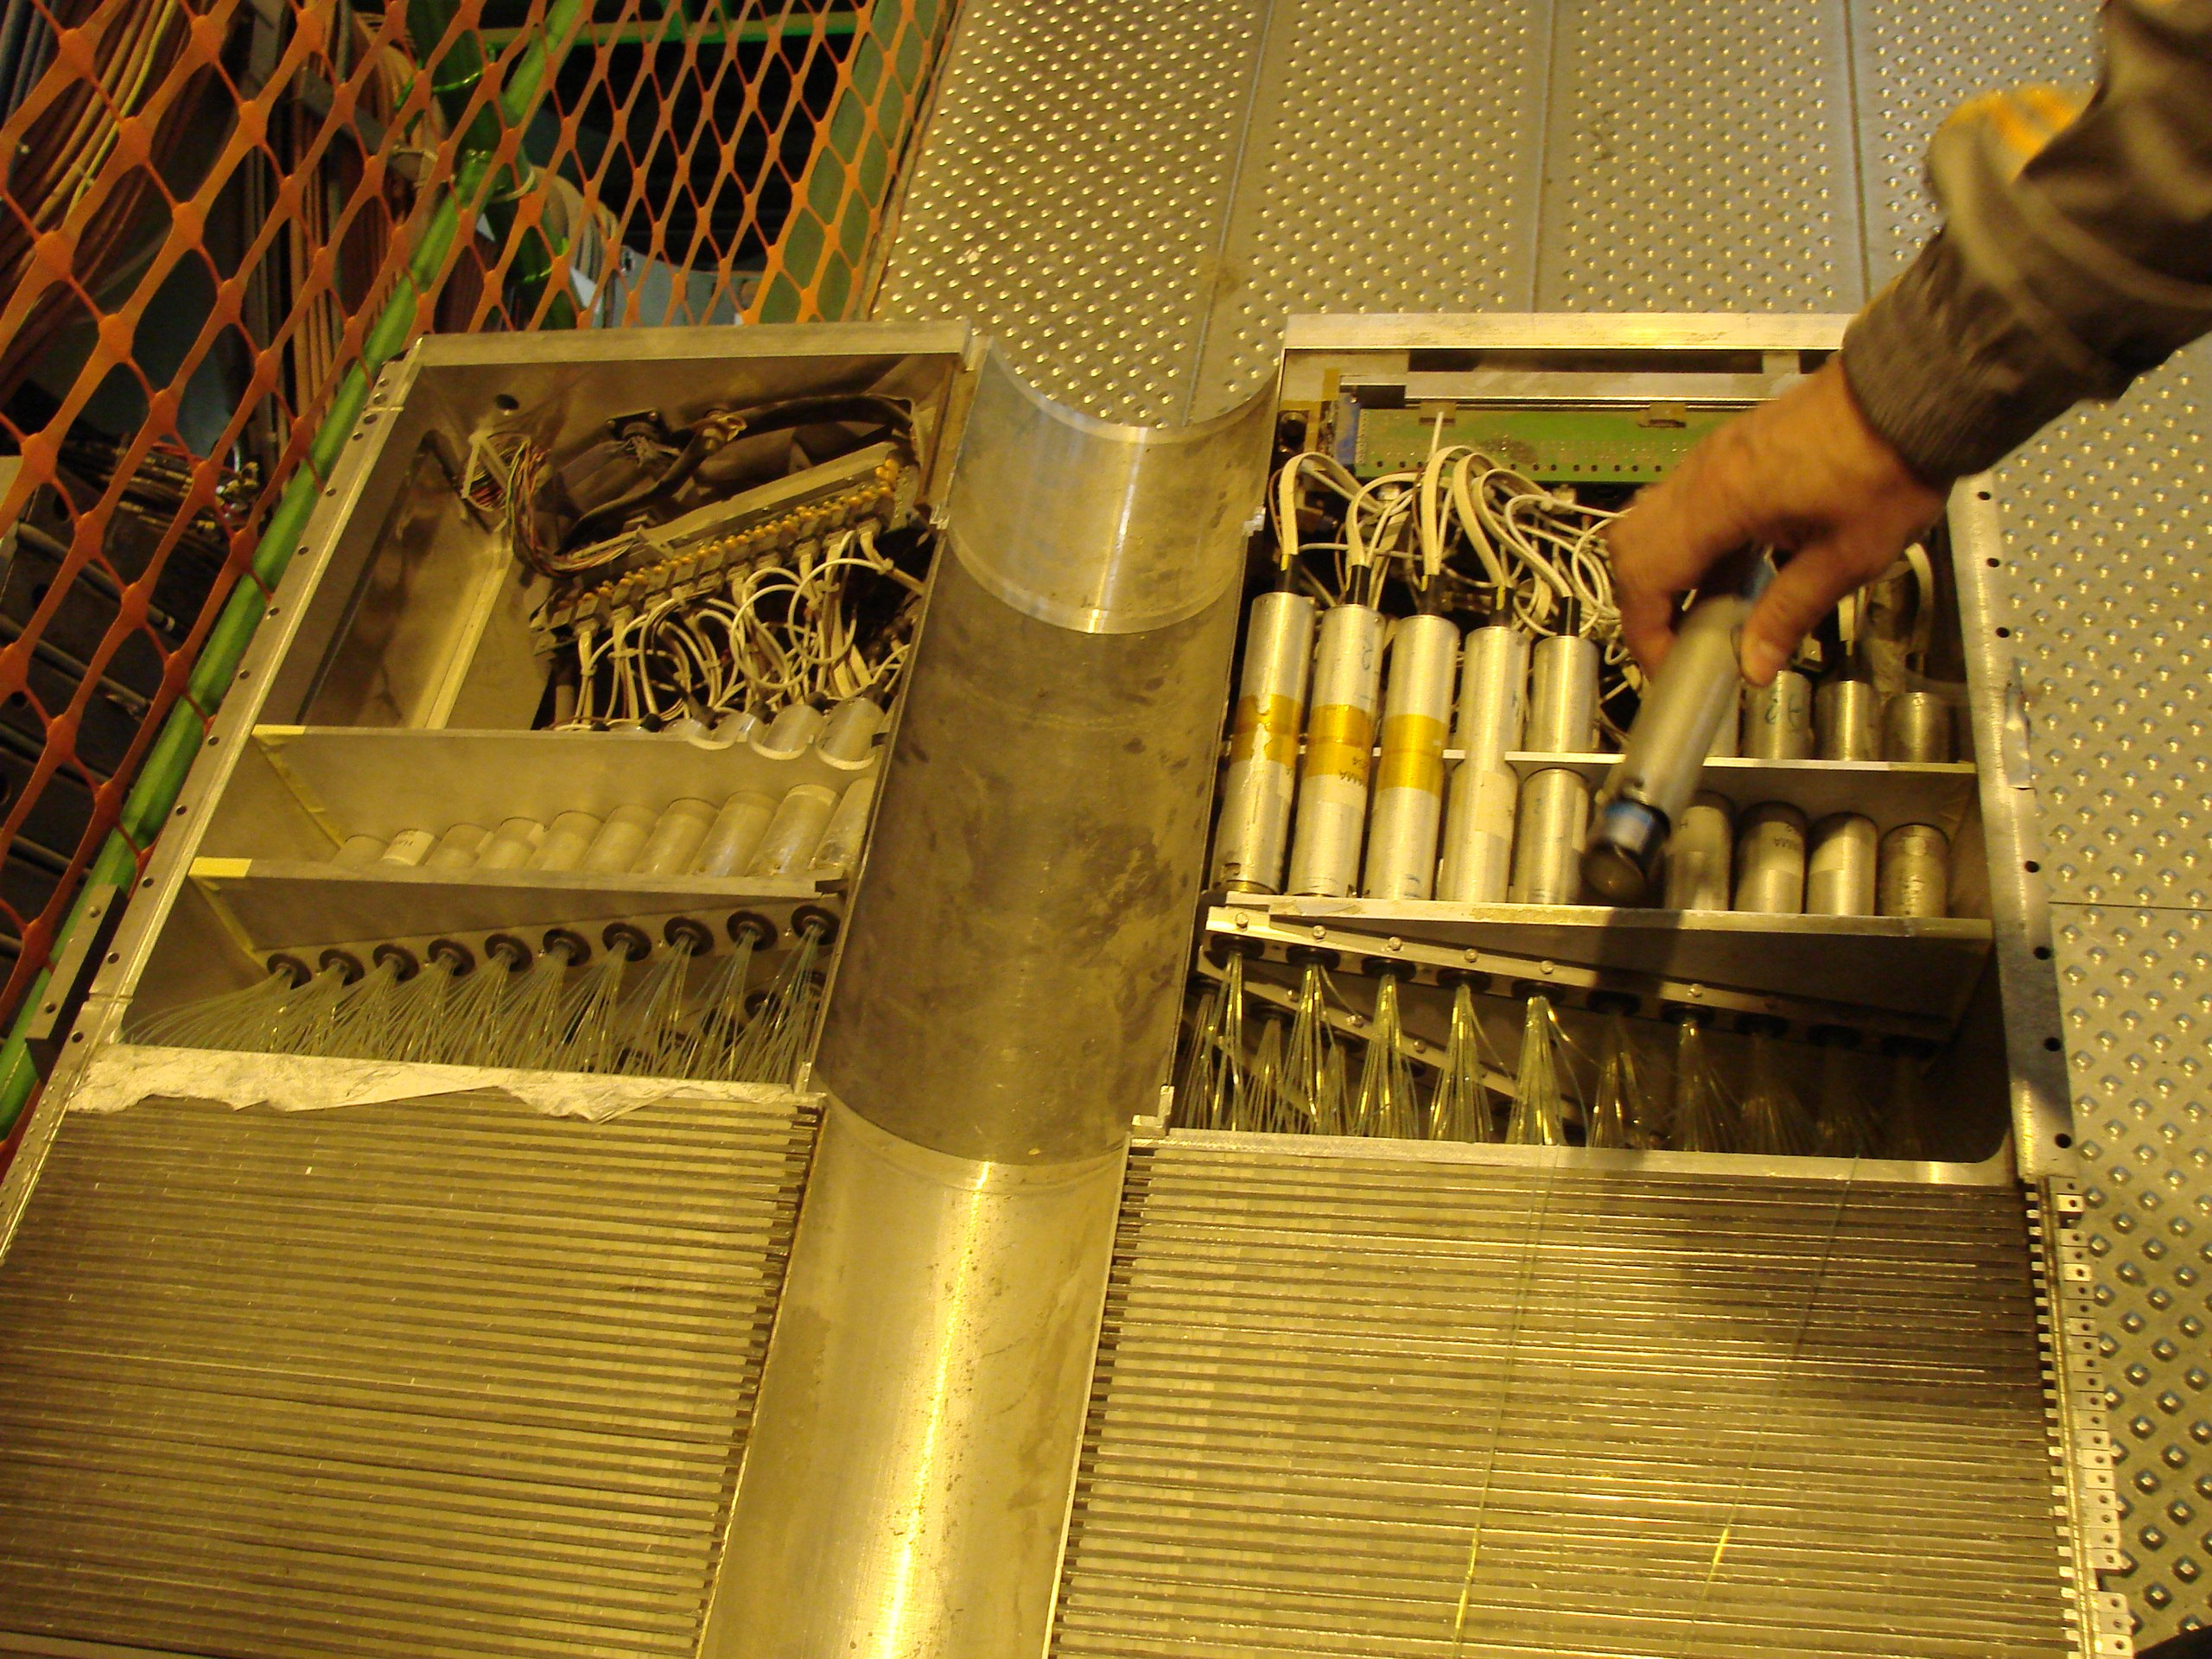
\includegraphics[width=0.7\textwidth]{hcal-pmt}
        \end{centering}
    \end{figure}
\end{frame}
\begin{frame}
    \begin{figure}
        \begin{centering}
            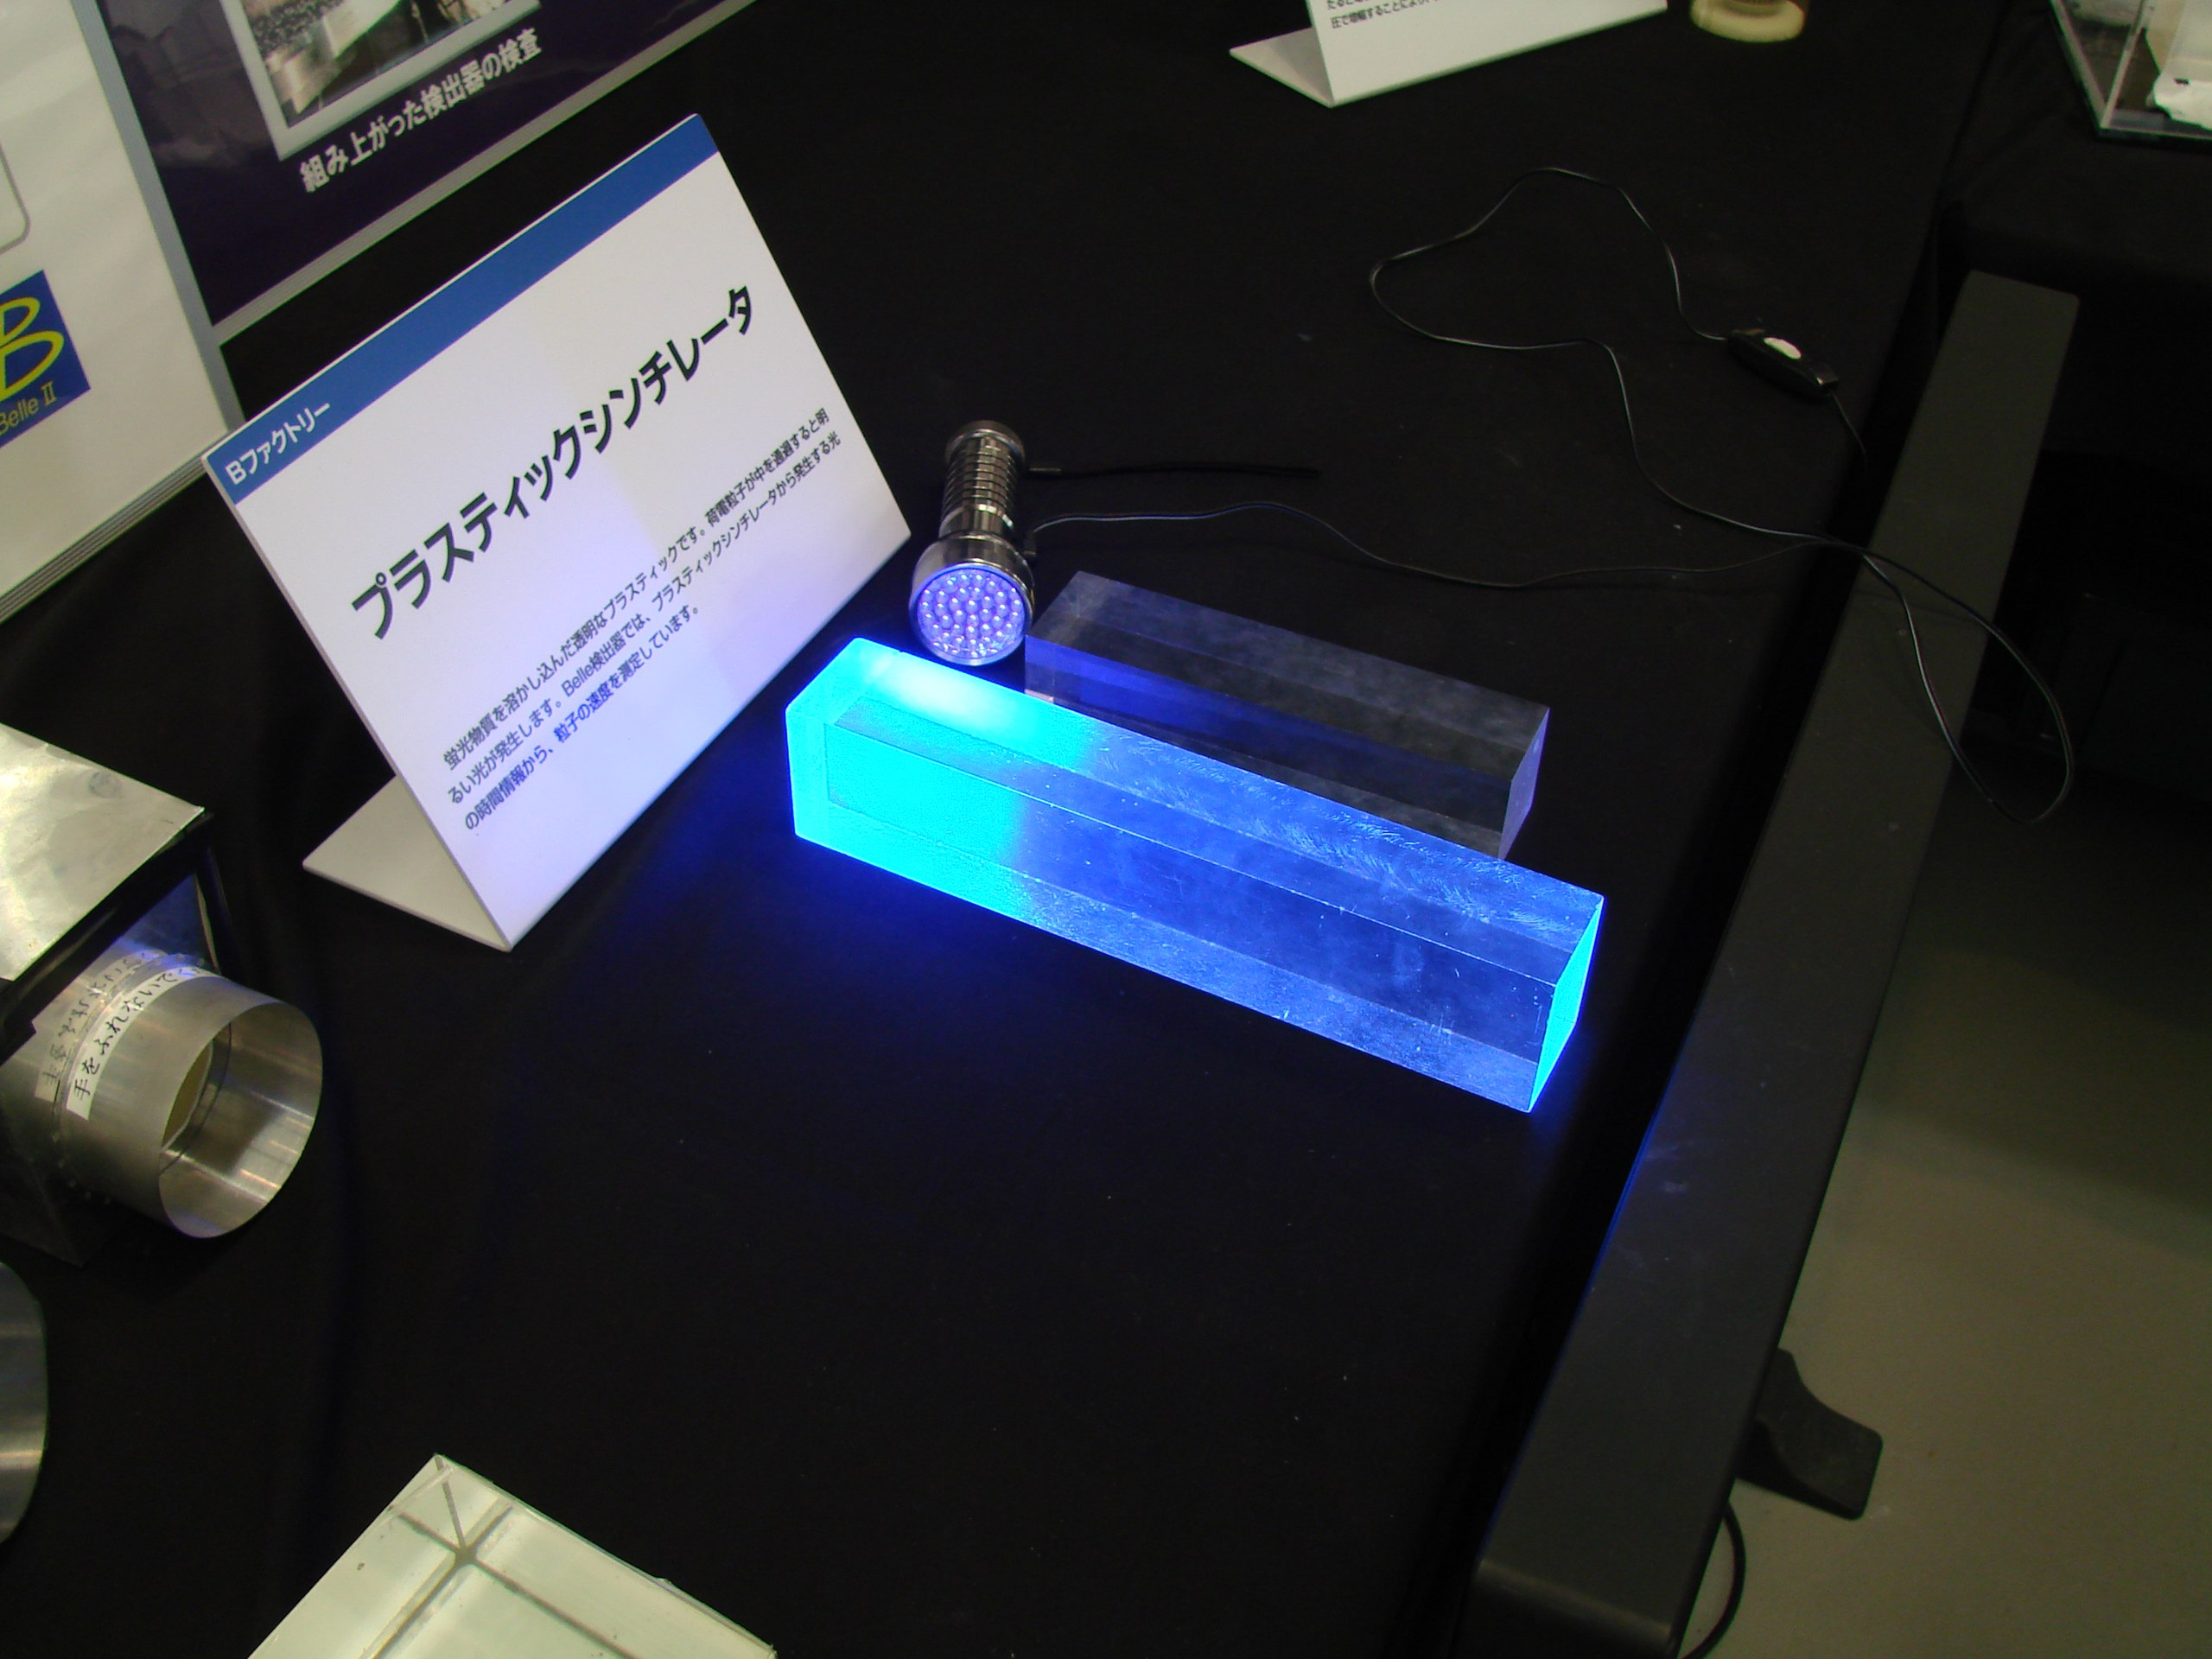
\includegraphics[width=0.7\textwidth]{scintillator}
        \end{centering}
    \end{figure}
\end{frame}

\begin{frame}
    \begin{figure}
    {\LARGE Эволюция ускорителей ЦЕРНа}
    \end{figure}
\end{frame}
\begin{frame}
    \frametitle{Ускорительный комплекс в ЦЕРНе}
    \begin{figure}
        \begin{centering}
            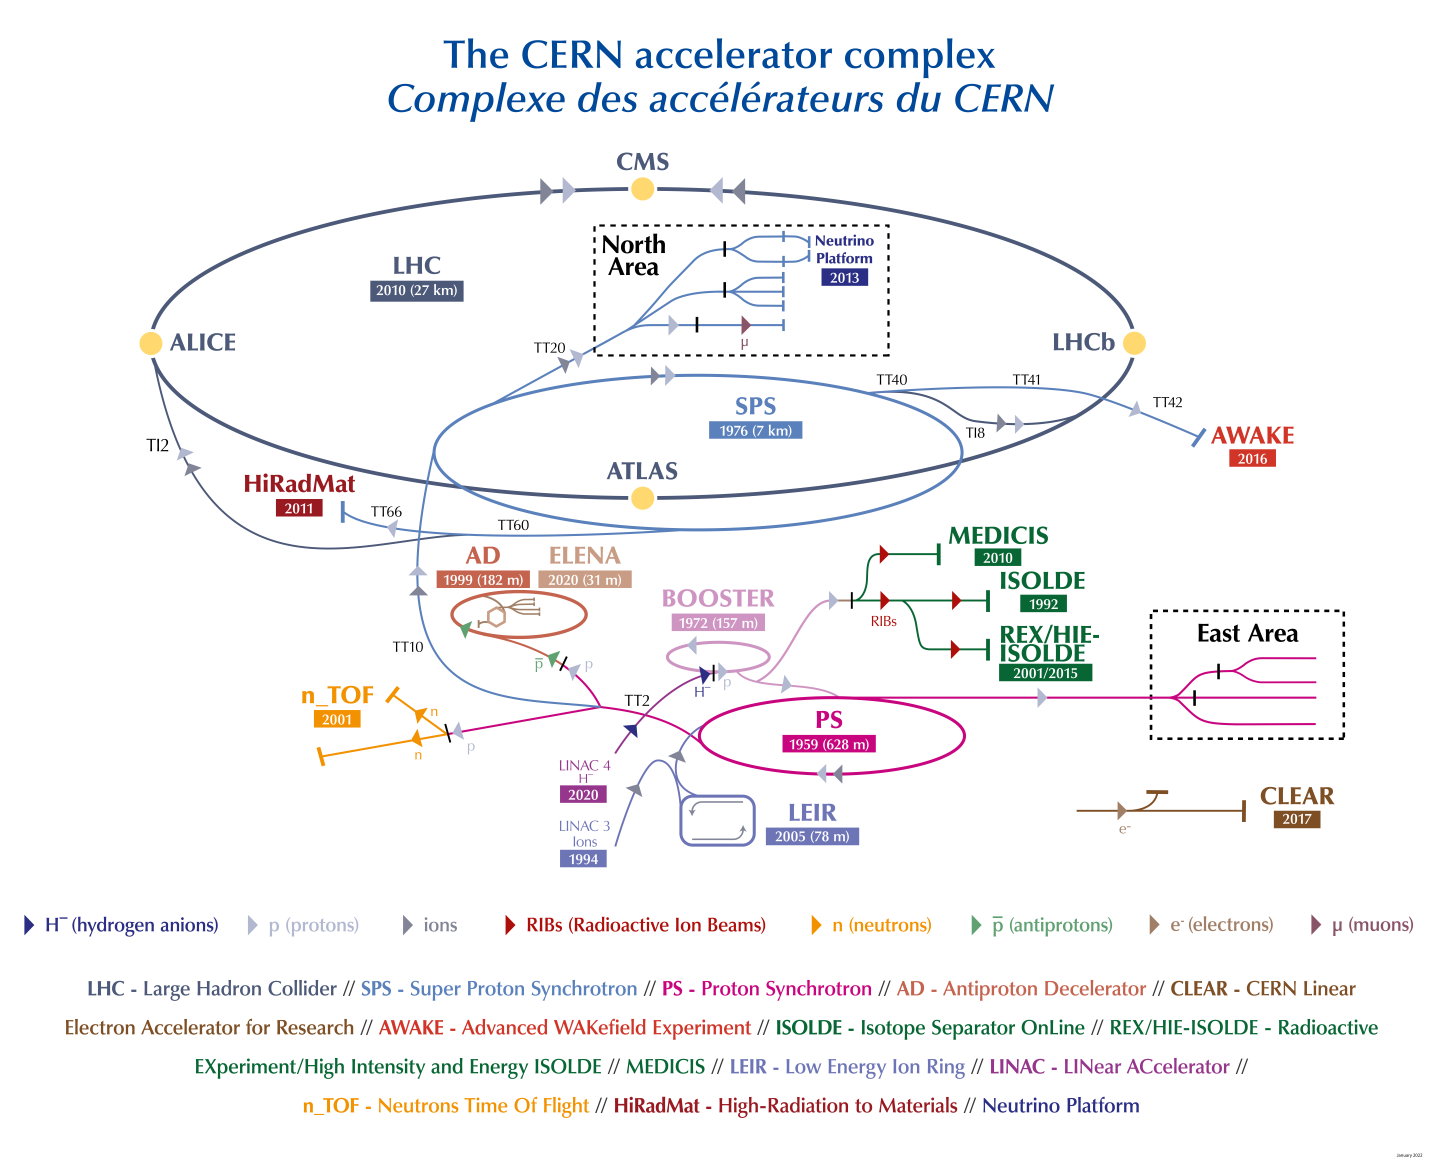
\includegraphics[width=0.7\textwidth]{accelerator-complex}
        \end{centering}
    \end{figure}
\end{frame}
\begin{frame}
    \frametitle{Протонный синхротрон}
    \begin{figure}
        \begin{centering}
            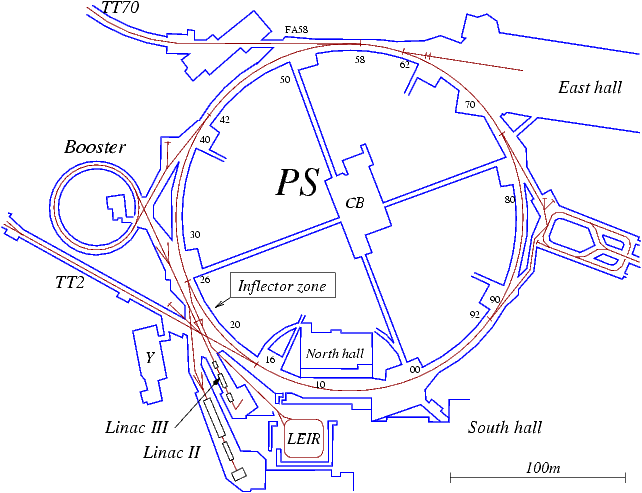
\includegraphics[width=0.7\textwidth]{ps}
        \end{centering}
    \end{figure}
\end{frame}
\begin{frame}
    \frametitle{Супер протон-антипротонный синхротрон}
    \begin{figure}
        \begin{centering}
            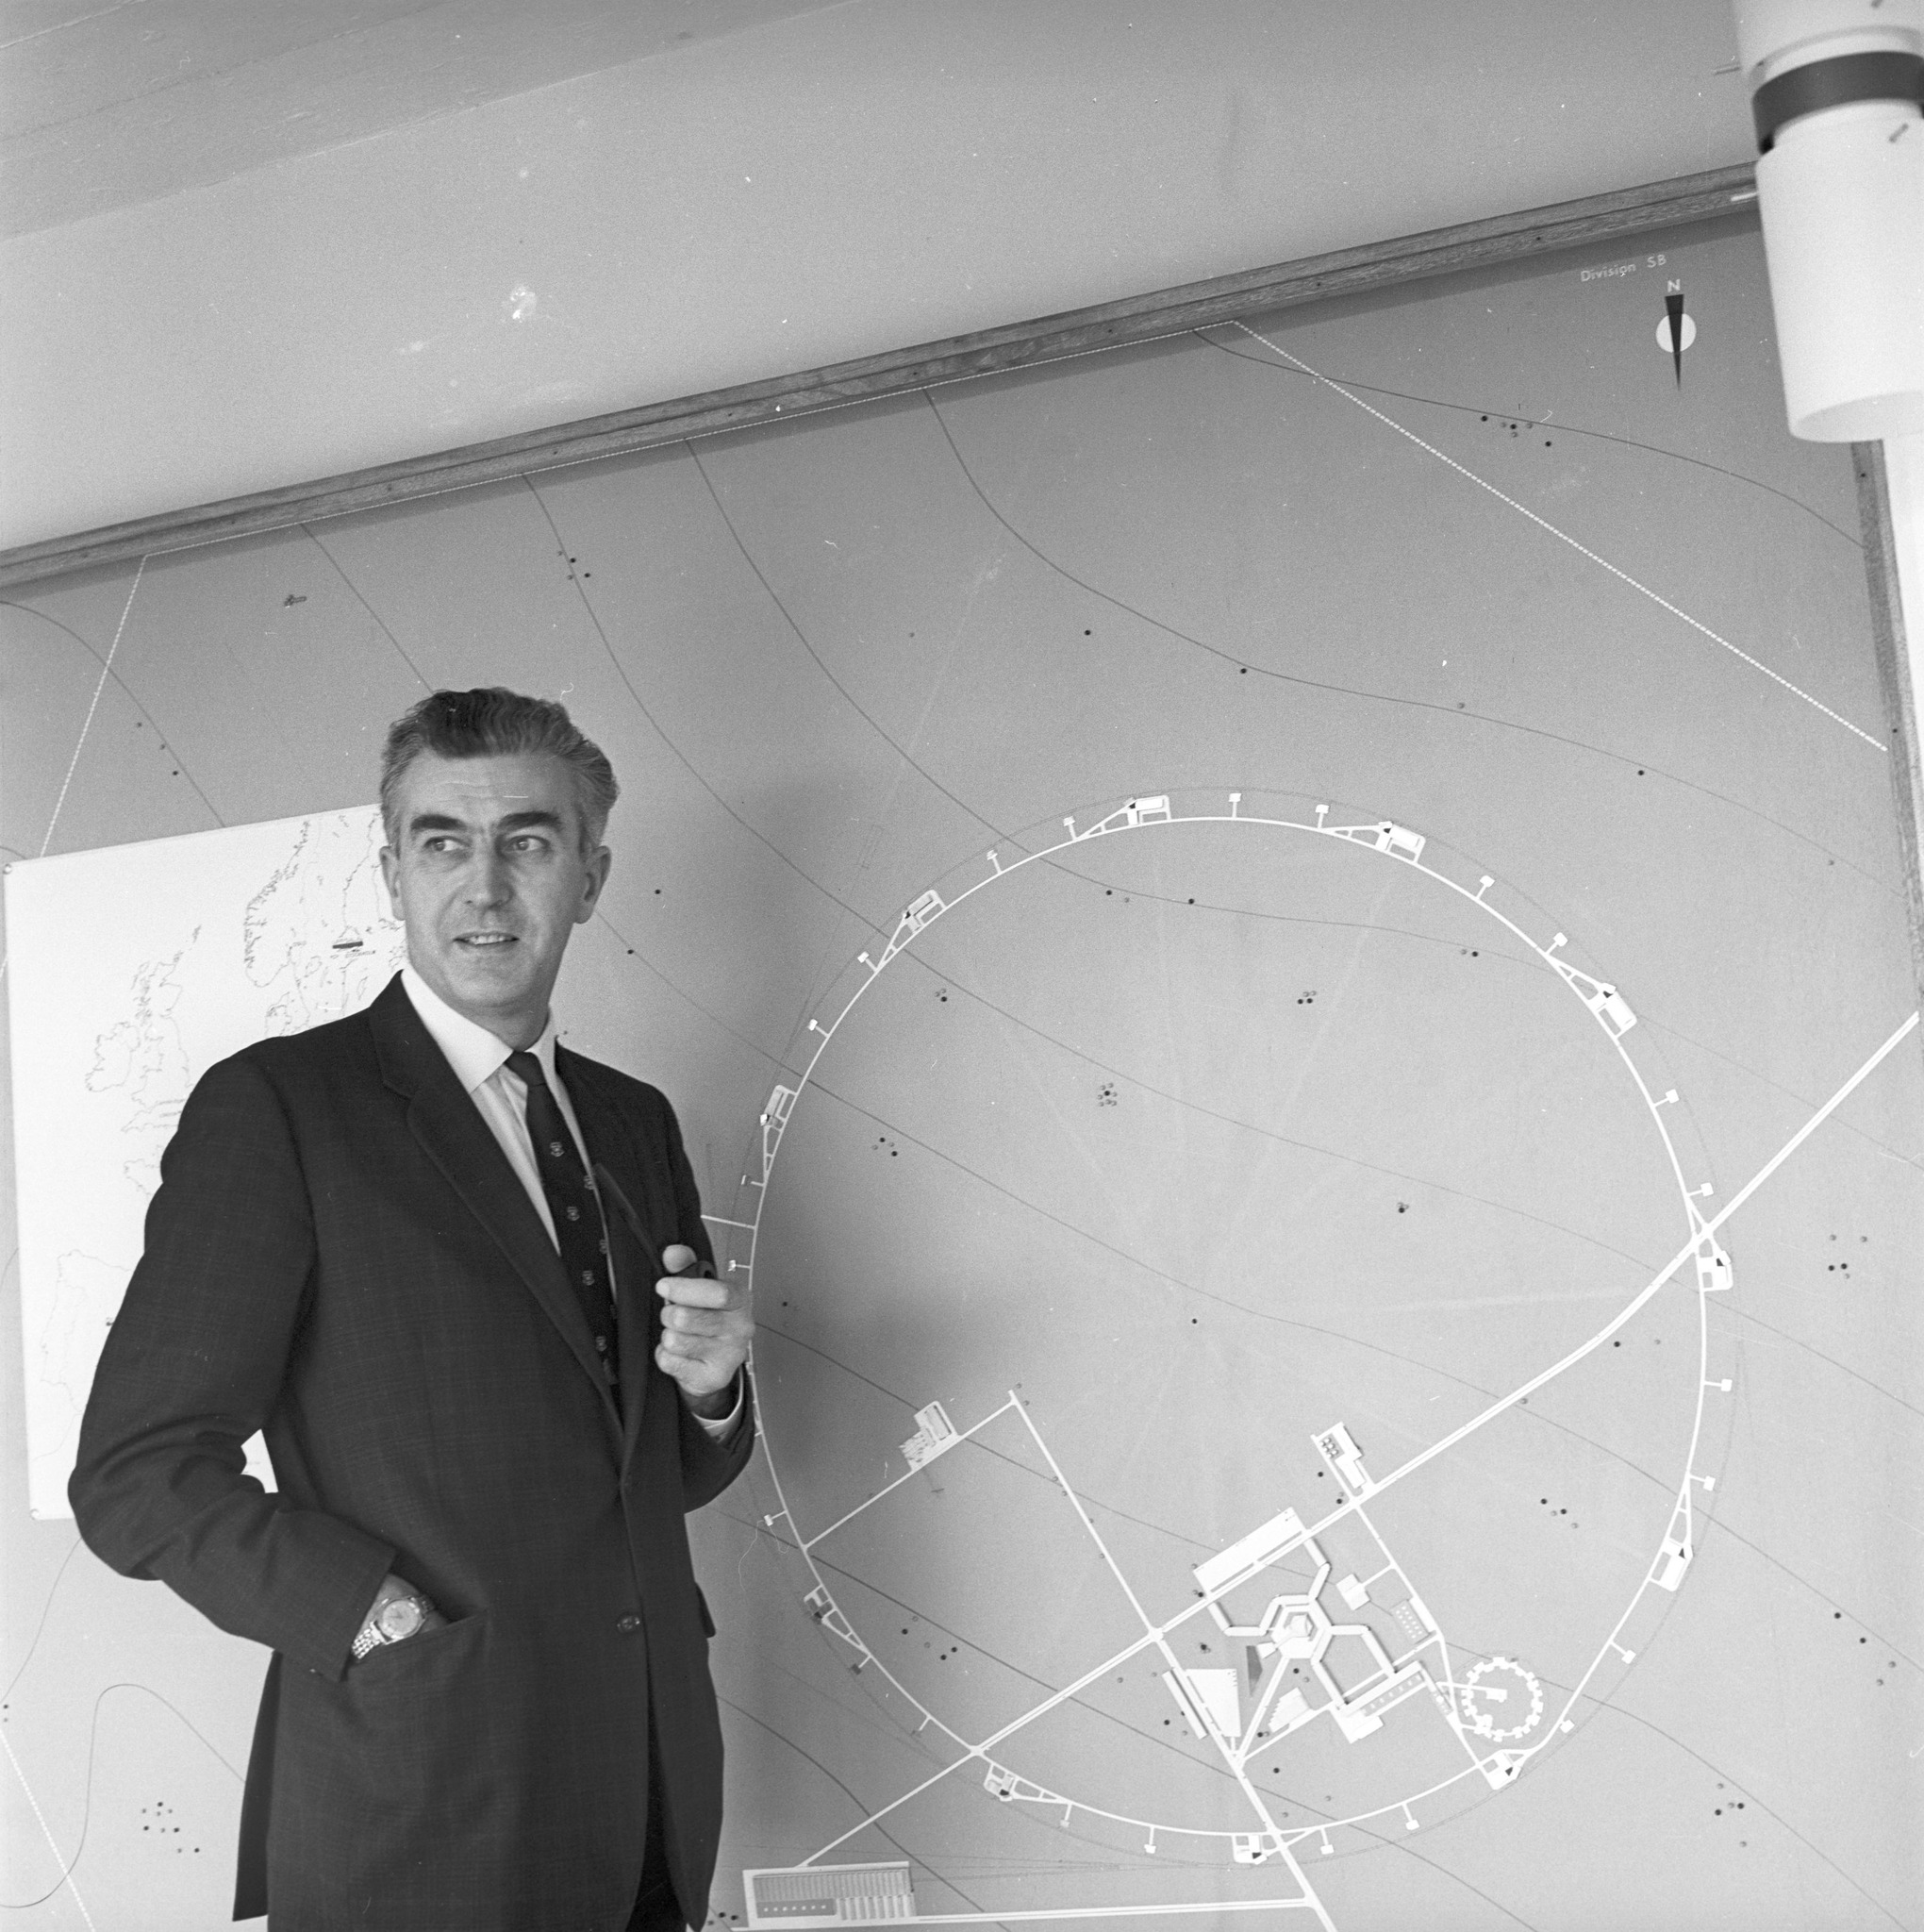
\includegraphics[width=0.5\textwidth]{spps}
        \end{centering}
    \end{figure}
\end{frame}
\begin{frame}
    \frametitle{Большой адронный коллайдер}
    \begin{figure}
        \begin{centering}
            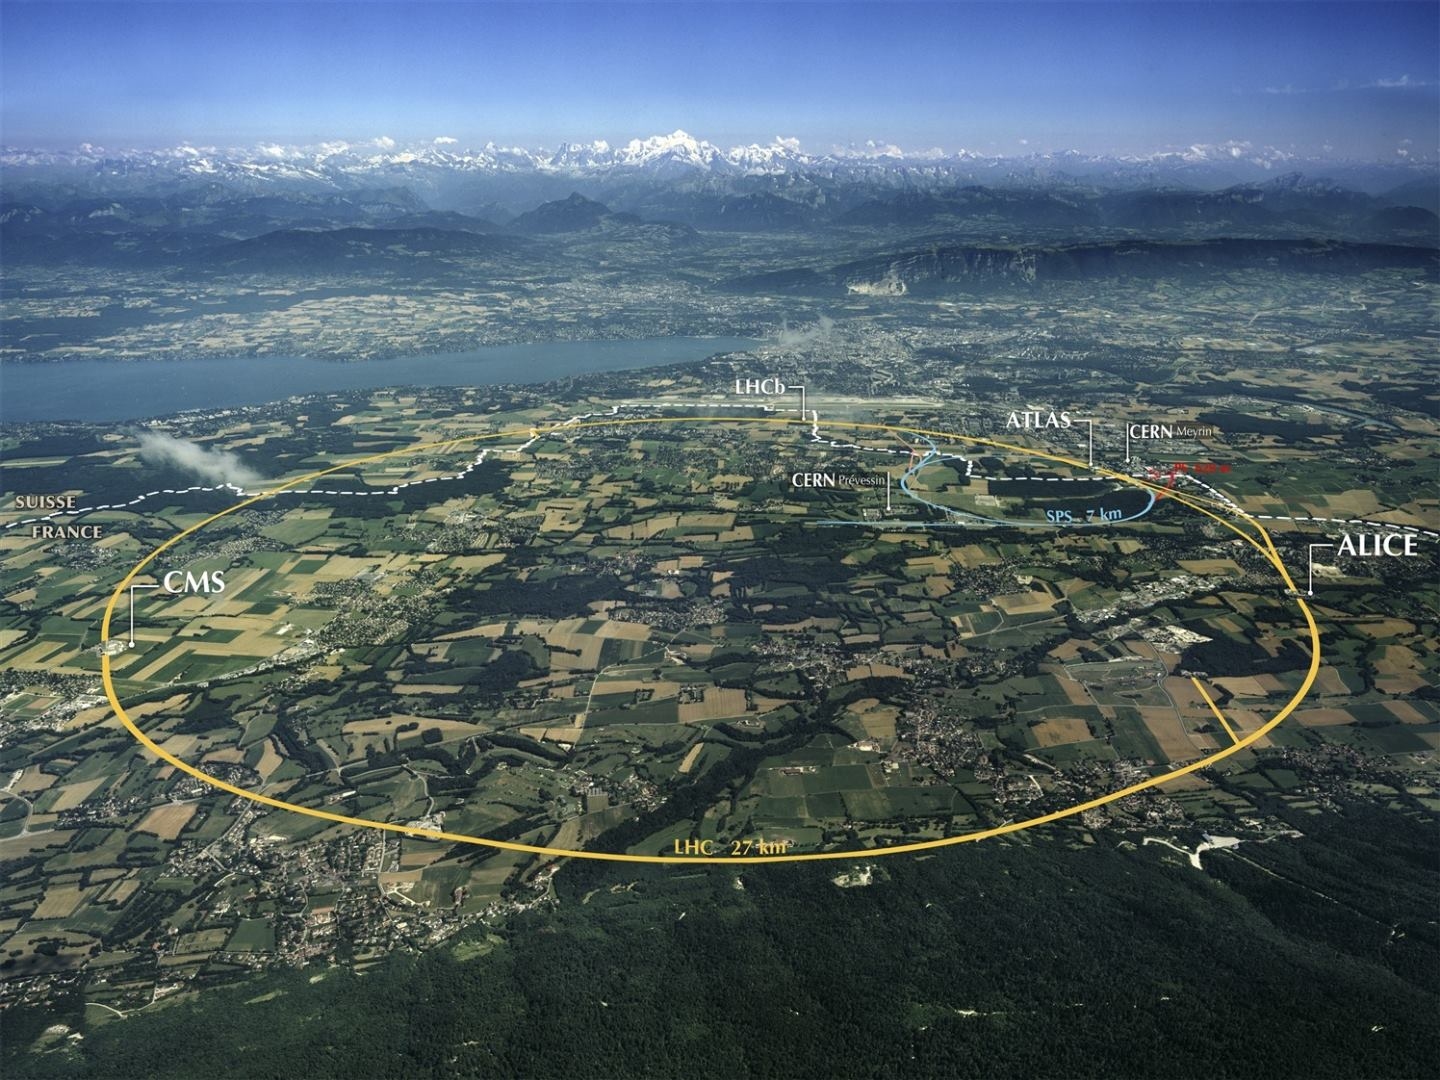
\includegraphics[width=0.7\textwidth]{lhc}
        \end{centering}
    \end{figure}
\end{frame}
\begin{frame}
    \frametitle{FCC: коллайдер XXI века}
    \begin{figure}
        \begin{centering}
            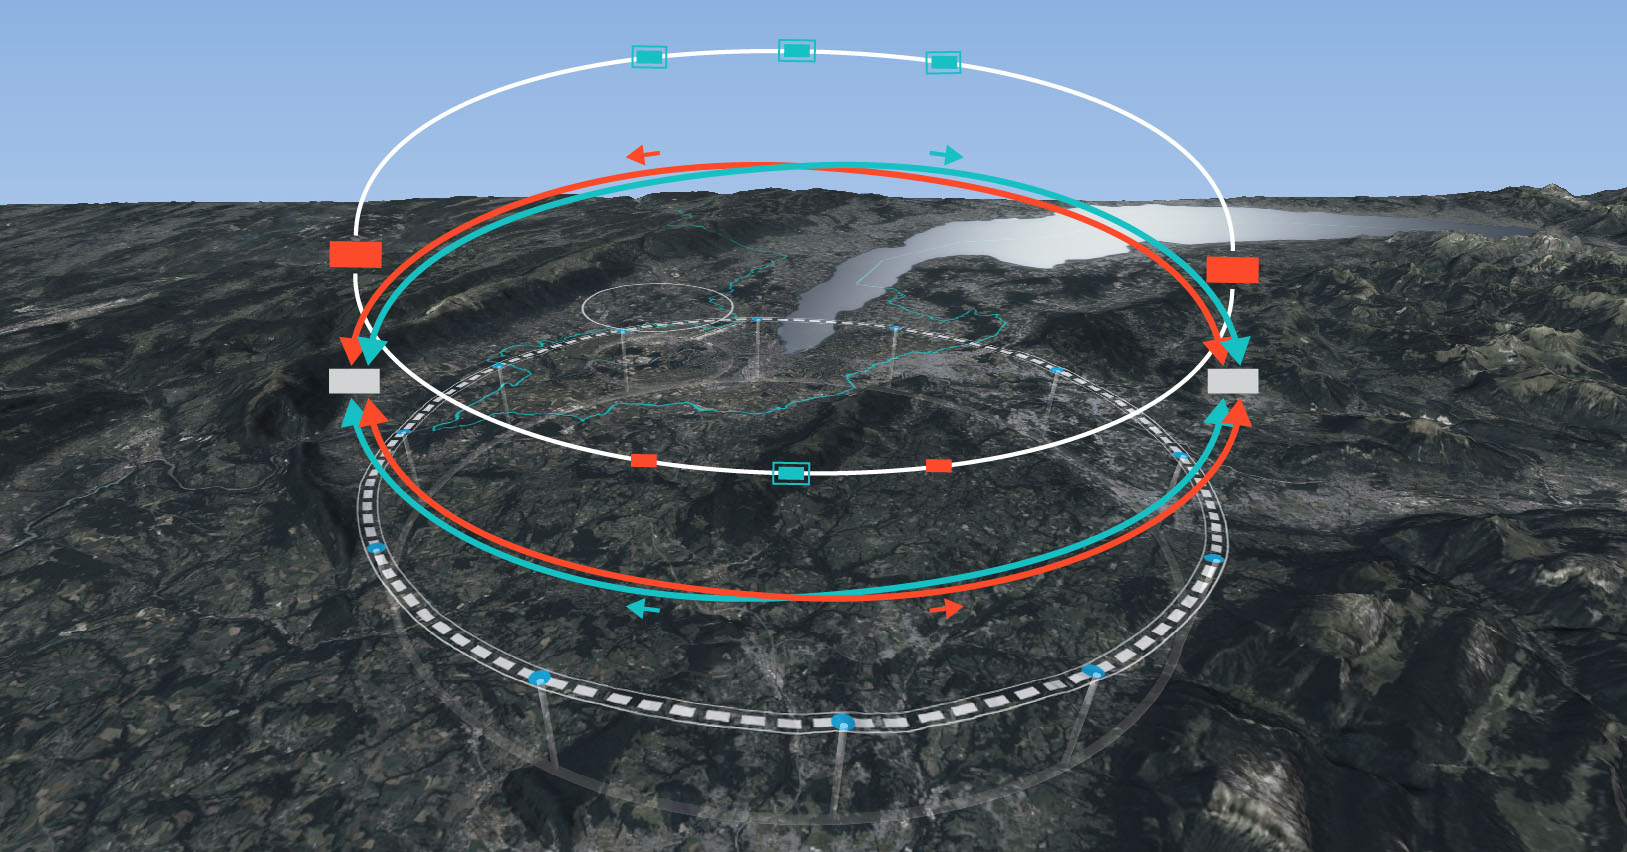
\includegraphics[width=0.7\textwidth]{fcc}
        \end{centering}
    \end{figure}
\end{frame}

\section{Заключение}

\end{document}
